\documentclass[11pt,twoside]{report}
\usepackage{preamble}
\usepackage{standalone}
\graphicspath{
	{../img/ch1/}
	{../img/ch2/}
	{../img/ch3/}
	{../img/ch4/}
	{../img/ch5/}
	{../img/ch6/}
	{../img/ch7/}
	{../img/cha1/}
	{../img/cha2/}
}

\DeclareRobustCommand{\wordcount}
{\InputIfFileExists{thesis.wordcountsum}{}{}
}

\definecolor{bristolred}{RGB}{191,47,56}


\begin{document}

\newgeometry{margin=1in}

%\maketitle
\thispagestyle{empty}
\begin{center}
  \begin{minipage}{0.8\linewidth}
    \centering
    \vspace{3cm}
    {\Large \sc University of Bristol \par}
    \vspace{2cm}
    {\Large \sc Doctoral Thesis \par}
    \vspace{1cm}
    \rule{\textwidth}{0.4pt} \par
    {\LARGE \sc \color{bristolred} 
    Observing, Analysing, Modelling, and even Changing the Behaviour of Zebrafish
    \par}
    \rule{\textwidth}{0.4pt} \par

    \vspace{2cm}
    {\large \it Author:}
    \hfill
    {\large \it Supervisor:} \\
    {\sc \large \href{mailto:yushi.yang@bristol.ac.uk}{Yushi~Yang}}
    \hfill
    {\sc \large Dr.~Thomas~Machon\par}
    \vspace{3.5cm}
   {\large \it A dissertation submitted to the University of Bristol in accordance with the requirements for award of the degree of Doctor of Philosophy in the Faculty of Science, H.\ H.\ Wills Physics Laboratory. \par}
    \vspace{1em}
    {\large March 2022 \par}
  \end{minipage}
  \mbox{}
  \vfill
  \begin{minipage}{0.8\linewidth}
    \raggedleft
    {\large \wordcount}
  \end{minipage}
\end{center}

\pagenumbering{roman}

\cleardoublepage\documentclass[11pt,twoside]{report}
\usepackage{preamble}
\begin{document}

\cleardoublepage
\chapter*{Abstract}
\addcontentsline{toc}{chapter}{Abstract}

\cleardoublepage
\chapter*{}
\vspace*{0.2\textheight}



\noindent\emph{天涯呀~海角 ~~ 觅呀~觅知音} \\[100ex]

\noindent\emph{你的踏板车~要滑向哪里\\你在滑行里~快乐旋转着}


\cleardoublepage
\chapter*{\vspace{-1em} Acknowledgements}
\addcontentsline{toc}{chapter}{Acknowledgements}

Thank you guys!

Francesco; Erika; Paddy; John; Kathleen; Tom;
Levke; Fergus; Max; Laurent; 李静雯 (Jingwen Li);
武晓岳 (Xiaoyue Wu); 陈睿 (Rui Cheng); Katie; Wahab; 陈彦志 (Louis Chen); Jun;
My; Alessandro;
Josh; Peter;
BCFN; Fish Facility; Zebrafish;
王敏 (Min Wang); 杨冬 (Dong Yang);


\cleardoublepage
\chapter*{Author's declaration}
\addcontentsline{toc}{chapter}{Author's declaration}

I declare that the work in this dissertation was carried out in accordance with the requirements of the University's Regulations and Code of Practice for Research Degree Programmes and that it has not been submitted for any other academic award.
Except where indicated by specific reference in the text, the work is the candidate's own work.
Work done in collaboration with, or with the assistance of, others, is indicated as such. Any views expressed in the dissertation are those of the author.

\vspace{1cm}
\vspace{-3pt}

\hspace{2.5cm} {\huge\emph{杨雨诗}} \hspace{5.5cm} 30/01/22 \vspace{-\baselineskip} \vspace{3pt} \\
SIGNED: .............................................................
\qquad
DATE: ..........................

\vspace{1cm}

\section*{Contributions:}

\cite{yang2021pcb}\; \fullcite{yang2021pcb}. \\

\end{document}

\cleardoublepage\tableofcontents

\cleardoublepage\listoffigures
\addcontentsline{toc}{chapter}{List of figures}

\cleardoublepage\listoftables
\addcontentsline{toc}{chapter}{List of tables}

\cleardoublepage\listofalgorithms
\addtocontents{loa}{\def\string\figurename{Algorithm}}

\cleardoublepage
\restoregeometry

%\begin{spacing}{1.25}

\pagenumbering{arabic}

\pagenumbering{arabic}
\setcounter{page}{1}%

\documentclass[11pt,twoside]{report}
\usepackage{preamble}
\graphicspath{{../img/ch1/}}
\setcounter{chapter}{0}


\begin{document}


\chapter{Introduction}

This thesis will discuss the \emph{collective behaviour} of \emph{zebrafish}. And we will start the thesis by describing the individual terms of our topic.

\section{Collective Behaviour}

When objects were densely-packed together, interesting phenomena  appear. And we could call these phenomena as the \emph{collective behaviour} of these things. The collective behaviour is interesting because ``more is different'' \cite{anderson1972}. In other words, the behaviour of a large group can not be predicted, even if we know precisely the fundamental laws for the individuals.

An example to illustrate the complexity of collective behaviour, is a collection of randomly packed balls. When we randomly pack a lot of plastic balls together, they packed together like those in Fig.~\ref{fig:random-pack}. These plastic balls, often modelled as \emph{hard spheres}, have a simple property that two spheres can not be too close so that they overlap.
Surprisingly, the accurate prediction of the density (expressed for example as the volume fraction) of the randomly packed hard spheres is still unachieved\marginfootnote{
The latest progress about this problem was made by \citeauthor{zaccone2022} \cite{zaccone2022}. But the proposed solution received many criticisms \cite{blumenfeld2022, charbonneau2022, chen2022}.
} \cite{kamien2007, zaccone2022}.
In addition, the well packed hard spheres form a collection of clusters with different geometrical features. In Fig.~\ref{fig:random-pack} two different clusters were highlighted. The prediction of the geometrical features is still a challenging problem \cite{malins2013, robinson2019}.

The collective behaviour of objects with varying lenght-scales were studied, from atoms, to colloids, animals, as well as human beings \cite{walker1990, lekkerkerker1992, becco2006, henderson1971, silverberg2013}. The interesting feature of their collective behaviour is the transformation from one phase to another under different conditions \cite{sethna2006}. For instance, the water could change between the fluid phase and crystal phase under different temperatures. These behaviours are often noted as \emph{phase behaviour}, and summarised by \emph{phase diagrams}. The phase diagrams of systems in equilibrium have been systematically studied. However, the equivalent in non-equilibrium systems were less studied, and they will be introduced in chapter~\ref{chapter:collective_behaviour}.

\marginpar{
\centering
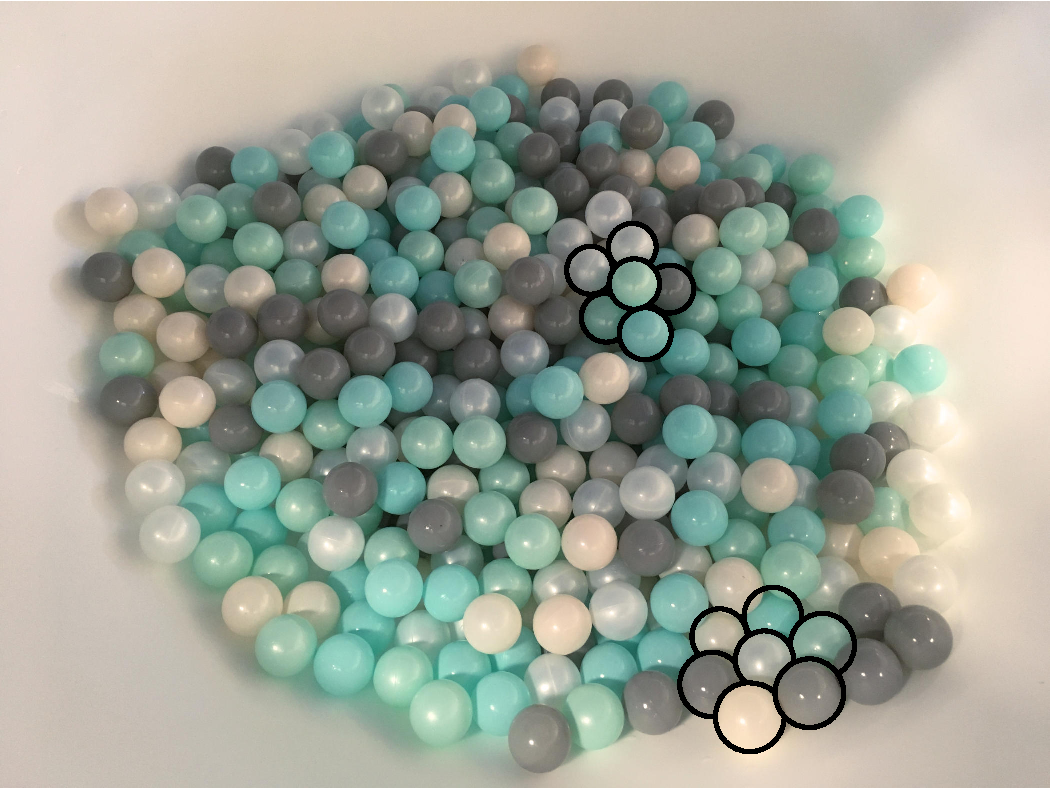
\includegraphics[width=\marginparwidth]{random-pack}
\captionof{figure}[Randomly packed plastic balls.]{
  A photo of randomly packed plastic balls. The photo was taken by the author.
}
\label{fig:random-pack}
}


\section{Zebrafish}

Zebrafish (\emph{Danio rerio}) is a small fish living mainly in  India and Bangladesh, as well as in areas of Pakistan, Nepal, and Myanmar \cite{neff2020}. These fish are social animals that form small groups in the size of tens in still water \cite{suriyampola2016}. In rivers with faster flow, the group size could be thousands \cite{shelton2020}. The photo of a typical adult zebrafish is shown in Fig.~\ref{fig:fish}, with the characteristic stripes of this species. Placing a group of these fish together, they will interact with each other, and often form a coherent group. These behaviours are what we will be studying through out this thesis.


\marginpar{
\centering
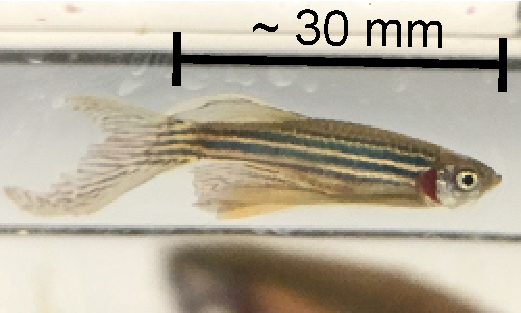
\includegraphics[width=\marginparwidth]{zebrafish}
\captionof{figure}[The photo of a zebrafish]{
	The photo of an adult zebrafish. The photo was taken by the author.
}
\label{fig:fish}
}

Zebrafish receive attention from the scientific community, because they present a good animal model for different human diseases. Being a vertebrate, the genome of zebrafish is similar to that of human beings \cite{howe2013}. In addition, the embryo of zebrafish, as well as the zebrafish larva are transparent \cite{kimmel1995}, making microscopic observation of cellular behaviour very easy. With the help of zebrafish, we could study common diseases such as the osteoarthritis \cite{lawrence2018, kague2021}, autism \cite{kim2017}, and cancer \cite{lopez-cuevas2021}. The appeal of zebrafish as an animal model makes them being widely used in different institutions\cite{spence2007}. Practically, the zebrafish in the laboratory were kept in a standard condition for many generations \cite{westerfield2000}. These fish are less likely to suffer from common diseases and parasites, comparing with wild captivated fish \cite{spence2007}. These fish are good for behavioural experiment as their living condition are controlled, which makes repeating experiments easy. In this thesis, all the zebrafish were bred at the fish facility of the University of Bristol.

There are multiple reasons to study the collective behaviour of the zebrafish. The first reason is technical. The fish naturally swim in the river, where they can change their depth every now and then. Observing the fish swimming in a three dimensional (3D) space requires advanced tracking system. The design and construction of such 3D underwater tracking system is a technical challenge. And it is meaningful to solve this challenge. In addition, understanding the behaviour of zebrafish could help us differentiate the states of the fish. And we will have predictive power about the fish behaviour, if we could construct a phase diagram of the fish. Finally, we may study the behavioural difference of the mutant zebrafish, to understand the consequences of genetic modifications.


\section{Thesis Structure}


In the next chapter the ideas of active matter and the collective behaviour of animals will be discussed.
We will draw the similarity between a group of animal and a group of synthetic particles under constant energy input. 
Typically, we will stress the complex patterns formed by the animals. The statistical analysis of these patterns will be discussed, as well as some mathematical models that explained the behaviour.

The following two chapters, chapter~\ref{chapter:fish_2d} and \ref{chapter:fish_3d}, will address the technical challenges for the construction of a 3D fish tracking system. Firstly, the method to record the 2D movements of the zebrafish will be discussed in chapter \ref{chapter:fish_2d}. The important element in chapter~\ref{chapter:fish_2d} is the image processing methods, which enables us to extract features from the images. The density distribution of the fish in a quasi-2D environment will also be discussed in chapter~\ref{chapter:fish_2d}. 
Then we will move to chapter~\ref{chapter:fish_3d}, which discussed the construction of a 3D tracking system. 
This chapter will mainly feature different algorithms to calculate the 3D locations of the fish, following the ideas  of multiple view geometry. The experimental results of 3D tracking will also be discussed in chapter \ref{chapter:fish_3d}.


The tracking system will first produce the coordinates of the fish, which provides the information about the structure of the fish group. To study the dynamics of the fish, the coordinates needs to be linked into trajectories. The linking method will be introduced in chapter~\ref{chapter:fish_analysis}. From the trajectories, we can study the structure and the dynamics of the fish with analytical methods developed in the active-matter community. The analysis includes the calculation of different quantities that capture the essence of the fish behaviour, as well as the calculation of the \emph{correlations} of different quantities. These analytical methods will be introduced, and applied to the experimental data. As a result, an important behavioural feature of the fish will be revealed in the end of chapter~\ref{chapter:fish_analysis}.


To further understand the fish behaviour, typically the analytical results, we will try to construct models that reproduced the behaviour. We will model the fish as identical agents following certain rules. We will make the model behave like the real fish, by adjusting the model parameters to match the analytical results. The fitted model will then serve as explanations for the observed results. Specifically, we will try to understand the density distribution of the fish, as well as the dynamics of the fish with different models.


Afterwards, we will move to a more biological topic and discuss the behaviour of zebrafish after genetic modification. In chapter \ref{chapter:fish_mutation}, the collective behaviour of the mutant fish will be reported and compared against the normal, wildtype zebrafish.
%The insight into the mutation fish is only available through the behavioural experiments, as t
The mutant fish have a longer orientational relaxation time compared with the wildtype fish.
The change in the single-fish property will affect the collective behaviour of the fish, making a group of mutant fish exhibiting more ordered movement, which can be explained by an active matter model from chapter~\ref{chapter:fish_model}.


Finally, we close the thesis with a conclusion that summarised all experimental observations, analytical results, as well as the models, and discussed possible future tasks to further improve our understand of the zebrafish behaviour.

\end{document}
\documentclass[11pt,twoside]{report}
\usepackage{preamble}
\graphicspath{{../img/ch2/}}
\setcounter{chapter}{1}


\begin{document}


\chapter{The Collective Behaviour of Animals as Active Matter}
\label{chapter:collective_behaviour}

\epigraph{We declare that the splendour of the world has been enriched by a new beauty: the beauty of speed.}{F. T. Marinetti\\ \emph{Manifesto of Futurism}}

\section{Active Matter}
\label{section:active-matter}

This chapter would discuss the collective behaviour of \emph{active matter}, focusing on the behaviour of \emph{animals}.
The term \emph{active matter} refers to a class of non-equilibrium systems, whose constituting individuals constantly consume energy to generate systematic motion \cite{ramaswamy2017}. These individuals are called \emph{active particles}, and they often propel themselves along the direction of their \emph{orientations} \cite{romanczuk2012}.


\subsection{What is the activity?}


\marginpar{
\centering
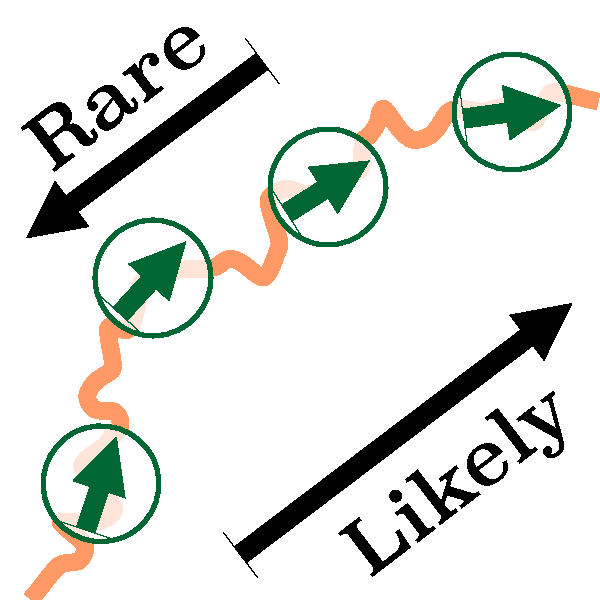
\includegraphics[width=\marginparwidth]{active-trs}
\captionof{figure}[The trajectory of a single active particle]{
	The trajectory of a single active particle, which breaks the time-reversal symmetry. The arrow in the circle represents the orientation of the particle, the direction of the self-propelling force.
}
\label{fig:active-trs}
}


Active particles are different from their passive counterpart in equilibrium systems, because of their ``activity''. The activity could be defined, roughly as the ratio between the deterministic, self-propelling movement, and the stochastic movement from thermal fluctuation.
The self-propelling movement breaks the time-reversal symmetry (\gls{TRS}), making the movement of active particles special \cite{obyrne2022}.
One example of how one active particle breaks the TRS is shown in Fig.~\ref{fig:active-trs}. The self-propelling particle, represented by the circles in Fig.~\ref{fig:active-trs} would have an orientation vector, illustrated by the arrow Fig.~\ref{fig:active-trs}.
This orientational vector is an internal degree of freedom of the particle, like a spin carried by the particle.
The particles would generate motion in the direction of their orientation vector, being self-propelling. An active particle is more likely to form a trajectory, where the particle is always moving along its orientation, rather than moving against its orientation.
For instance, the orange line in Fig.~\ref{fig:active-trs} is more likely to be the trajectory of an active particle that is moving upwards, because the orientations of the particle are pointing at similar directions. It is very unlikely to observe a particle to form such trajectory by traveling from upper right to lower left, if the particle is active\marginfootnote{
It is still possible for the rare situation to happen, but the motion had to be driven by randomness. For instance, an active colloids might move against its propelling force, because of the random kicks from solvent molecules. 
}.
In the absence of activity, where the particle is in equilibrium, the two different options in Fig.~\ref{fig:active-trs} would have the same probability.

The Péclet number (\gls{Pe}) is often used to quantify the activity of the particles \cite{bechinger2016}. It is defined as the ratio between the driven, deterministic motion, and the random, diffusive motion.
It is easy to grasp the effect of activity visually, by inspecting the movement of particles with different Pe values. The trajectories of these particles were plotted in Fig.~\ref{fig:active-trajs}. When $\mathrm{Pe}=0$, the particles perform Brownian motion \cite{rudnick1987}, and they explore a smaller area in the space, having very zigzag and twisted trajectories. As the value of Pe increased, the trajectories appear more straight, and the particles explore more spaces.

\begin{SCfigure}
  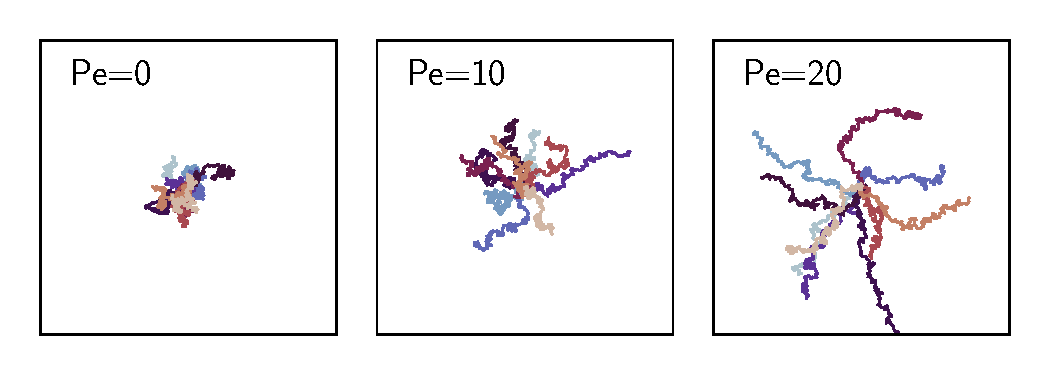
\includegraphics[width=\linewidth]{active-trajs}
  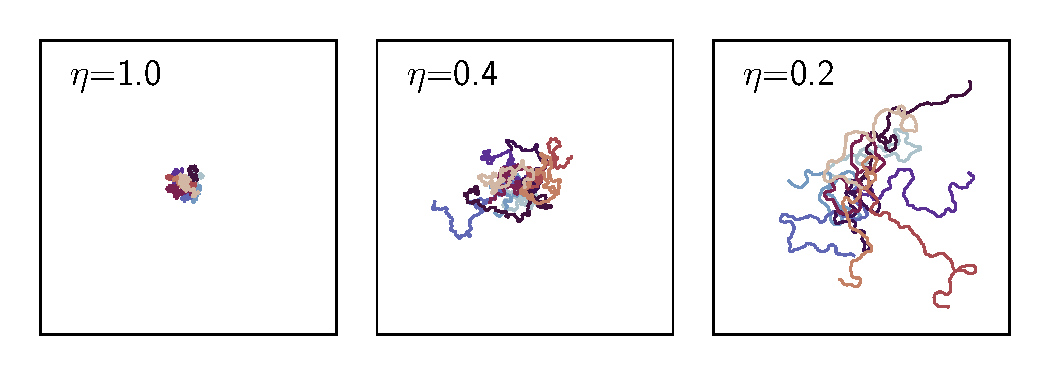
\includegraphics[width=\linewidth]{vicsek-trajs}
  \caption[Trajectories of Active Particles]{
  Trajectories of Active Particles.
  Top: the trajectories of active Brownian particles (ABP) with different Péclet numbers (Pe).
  Bottom: the trajectories of Vicsek agents with different noise ($\eta$) values. 
  Each subplot presents the simulated trajectories of 10 particles.
  }
\label{fig:active-trajs}
\end{SCfigure}


An alternative way to keep track of the activity, is to specify the randomness directly. For instance, we could rotate the moving direction of the active particles randomly, to interrupt their otherwise ballistic self-propelling movement. A system with large noise value therefore would have a low Pe number, hence low activity.
The effect of the noise is shown in Fig.~\ref{fig:active-trajs}. When $\eta = 1$, the rotation is totally random, corresponding to the situation when $\mathrm{Pe}=0$. By reducing the noise, the particles explore more spaces, being more active.\marginfootnote{
It is important to emphasise that the noise term $\eta$ is exclusively used for the Vicsek model, without being referred to as the activity.
}



\subsection{What does active matter do?}
\label{section:active-phase}


The reason we focus on the two aspects of the activity, is related to the two famous models for the active matter. One of the model is the active Brownian particles (\gls{ABP}), where the active particles interact with each other via a short-ranged repulsive interaction. The activity of the active Brownian particles is often represented by the Péclet number \cite{romanczuk2012, mauleon-amieva2020, turci2021}. 
Another widely used model for active matter is the Vicsek model, where the active particles align their orientations with nearby neighbours. The activity of particles in the Vicsek model is often controlled by the noise term \gls{eta} \cite{vicsek1995, gregoire2004, pimentel2008}.

These two models revealed two important phase\marginfootnote{
We committed to follow \citeauthor{toner2005}, calling the \emph{non-equilibrium steady state} with an underlying symmetry a ``phase''.
In the active matter community, this usage of the term ``phase'' is widely accepted.
} behaviours of active matter, which are summarised in Fig.~\ref{fig:active-phase}. 
It is important to stress that the two phase diagrams are sketched in a qualitative way, and some details are ignored. Nevertheless, the phase diagrams are consistent with simulations results, for both 2D and 3D systems \cite{stenhammar2014, turci2021, vicsek1995, solon2015, chate2020}.


\begin{SCfigure}
  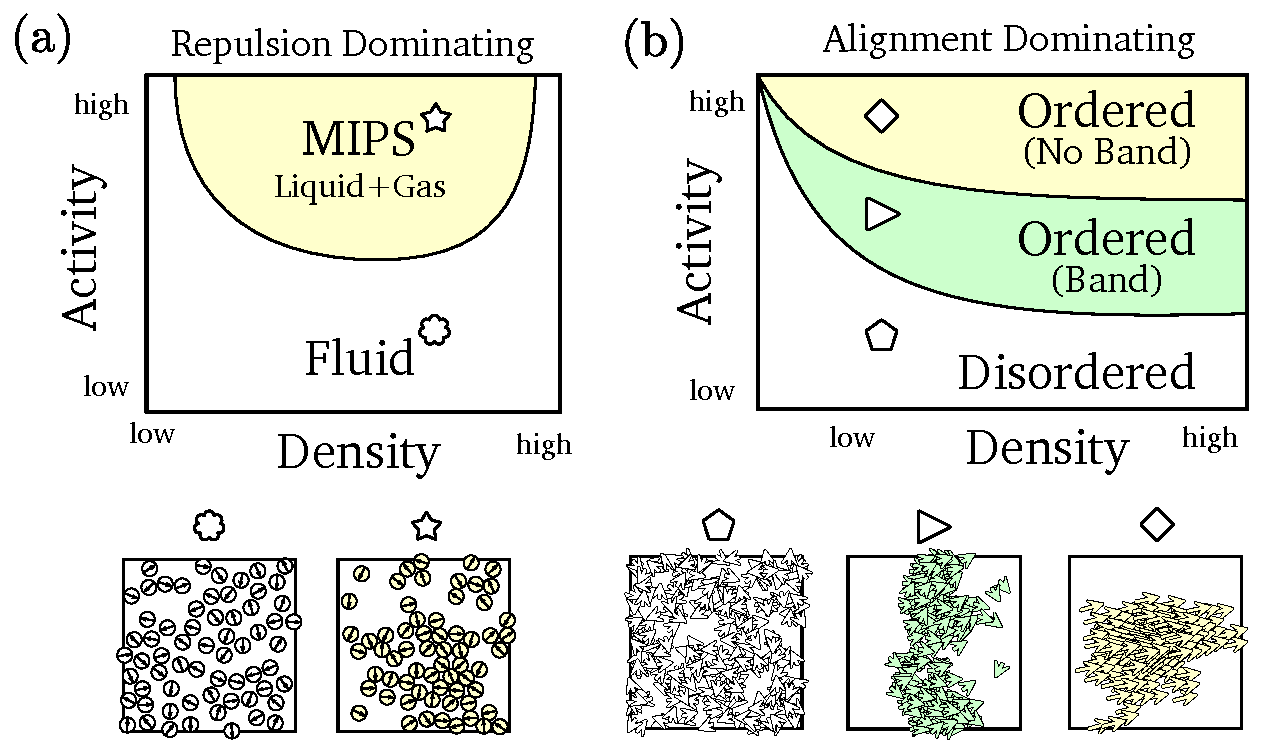
\includegraphics[width=\linewidth]{active-phase}
  \caption[Common phase diagrams of active matter]{
  Two types of common phase diagrams of active matter.
  (a) The phase diagram of active matter systems where the short-range repulsive interaction is dominating. These systems exhibit liquid-gas separation at high level of activity.
  (b) The phase diagram of active matter systems where the velocity-alignment interaction is dominating. These systems exhibit a flocking transition at high activity levels and large density values.
  }
\label{fig:active-phase}
\end{SCfigure}


For the active matter system whose interaction is dominated by short-range repulsion, its behaviour can be summarised in Fig.~\ref{fig:active-phase} (a). While the activity is low, the system forms a fluid with a uniform density distribution, like the behaviour of hard disks (in 2D) \cite{krauth2006, klamser2018, stenhammar2014} or hard spheres (in 3D) \cite{stenhammar2014, robinson2019, turci2021}. 
With high activity values, the active particles begin to phase separate into high density ``liquid'' and low density ``gas'', a phenomena known as the \emph{mobility induced phase separation} (\gls{MIPS}) \cite{fily2012, cates2015, digregorio2018, turci2021}. MIPS is reminiscent of the liquid-gas coexistence in equilibrium systems with attractive interactions \cite{hansen1969, speck2016, anderson2017}. This similarity is indeed surprising: the activity seems to cause an effective attraction between particles \cite{turci2021}. The apparent attractive interaction could be explained by a feedback loop, where the active particles slows down when they accumulate, and the slowing down also induces accumulation of more particles \cite{cates2015}.

On the other hand, for active particles that align their orientation with nearby neighbours, instead of repel each other, their phase behaviour could be summarised in Fig.~\ref{fig:active-phase} (b). In the low activity and low density region, the particles perform disordered movements like the ideal gas. However, with increasing activity and density, the system would undergo an order-disorder transition\marginfootnote{
The transition is also called the \emph{flocking transition} in some literatures \cite{cavagna2020, kürsten2021}. The phenomena where particles perform ordered movement is sometimes called flocking \cite{toner1995, ginelli2010}.
}, where all the particles would share the same moving direction, with slight perturbations from the rotational noise \cite{vicsek1995, solon2015}.
The ordered phase in Fig.~\ref{fig:active-phase} (b) could further be divided into two distinct kinds. When the activity is moderate, the active particles ``travel in bands'' \cite{chate2008}, featuring dense stripes separated by dilute regions, as shown in Fig.~\ref{fig:active-phase} ($\triangleright$). With high activity, the particles do not travel in bands, but rather form a coherent cluster, shown in Fig.~\ref{fig:active-phase} ($\diamond$). The banding phase is an important structural feature of active matter with alignment interactions, which is observed in colloidal experiments \cite{bricard2013, geyer2018, mauleon-amieva2020}.


There are more types of interactions beyond repulsion and alignment. Active matter with more complex interactions exhibits rich behaviours.
For instance, the incorporation of pairwise alignment, short-ranged repulsion, and long-ranged attraction leads to a complex phase behaviour including the fluid, the moving crystal, as well as the polar bands \cite{mauleon-amieva2020}.
The combination of short-ranged repulsion, and dipole-dipole interaction coupled with an alternating current electric field leads to the formation of labyrinth-like patterns \cite{sakai2020}.
In addition, the vision-based acceleration could lead to the formation of a cohesive cluster \cite{lavergne2019}, as a new mechanism beyond of pairwise attraction and MIPS.


It is important to point out that there are topics of active matter that are not covered in this section. For instance, we did not discuss the apolar active matter with nematic alignment interaction \cite{narayan2007, chate2020, bar2020}.
In addition, the effect of activity on the crystallisation \cite{moore2021, omar2021, klamser2018} and glass transition \cite{berthier2017, klongvessa2019} is not discussed.
We also downplayed the importance of dimensionality, which changed the phase diagram of significantly \cite{omar2021, speck2022}.

Finally, we want to specify the meaning following terms, because they were originally developed in equilibrium statistical mechanics. And applying these terms for active matter could cause confusion.

\begin{tcolorbox}[
enlarge bottom by=0.5em,
enlarge top by=0.5em,
]

\begin{description}
	\item [Phase] \hfill \\
	The non-equilibrium steady state with an underlying symmetry, for systems in the thermodynamic limit where the number of particles $\rightarrow \infty$.
	\item [Microscopic State] \hfill \\ Here we refer to the locations, velocities, and orientations of all the active particles. 
	\item [Macroscopic State] \hfill \\ Here we refer to a few global variables, like the density and activity, for an active matter system.
	\item [Collective] \hfill \\ We use the term to specify the property exhibited by a group of animals, in contrast to the property exhibited by individuals.
	\item [Collective Behaviour] \hfill \\ The macroscopic states exhibited by an active matter system.
	\item [Collective Motion] \hfill \\ The microscopic states of an active matter system.\marginfootnote{For a group of fish, we can directly observe their collective motion, and study their collective behaviour by further analysis.}
\end{description}

\end{tcolorbox}

\noindent It is notable that the meaning of these terms is different in different fields. But they will be consistent in this thesis.

\subsection{Animals as Active Matter}

A group of animals is a typical active matter system, as each individual spends their energy to perform movement \cite{ramaswamy2017}.
Consequentially, the two typical phase behaviour of active matter, presented in Fig.~\ref{fig:active-phase}, has been observed in animal groups.
For instance, the MIPS-like behaviour, where a dilute region and a dense region coexist, was observed in a group of beetles \cite{devereux2021}.
In addition, European Starlings exhibit ordered movement \cite{cavagna2010}, while the midges exhibits the disordered movement \cite{attanasi2014pcb}. From a group of zebrafish, we also observed the order-disorder transition \cite{yang2021pcb}, which will be discussed in chapter~\ref{chapter:fish_analysis}.


There is an implicit paradigm to study the active matter system in the scientific community \cite{allen2017}, which includes three steps. Firstly we observe the behaviour of real animals and calculate their behavioural features. Then we simplify the animals with a mathematical model that captured all the essential features. Finally we study the model either numerically or analytically, to have a comprehensive understanding. An example of this approach, was recently demonstrated by \citeauthor{bull2021ep3} with a trilogy\marginfootnote{
The authors explained their work in a serious of helpful tweets \cite{prakash2021}. A tweet is a text snippet people posted on a website named ``Twitter''.
}
on the movement of cilia \cite{bull2021ep1, bull2021ep2, bull2021ep3}. It is important to stress that the research on active matter does not always follow the order of ``observation, model, and theory'', even though we will review the literature in such order.


\section{The Observation of Animal Behaviour}
\label{section:intro-observe}

Observing the collective motion of animals is a visually pleasing task, since a group of animals could from striking patterns in nature \cite{vicsek2012}. 
It is expected that animals could do more interesting things, compared with the behaviour of simple active matter systems introduced in section~\ref{section:active-phase}. This is because the interaction between the animal individuals is based on vision \cite{strandburg-peshkin2013}, sound \cite{ota2020}, and smell \cite{miller2022}. All of these biological sensors makes the interaction of animals being more complex than a combination of repulsion and the velocity alignment.

\subsection {Complex Patterns Seen in Nature}

Even the visual footages of the animal behaviour, like the photos and the videos, are useful information.
For instance, the early active matter models were aiming at simulating the movement of animals with visual similarity, rather than quantitative agreement \cite{reynolds1987, vicsek1995, couzin2002}.
Two typical complex patterns commonly seen in the nature were presented in Fig.~\ref{fig:animals}. The first kind is flocking birds, which from a coherent cluster with a smooth but irregular shape (Fig.~\ref{fig:animals}, left subfigure). Another kind of pattern were formed by a school of fish, where the fish rotates around a common axis collectively (Fig.~\ref{fig:animals}, right subfigure), exhibiting a ``milling'' behaviour.

\begin{SCfigure}
  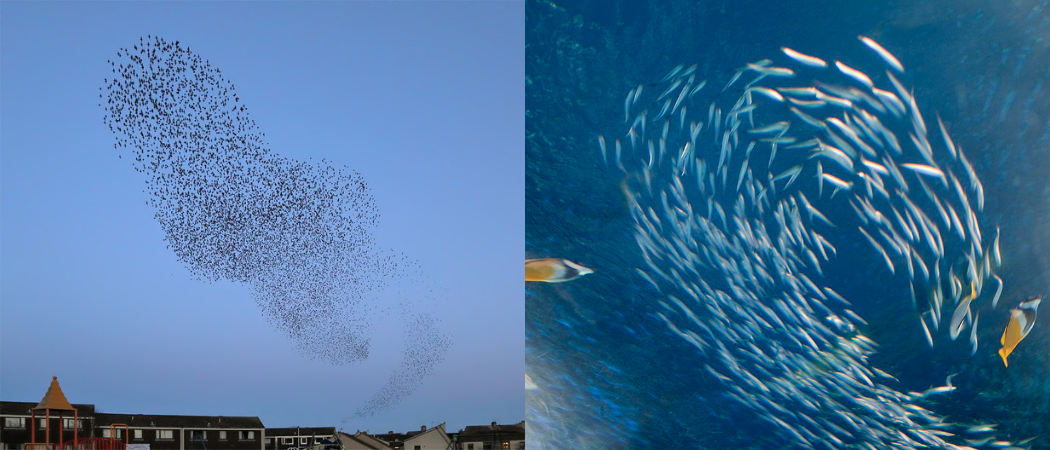
\includegraphics[width=\linewidth]{animals}
  \caption[Complex patterns formed by animals]{
  Photos of complex patterns formed by animals. Both photos were distributed under the Creative Commons Licence.
  Left: the murmuration of flocking European starlings. Each dark dot represents a bird. The photo was taken by \href{https://www.geograph.org.uk/photo/6389346}{Walter Baxter} in Eyemouth, Scotland.
  Right: a school of prey fish forming a circle, as a defensive move against two nearby butterfly fish. The photo was taken by an Internet user named ``\href{http://www.freeimageslive.co.uk/free_stock_image/butterfly-fish-jpg}{lifefish}'', a semi-pro photographer.
  }
  \label{fig:animals}
\end{SCfigure}

\subsection{Observing the Collective Motion in 2D}

To understand the animal behaviour in more detail, it is important to go beyond the visual inspection, and perform quantitative measurement.
One popular option to study animal behaviour is to analyse videos, recorded with conventional cameras, which capture the movement of animals in 2D.
Both the flocking behaviour and the milling behaviour, shown in Fig.~\ref{fig:animals}, were observed from these 2D videos.
For examples, there are analyses on the behaviour of locusts \cite{buhl2006, yates2009}, fish \cite{becco2006, fontaine2008, puckett2018, macgregor2020}, penguins \cite{gerum2013, gerum2018}, and many other animal species \cite{mersch2013, feinerman2018, mendez-valderrama2018, ginelli2015pnas}.


As a well developed experimental technique, the 2D tracking of animals is an easy task. There are multiple free and user-friendly softwares available online, enabling researchers to carry out 2D tracking tasks \cite{perez-escudero2014, rodriguez2017, romero-ferrero2019, walter2021}. The performances of various tracking softwares were quantified in a recent comprehensive review \cite{panadeiro2021}.
In addition to cameras, there are alternative technologies for the study of animal behaviour. For instance, \citeauthor{makris2006} used a waveguide remote-sensing technology to record the density distribution of fish shoals at the scale of kilometers \cite{makris2006, makris2009}.
The GPS is also another option to tag individual animals, and obtain trajectories \cite{papageorgiou2020}.
%For some animals, it is also possible to tag them with informative markers \cite{webster2009, mersch2013, jolles2017}.


\subsection{Observing the Collective Motion in 3D}

The idea of tracking the movement of animals in 3D, with the help of cameras, was proposed early in the 1960s \cite{cullen1965, pitcher1973}.
The fundamental principles to carry 3D tracking were covered by the multiple view geometry in the computer vision community \cite{hartley2003}. Very briefly, the picture in one 2D image offered two constraints on the 3D coordinates of an object. Therefore, 3D coordinates can be determined with images from two or more cameras \cite{cavagna2008ab}. Figure~\ref{fig:locate3d-cartoon} sketched an example for this idea.

\marginpar{
\centering
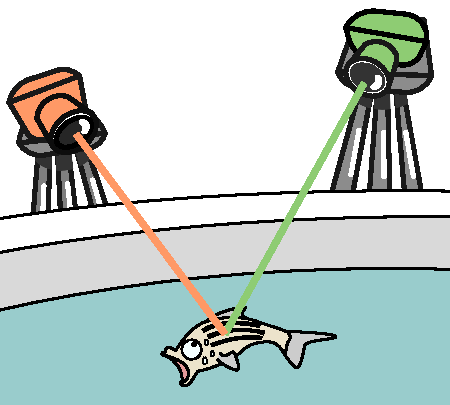
\includegraphics[width=\marginparwidth]{locate3d-cartoon}
\captionof{figure}[Locating a zebrafish in 3D]{
	Schematic illustration for locating a zebrafish in 3D with two cameras. 
}
\label{fig:locate3d-cartoon}
}


Even though the idea is simple, setting up a 3D tracking experiment and obtaining long trajectories of multiple animals are still challenging \cite{pedersen2020}.
Multiple new algorithms have been proposed to tackle the various issues during the tracking process. These issues includes the calibration of camera during field study \cite{cavagna2008ab, ling2018}, the visual occlusions where two animals overlap in the image \cite{cavagna2021ieee}, the ambiguity for the stereo matching of trajectories in multiple views \cite{attanasi2015b}, and the recovery of identity information given the coordinates in different time points \cite{ouellette2005ef, xu2008}.

Despite the technical challenges, the 3D tracking of birds \cite{cavagna2008ab, nagy2010, attanasi2014np, ling2019nee}, insects \cite{butail2011, straw2011, attanasi2014prl, kelley2013, vandervaart2019}, as well as fish \cite{stowers2017, rosa2020, yang2021pcb} were reported.
For the birds, the order ``flocking'' phenomena were observed in \cite{ballerini2008pnas, cavagna2010, nagy2010, ling2018}. For the midges and the fish, the observed movements were disordered \cite{attanasi2014pcb, kelley2013, yang2021pcb}.

There are still two major technical challenges for the 3D animal tracking problem. Firstly, it is very hard to track a large flock of birds for a long time, because the flock would move outside the view of the cameras quickly. This is the reason some of the large scale statistical analysis are only performed on midges \cite{cavagna2017np}, rather than the birds\marginfootnote{
	I was told that the lack of long trajectory is the reason why the author of \cite{cavagna2017np} chose midges over birds.
}.
There is a recent breakthrough to track birds for a long period of time, by moving the cameras in a synchronised fashion \cite{cavagna2021}, but no experimental results were reported from the new system so far.
Another challenge is the 3D tracking of a large school of fish in the sea, which requires underwater equipments. In fact, there is still no quantitative field observation for the a large amount of fish in the milling phase, like those in Fig.~\ref{fig:animals}. Recently, the underwater 3D tracking methods were being developed \cite{francisco2020me, engel2021}, but only for fish groups with small sizes ($N < 10$).


\section{The Analysis of the Collective Motion}
\label{section:intro-analysis}


Analysing the animal movement involves two major steps. 
Firstly, we need to identify the different kinds of behavioural patterns of the animals, and assign the patterns to different phases. For patterns in a particular phase, we can study its feature with different correlation functions.

\subsection{Identifying Behavioural Patterns with \emph{Order Parameters}}
\label{section:intro-order}

This classification of different phases is important, because different phases have different properties.
We can use an \emph{order parameter}, which indicates the breaking of one kind of symmetry \cite{sethna2006}, to identify different phases. For instance, we could define the vector sum of the orientation of each individual as a order parameter ($\mathbf{P}$) \cite{vicsek1995}:

\begin{equation}
	\mathbf{P} = \frac1N \sum_i^N \mathbf{o}_i
\label{eq:pol}
\end{equation}

\noindent where $\mathbf{o}_i$ is the orientation of the $i$th individual in a group with \gls{N} members. We use symbol \gls{pol} to represent the norm of the vector \gls{polvec}. For a very large group, the value of $\Phi$ would approach zero if the orientations of the individuals were completely de-correlated. On the other hand, the value of $\Phi$ would tend to unity if all the individuals have the same orientation. In the latter case, the rotational symmetry is broken because the group has one single moving direction, where the vector $\mathbf{P}$ is pointing at.
The order-disorder transition in Fig.~\ref{fig:active-phase} (b) is characterised by a discontinuous change of $\Phi$. For a flock of birds moving towards the same direction, the value of $\Phi \sim 1$ \cite{attanasi2014np}. For a swarm of randomly moving midges, the value of $\Phi \sim 0$ \cite{attanasi2014pcb}.

\marginpar{
\centering
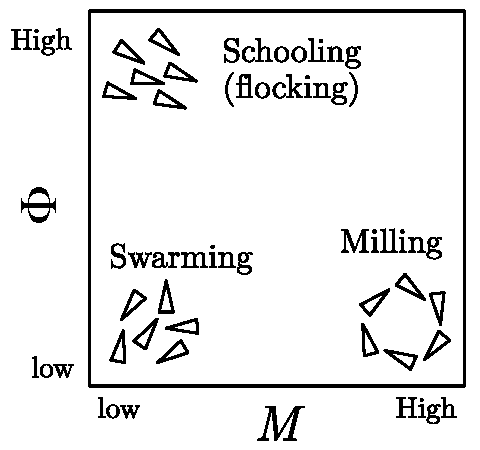
\includegraphics[width=\marginparwidth]{phase-fish}
\captionof{figure}[Different phases revealed by two order parameters.]{
	The schooling, milling, and swarming phases described by  two order parameters. The parameter $\Phi$ indicates the degree of synchronised movement, while the parameter $M$ indicates the existence of collective rotation.
}
\label{fig:phase-fish}
}

The milling behaviour of the fish, shown in Fig.~\ref{fig:animals}, needs a different order parameter that focuses on the angular momentum of each fish. This order parameter is written as,

\begin{equation*}
	\mathbf{M} = \frac1N \sum_i \left(
		\mathbf{o}_i \times \frac{
			\mathbf{r}_i - \mathbf{c}
		}{\vert \mathbf{r}_i - \mathbf{c} \vert}
	\right)
\end{equation*}

\noindent where $\mathbf{r}_i$ represent the location of the $i$th individual, and \gls{center} represents the location of the group centre. Again, we use the symbol \gls{mill} to represent the norm of \gls{millvec}. For a group of fish that are rotating around a common axis, the value of $M$ would be close to one \cite{couzin2002, calovi2014}. For the system that does not perform the collective rotation, the value of $M$ would approach zero.

With the two order parameters, the behavioural pattern of the fish, as well as other species, could be categorised into the swarming, the milling, and the schooling phases, as shown in Fig.~\ref{fig:phase-fish}. The existence of these phases were observed in the a group of golden shiners (\emph{Notemigonus crysoleucas}) \cite{tunstrom2013}.
Operationally, establishing the order parameters helps the identification of the phase that the experimental data (or simulation results) belongs to, without visual inspection.

Inside each phase, we could study its feature by examining the \emph{correlations} in the time and in the space \cite{grigera2020}. The spatial correlations gives us information about the structure of the animal group, while the temporal correlations reveals the dynamics of the system.


\subsection{Probing the Structure: the Radial Distribution Function}
\label{section:intro-corr-rdf}

The radial distribution function (\gls{RDF})\marginfootnote{
The radial distribution function is also named \gls{gr}, which is read as the ``g of r''. We use the term RDF and $g(r)$ interchangeably in this thesis.
} can be used to reveal the structure of the animal group. An example of the RDF, also known as the $g(r)$, is shown in Fig.~\ref{fig:corr-examples} (d). This RDF probes the structural features of a system shown in Fig.~\ref{fig:corr-examples}(a). The value of $g(r)$ at very short range is zero, which represents the short ranged repulsion. The location of the peak of the $g(r)$ is a proxy to the nearest neighbour distance, while the height of the peak indicate the cohesiveness of the group \cite{hansen2013}. The slow decay in Fig.~\ref{fig:corr-examples} shows the presence of large clusters in Fig.~\ref{fig:corr-examples}(a).
The size of these large clusters can be captured by the $r$ value when $g(r)$ decays to zero. This distance value is called \emph{correlation length} of the density \gls{xirho}. 

Notably, the RDF is an important tool for the study of the fluid in equilibrium, because it determines the thermodynamic behaviour of the system \cite{pathria2011, hansen2013}. For instance, the internal energy, the pressure, and the compressibility can be calculated from $g(r)$. However, this validity does not hold for animal groups due to their non-equilibrium nature\marginfootnote{
Recent study suggested that the $g(r)$ can be used to calculate the compressibility for active Brownian particles \cite{dulaney2021}.
}. Nevertheless, the RDF is still a very useful tool to characterise the structure of animal groups, which had been  applied to study the fruit flies \cite{mendez-valderrama2018}, birds \cite{cavagna2008}, the fish \cite{romenskyy2017}, and the penguins \cite{gerum2018}.

Finally it should be mentioned that the $g(r)$ is a two point correlation function, which is not aware of the possible many-body correlations. It was recently revealed by \citeauthor{kursten2020} that higher order correlations are important for the alignment dominating system \cite{kursten2020}, typically the ordered phase in Fig.~\ref{fig:active-phase} (b). The measurements of higher order correlation functions is rare in the study of animal behaviours, but the tools are available in the studies of liquid \cite{zahn2003, williams2007, hallett2020}.
Biologically, the existence of high order structure would be expected. For instance, the formation of the typical V-shape pattern \cite{Hayakawa2013} for a flock of geese could not emerge as a result of simple pairwise interaction.


\begin{SCfigure}
  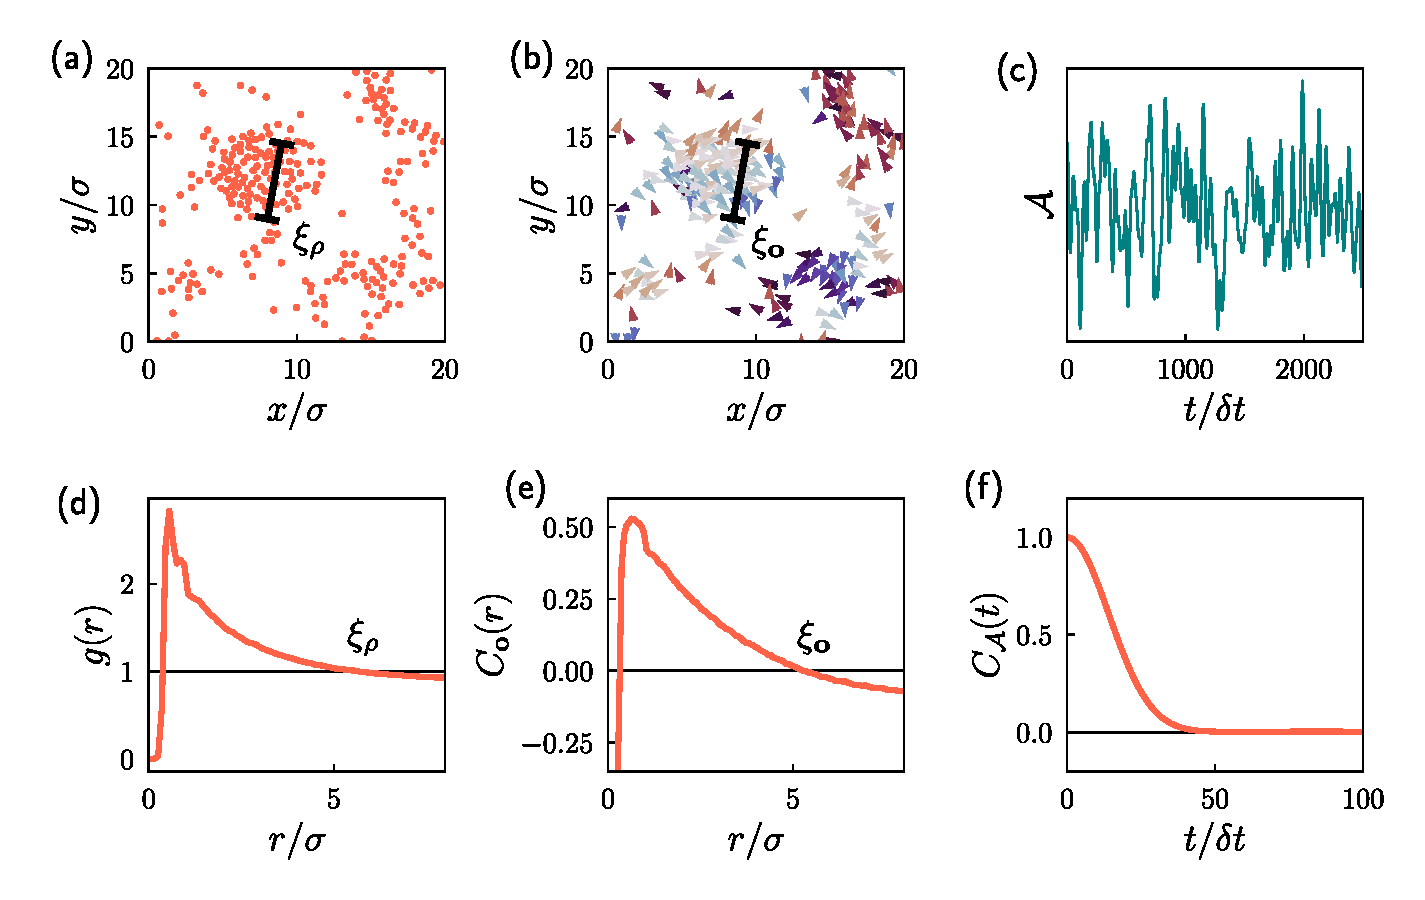
\includegraphics[width=\linewidth]{correlations}
  \caption[Examples of common correlation functions]{
  Examples of common correlation functions and the structure/dynamics that they probe.
  (a) The coordinates of 256 particles with short-ranged repulsion and alignment interaction.
  (b) The orientation of the particles in (a) represented as arrows located at their corresponding coordinates.
  (c) A time series signal of quantity $\mathcal{A}$.
  (d) The radial distribution function ($g(r)$) calculated from the model that generated (a) and (b).
  (e) The connected correlation function of the orientations of particles calculated from the model that generated (a) and (b).
  (f) The auto-correlation function of the signal shown in (c).
  }
  \label{fig:corr-examples}
\end{SCfigure}


\begin{tcolorbox}[
title=Implicit Assumption of the Pairwise Distance $r$,
enlarge bottom by=0.5em,
enlarge top by=0.5em,
]
Using the scalar variable $r$ in a correlation function, we implicitly assumed two conditions. Firstly, the interaction of two particles only depends on their relative distance. In other words, the interaction should be spherically symmetrical. In addition, we assume the system is isotropic with translational symmetry. Therefore, shifting two particles together would not affect their interaction. Without these assumptions, the correlation should be changed from $g(r)$ or \gls{cr} to $g(\mathbf{r}_1, \mathbf{r}_2)$ or $C(\mathbf{r}_1, \mathbf{r}_2)$.
\end{tcolorbox}



\subsection{Probing the Dynamics: the Correlation function of Orientation}
\label{section:intro-corr-cvv}

For a group of animals, as well as other active matter systems, their dynamical features are important. To characterise the dynamics, we can calculate the correlation of the orientations (\gls{o}) of each animal at different distances (\gls{r}). An example of such a correlation function, \gls{cor}, is shown in Fig.~\ref{fig:corr-examples} (e), which characterised the local alignment of particles in Fig.~\ref{fig:corr-examples} (b). These particles are shown to align with nearby neighbours, exhibiting a positive value in the correlation value at short distances. 
%The alignment interaction is short ranged ($= 2\sigma$, where $\sigma$ is the space unit), but it triggered long range correlation, as 
The correlation function reaches 0 at a distance $\approx 5 \sigma$, corresponding to the correlation length of orientation ($\xi_\mathbf{o} = 5\sigma$).
If we compare the correlation functions from both Fig.~\ref{fig:corr-examples} (d) and (e), it is obvious that the two correlation lengths, $\xi_\rho$ and \gls{xio}, are similar. This means the large clusters in Fig.~\ref{fig:corr-examples} (a) and (b) move together, thanks to the local alignment of particles which leads to effective attraction.

Orientational correlation functions are widely applied in the study of animal behaviour, particularly for systems where alignment is the dominating interaction. For instance, the orientational correlation functions of midges \cite{attanasi2014pcb, ni2015epj}, fish \cite{yang2021pcb}, and birds \cite{cavagna2010} have been  reported, presenting short or long ranged orientational correlations.

This function is important also because its integral, $\int C_\mathbf{o}(r) dr$, is related to the \emph{susceptibility} (\gls{chi}) of the animal orientation under an external perturbation, under two assumptions. Firstly, the alignment interaction should dominate the animal behaviour, so that the energy\marginfootnote{
The energy ($E: \mathbb{R}^{N \times d} \rightarrow \mathbb{R}$) is a function that maps the \gls{dim} dimensional orientations of $N$ individuals to a probability weight. It is more likely to observe an animal group with low energy.\\
Notice the similarity of Eq.~\ref{eq:spin-energy} to the energy function (the \emph{Hamiltonian}) to those in magnetic systems, for instance the Ising model and the spin glass \cite{castellani2005, herbut2007}.
} of the system \gls{e} follows,

\begin{equation}
	E = -\sum_{i, j}{J_{ij} (\mathbf{o}_i \cdot \mathbf{o}_j})	- 
	h \sum_i{\mathbf{o}_i}
\label{eq:spin-energy}
\end{equation}

\noindent where $\mathbf{o}_i$ is the orientation of the $i$th member in the group, \gls{jij} is a coupling constant for a pair of member $i$ and member $j$, and \gls{h} represents the effect of an external field affecting the individuals' orientations. With the energy term, it is further assumed that the system is in equilibrium, where the entropy is maximised \cite{bialek2011}, so that the probability of the system in a microscopic state with energy $E$ is,

\begin{equation*}
	P(E) = \frac{\exp(-\beta E)}{\int \exp(-\beta E)},
\end{equation*}

\noindent where the integral in the denominator yields the \emph{partition function} of the system. These two assumptions ignored many biological details of the animals, but were confirmed to fit the experimental data \cite{bialek2011}.

Acknowledging the two discussed assumptions, the relationship between $C_\mathbf{o}(r)$ and $\chi = \langle \partial \Phi / \partial h \rangle$ can be derived with the linear response theory\marginfootnote{
	The susceptibility can also be obtained from the fluctuations of the polarisation order parameter ($\vert \mathbf{P} \vert$). Practically, estimating the susceptibility with $\int C_\mathbf{o}(r) dr$ is better for experimental data, because this route suffers less from measurement error and finite trajectory length \cite{attanasi2014prl}.
} \cite{herbut2007, attanasi2014pcb}. The susceptibility is biologically important, because it could be related to the ability of each individuals to change their moving direction, under the influence of a predator (which generates the field $h$ in Eq.~\ref{eq:spin-energy}). And it is been utilised in the study of midges by different research groups \cite{attanasi2014pcb, vandervaart2020}.

\subsection{Probing the Dynamics: the Auto-Correlation Function}
\label{section:intro-corr-acf}

Another way to probe the dynamics of the system is to calculate  the auto-correlation\marginfootnote{
The prefix ``auto'' comes from Greek word autos, which means ``self'' \cite{ben2020}.
} function (\gls{ACF}).
We use the notation \gls{cat} for the ACF for quantity $\mathcal{A}$, whose value typically fluctuates at different time points, like the signal in Fig.~\ref{fig:corr-examples} (c).
The corresponding $C_\mathcal{A}(t)$ is shown in Fig.~\ref{fig:corr-examples} (f), which decays from one to zero. The value of $C_\mathcal{A}(t)$ indicates the average similarity of the signal to itself after some lag time \gls{t}.
The auto-correlation function in Fig.~\ref{fig:corr-examples} (f) indicates that the system forgets its microscopic state, characterised by $\mathcal{A}$, after 50 $\delta t$ (the time unit).
This timescale is called the \emph{relaxation time}, noted by \gls{taua}. Knowing the values of relaxation time for different features let us grasp the dynamics of the system, typically for the identification of fast process and slow process. For instance, the orientational relaxation time of the fruit flies \cite{mendez-valderrama2018} and fish \cite{partridge1981, mwaffo2015, zienkiewicz2015} were estimated from the ACFs.

Beyond the determination of relaxation time, the ACF is important because its integral relates to the transport coefficient, a relation known as the Green-Kubo formula \cite{allen2017, pavliotis2014}. For instance, the integral of the ACF of the velocity (\gls{v}), $\int C_\mathbf{v}(t) dt$ yields the diffusion coefficient. However, this relation requires the collective motion of the animals, treated as a stochastic process, to be second-order stationary, where the ACF does not change with time. In chapter~\ref{chapter:fish_analysis}, we will see that this assumption is not true for the fish, as the \gls{cot} of 50 zebrafish changes with time.


\subsection{Novel Correlation Functions for Animals}
\label{section:intro-corr-special}


It is possible to craft novel correlation functions, like the $g(r)$, to study the structural features of animal groups. For example, \citeauthor{ballerini2008pnas} studied the distribution anisotropy of the neighbours of each bird in a group of European starlings \cite{ballerini2008pnas}. This anisotropy factor, noted as \gls{gamma} in \cite{ballerini2008pnas}, could be used to construct a correlation function $C_\gamma(n)$, with different neighbours rank\marginfootnote{
	For a bird, its nearest neighbour has the rank 1, the next nearest neighbour has the rank 2.
}  (\gls{nr}) values, shown in Fig.~\ref{fig:corr-animal}(a). This function \gls{cgamman} presents the decay of $\gamma$ with increasing $n$ values, and leads to a remarkable conclusion: a bird in a flocking group interacts with 7 neighbours on average \cite{ballerini2008pnas, cavagna2014}, regardless of its distances to these neighbours.
This behavioural feature is called a \emph{topological} interaction, as opposed to a metric interaction based on physical distances. This special correlation function was also used by \citeauthor{ling2019nc} to study the changing behavioural rules of jackdaw flocks \cite{ling2019nc}.


\begin{SCfigure}
  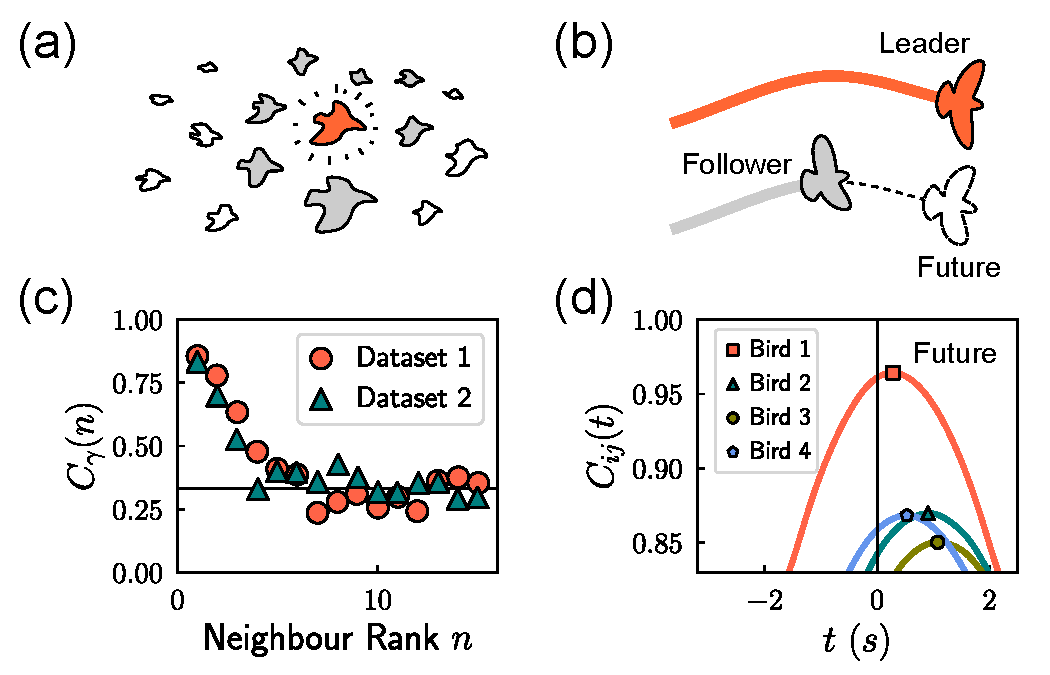
\includegraphics[width=\linewidth]{corr-animal}
  \caption[Examples of special correlation functions to characterise animals]{
Examples of special correlation functions to characterise animals.
  (a) The illustration of a topological interaction, where a highlighted focal bird interact with 7 nearby neighbours, regardless of the distances. This topological interaction is supported by correlation function $C_\gamma(n)$.
  (b) The sketch of a leading bird and a following bird. The following bird will align with the leader, after a short lag time. The leadership is supported by correlation function $C_{ij}(t)$.
  (c) The anisotropy correlation function $C_\gamma(n)$ of the European starlings. The data was obtained from \cite{ballerini2008pnas}.
  (d) The orientational cross-correlation function $C_{ij}(t)$ between a pigeon and its group members. The data was obtained from \cite{nagy2010}.
  }
  \label{fig:corr-animal}
\end{SCfigure}

The orientational cross-correlation function \gls{cijt} is another tool to study animals, proposed by \citeauthor{nagy2010} \cite{nagy2010}. It is essentially the correlation between the orientations of two individuals (labelled by $i$ and $j$) in time. Such function revealed the leader-follower relationship among the individuals in the group. An example is plotted in Fig.~\ref{fig:corr-animal} (b), where a following bird would try to align its orientation to a leader. Because of the behavioural inertia of the birds, there will be a slight lag time, for the follower to adjust its orientation. In other words, the follower will try to align with the leader ``now'', but the alignment is not instantaneous, and it could only happen in the ``future''. This lag time could be captured by the orientational cross-correlation function

\begin{equation}
	C_{ij}(t) = \langle
		\mathbf{o}_{i}(\tau) \cdot \mathbf{o}_{j}(\tau + t)
	\rangle,
\end{equation}

\noindent where the angular brackets $\langle \dots \rangle$ represents a time average. Examples of such cross-correlation functions, calculated from pigeons, are shown in Fig.~\ref{fig:corr-animal} (d). For a leading bird, the cross-correlation with its follower would lead to a peak at $t > 0$, because the follower's alignment would happen in the future. This leader-follower relationship of pigeons was also observed by \citeauthor{chen2015epj} \cite{chen2015epj}. And this correlation function as used by \citeauthor{yomosa2013} for the study of gulls \cite{yomosa2013}.

Finally, we want to mention a recent method to quantify the hidden order \cite{martiniani2019prx}, and its correlation length \cite{martiniani2020}. This method used the compression algorithm in computer science to quantify the entropy, as the information with high entropy could not be compressed effectively \cite{mcanlis2016}. This method was demonstrated to be useful for the study of both kind of active matter systems in Fig.~\ref{fig:active-phase} \cite{martiniani2019prx, cavagna2020}.


\section{Understanding the Animal Behaviour}
\label{section:intro-model-theory}

The order parameters, and the correlations calculated from a group of animal can be used to construct mathematical models. These models can be studied numerically or analytically, to make predictive conclusions about the animal behaviour.


\subsection{Microscopic Approach: Agent Based Models}

The most famous model in the active matter community is arguably the Vicsek model proposed by \citeauthor{vicsek1995} in 1995. The model assumed the individual animal in a group align with nearby neighbours. This alignment process is interrupted by the orientational noise ($\eta$ in Fig.~\ref{fig:active-trajs}).
The phase diagram in Fig.~\ref{fig:active-phase} (b) depicted the behaviour of the Vicsek model. The movement of active particles in the ordered phase is visually similar to the collective motion of birds shown in Fig.~\ref{fig:animals} \cite{ballerini2008}.

The Vicsek model is a very simple model, which often lack essential elements to reproduce the behaviour of animals accurately. For instance, the lack of inertia in the Vicsek model makes it incapable of describing the collective turning behaviour of European Starlings \cite{attanasi2014np}. To explain the experimental results, an inertial spin model \cite{attanasi2014np, cavagna2015} was proposed. In addition, the topological interaction rule \cite{ballerini2008pnas}, shown in Fig.~\ref{fig:corr-animal} (a), could also be added into the Vicsek model,  which supressed the travelling bands\marginfootnote{
The existence of the bands for the topological Vicsek model is still under scrutiny. Early results, both simulations and theories, suggested the absence of the band \cite{ginelli2010, chou2012, peshkov2012}. But recent simulations and theories suggested the existence of the band \cite{martin2021, rahmani2021}.
}.


The milling behaviour of the fish \cite{tunstrom2013}, shown in Fig.~\ref{fig:animals} was also modelled by \citeauthor{couzin2002} in early 2000s, known as the Couzin model. This proposed model includes a short ranged repulsion, with an alignment interaction in intermediate range, as well as a long-ranged attraction \cite{couzin2002}. All the phases introduced in Fig.~\ref{fig:phase-fish}, the schooling, milling, and the swarming, can be reproduced in the Couzin model \cite{tunstrom2013}. The same phases could also be reproduced in a model with topological interaction rules \cite{gautrais2012, calovi2014}, as well as a model with only local attraction interactions \cite{strombom2011}.




\subsection{Hydrodynamic Approach: Continuum Models}

One further step to understand the animal behaviour is to convert the microscopic description of the individuals, into large scale, \emph{hydrodynamic} models\marginfootnote{
Also known as the continuum models.
}. By doing so, we ignored the details of the particles, and treat the system as flowing liquid.
This approach is demonstrated by \citeauthor{toner1995}, who derived qualitative predictions for the large scale behaviour of active particles, from hydrodynamic equations.
Typically, these hydrodynamic equations describe the evolution of density field and the polarisation field ($\mathbf{P}$ in Eq.~\ref{eq:pol}), in the form of coupled partial differential equations \cite{toner1995, toner1998, shaebani2019}.
The hydrodynamic description of active matter are expected to recreate the result of the microscopic model at a large-scale \cite{mahault2019}.
The introduction of various continuum models is beyond the scope of this thesis, but we want to discuss some predictive conclusions from theoretical analysis of these models.

The major conclusion from \citeauthor{toner1995} in their early analysis is that the ordered phase discovered by \citeauthor{vicsek1995}, shown in Fig.~\ref{fig:active-phase} (b), exists in 2D. This confirmation is important because the ordered phase could not be proved by numerical simulation in the computer\marginfootnote{
The numerical simulation could generate misleading results, mainly due to the finite system size. For instance, a discontinuous phase transition in the thermodynamic limit ($N \rightarrow \infty$) might appear continuous in a small system ($N \sim 10^4$) \cite{vicsek1995, nagy2006, chate2008EPJ}.
}.
In addition, the analysis carried out by \citeauthor{mermin1966} \cite{mermin1966} explicitly ruled out the possibility for the long ranged order in 2D in equilibrium \cite{sethna2006, ginelli2016}.
In other words, the activity of particles in the Vicsek model is surprisingly crucial for the flocking phenomena.

Beyond the existence of the ordered phase in the 2D Vicsek model (Fig.~\ref{fig:active-phase}), the analysis of the continuum models also yields other useful results such as the scaling of velocity correlation function and the discontinuous nature of the order-disorder transition \cite{solon2015, martin2021}. However, as \citeauthor{ouellette2022} commented recently, it is challenging to link the continuum models to animal groups, especially to compare the theoretical prediction with experimental results, due to the lack of large scale experimental results \cite{ouellette2022}.


\subsection{Thermodynamic Approach: Equation of State}

It is also possible to take a \emph{thermodynamic} approach to study the animal behaviour. Thermodynamics is capable of describing the behaviour of equilibrium systems, whose underlying microscopic dynamics are unknown \cite{ouellette2022}.
For instance, the laws of thermodynamics were established and applied, long before the discovery of atoms and before the development of statistical mechanics \cite{sethna2006, ouellette2022}.
To do something conceptually similar, we will need to define some \emph{state variables}, which are conceptually similar to the pressure (\gls{press}), volume (\gls{vol}), temperature (\gls{temp}), entropy (\gls{entropy}), chemical potential (\gls{mu}) and particle number ($N$), to summarise the behaviour of animals.
If the animals were behaving in an equilibrated way, these state variables would be constrained, yielding an equation of state, that would be useful to develop predictive theories.

For instance, the \emph{virial equation}\marginfootnote{
Notice the law for the ideal gas is $PV = Nk_BT$.
} of an equilibrium system is

\begin{equation}
	 PV = Nk_BT + \langle \mathcal{W} \rangle
\label{eq:virial}
\end{equation}

\noindent where \gls{kb} is the Boltzmann constant, $\langle \dots \rangle$ denotes the time average, and \gls{pressint} is the internal pressure caused by the interaction of particles \cite{hansen2013ch2, allen2017}. Similar relation is observed in \cite{gorbonos2016} for a group of midges, which can be used to calculate the pressure $P$ exerted on the animals by the external field.
In addition, a small perturbation filed acted on the equilibrium system will cause a \emph{linear} response. This linear relationship is observed experimentally in \cite{ni2015prl}.
Further more, \citeauthor{sinhuber2017} were able to observe a constant chemical potential difference between dilute clusters and dense clusters in a swarm of midges, suggesting the existence of phase equilibrium\marginfootnote{
It is important to point out that the chemical potential in \cite{sinhuber2017} took a special definition from \cite{takatori2014}, which depends on the pressure. Again, the pressure in \cite{sinhuber2017} took another special definition, with underlying assumption that the midges were active particles without interaction, and were bounded together by an harmonic potential. Even though the definition of state variables are not very rigorous, their results are still surprising, which should not be discredited.
}.
Remarkably, their experimental results also suggest that detailed balance is maintained, for midges that switch between the two phases \cite{sinhuber2017}.
That is to say, the probability that one midge goes from a dilute region to a dense region, is equal to its counterpart for the reverse process. The detailed balance suggested an equilibrated behaviour of animals at large scale, even though the animal individuals are active and out of equilibrium. This ``regained equilibrium'' at large scales had also been reported from computer simulation \cite{egolf2000}.

Following this path, \citeauthor{sinhuber2021} presented a equation of state for midges, written as

\begin{equation}
	PV^{1.7} = c N T^2
\label{eq:eos-midge}
\end{equation}

\noindent where $c$ is a constant, while $P$ represents an effective pressure, $V$ represents the volume of the convex hull constructed from the animal coordinates, and $T$ represents the effective temperature that links to the second moment of the speed distribution.
Even though this equation contains quantities with heuristic definitions (the $P, V, T$ have special definitions), and fitting parameters obtained from experiments (the value of $c$, and some exponents), it  predicted the changing macroscopic states of midges under different perturbations successfully \cite{sinhuber2021}.

Even though the thermodynamic approach is capable of predicting the macroscopic behaviour the the animals, it is less used compared to other approaches, perhaps for the lack of consensus on the definition of the suitable thermodynamic state variables.
However, it is valuable also from a data science perspective, as a guide for us to project high dimensional data (the phase space) to a low dimensional feature space (the space spanned by few thermodynamic state variables). Such dimensional reduction analysis was also carried out manually \cite{yang2021pcb}, or with machine learning methods\cite{tang2020}, without the thermodynamic inspiration.

\section{Is Active Matter an \emph{Useful} Concept?}
\label{section:intro-benefit}

Physicists mention animals as typical active matter in the literatures \cite{reynolds1987, vicsek1995, chate2008EPJ, chen2015, kürsten2021}, but the biology community rarely acknowledges this perspective \cite{ouellette2022}, except for some ecology literatures \cite{guttal2012, tang2020}. The lack of mutual engagement is understandable, as it is difficult to apply the knowledge of active matter physics to biological topics. For instance, how does the activity affect the fitness of the animal group in a given environment? Would sick animals be less active in the wild? My fish is swimming strangely, does activity help to explain the data? To the best of my knowledge, the answers still remain elusive.

However, there are successful examples that bridge this gap between statistical physics and biology.
For instance, the observation and analysis on the European starlings revealed two unexpected features, the topological interaction \cite{ballerini2008pnas}, and the scale-free correlation \cite{cavagna2010}. These two findings are biological facts, even though their connection to the physiology is still missing \cite{ouellette2022}.

%By monitoring the movement of human bronchial epithelial cells (HBECs), typically their dynamical heterogeneity \cite{berthier2011}, \citeauthor{park2015} linked the (biological) mesenchymal-to-epithelial transition \cite{kalluri2009} to the (physical) unjamming-jamming transition \cite{park2015}. Such linkage is important, because the transition process leads to a collective cellular migration, that is closed related to wound repair, cancer invasion, and common diseases like asthma \cite{park2015}.

In chapter~\ref{chapter:fish_mutation} we will present another attempt, to reduce the gap between the biology and physics. 
Operationally, we studied the behaviour of the mutant fish, whose genetic modification is related to human diseases.
Using the correlation function introduced in section~\ref{section:intro-corr-acf}, we discovered the mutant fish are, surprisingly, more active.
We characterised the collective behaviour of the mutant fish with the order parameter introduced in section~\ref{section:intro-order}.
We then explained the behaviour of mutant fish with a microscopic active matter model, introduced in section~\ref{section:intro-model-theory}.
We hope this is an example that the active matter physics can be \emph{useful}.


\begin{adjustwidth}{0cm}{-5cm}

\begin{tcolorbox}[
fonttitle=\sffamily\Large,
right=0.1\linewidth,
top=5mm,
bottom=5mm,
title=Summary of Chapter 2,
]

\begin{itemize}
	\item We gave a brief introduction on active matter, featuring the following concepts.
	\begin{description}
		\item[Active Matter] \hfill \\ 
		A out-of-equilibrium system, containing active particles which constantly inject energy to the system.
		\item[Activity] \hfill \\ 
		The ratio of deterministic, self-propelling movement and the stochastic movement because of thermal fluctuation. We can increase the activity, by increasing the self-propelling speed, or by reducing the level of randomness.
		\item[Phase Behaviour] \hfill \\
		Active particles could exhibit different phase behaviours under different conditions, for instance the MIPS and the order-disorder transition.
	\end{description}
	\item We reviewed recent progress and challenges in the observation of collective motion of animals. Tracking the 2D movement of animals is an easy task, but the 3D tracking of a large group of animals for a long period of time is still challenging.
	\item We introduced following tools to analyse the collective motion for a group of animals.
	\begin{description}
		\item[Order Parameters]\hfill \\ 
			We can use order parameters to summarise the symmetry of the collective motion of animals.
			Animals could be in different macroscopic states, and these states might belong to different phases, characterised by different order parameters.
		\item[Correlation Functions]\hfill \\
			The different states can be characterised by correlation functions.
	\end{description}
	\item We discussed three ways to model the animal behaviour, in order to get more insights and to create predictive theory.
		\begin{description}
		\item[Microscopic Approach]\hfill \\ 
			Model the behavioural rules for each individual, and predict the animal behaviour with computer simulation.
		\item[Hydrodynamic Approach]\hfill \\
			Model the coupled evolution of the density field, velocity field, and other fields for order parameters. Then predict the animal behaviour by analysing the solutions.
		\item[Thermodynamic Approach]\hfill \\
			Describe the macroscopic state of the animals with thermodynamic state variables, and predict the animal behaviour with the equation of state, which constrains the thermodynamic state variables.
	\end{description}
	\item The linkage between active matter physics and biology is discussed.
\end{itemize}
\end{tcolorbox}

\end{adjustwidth}

\end{document}

\documentclass[11pt,twoside]{report}
\usepackage{preamble}
\graphicspath{{../img/ch3/}}
\setcounter{chapter}{2}



\begin{document}

\chapter{Observing Zebrafish in 2D}
\label{chapter:fish_2d}




In this chapter we will focus on the methodology to observe zebrafish, swimming in a quasi two dimensional environment. The system was chosen for technical conveniences, as the 2D movement of fish can be captured by a digital camera easily. In comparison, recording the 3D movement of fish is a harder task, which will be discussed in chapter~\ref{chapter:fish_3d}. %and appendix~\ref{chapter:multi_view}.


\section{Introduction}


The majority of the studies on the collective behaviour of fish were performed in a quasi-2D environment, where the fish were confined in a shallow water tank \cite{miller2007, strandburg-peshkin2013, heras2019, sridhar2021}. The collective motion of the fish can be captured by digital cameras and process by image processing algorithms, generating the trajectories for all fish individuals.
%\marginfootnote{The zebrafish were usually recorded as grayscale videos, in contract to the coloured videos taken by conventional cameras. This is because the zebrafish are not colourful. Therefore, the different colour channels (red, green, blue) are often not very helpful for identifying the fish individuals in the video.}

The crucial step in this tracking process, is to correctly locate the fish, and identify their identities. A considerable amount of softwares have been designed to tackle the problem. For instance, \citeauthor{perez-escudero2014} published an algorithm that is capable of determining the identity of the fish from its image, and using the information to obtain correct trajectories \cite{perez-escudero2014}.
The key observation from \citeauthor{perez-escudero2014}, is that the joint probability distribution of pixel distance and pixel intensity of a fish is unique. Five years later in 2019, the same group published an update method, that utilised an artificial neural network to identify the individual fish \cite{romero-ferrero2019}.
Unlike most machine learning solutions to computer vision problems, the algorithm from \citeauthor{romero-ferrero2019} requires no human label, thanks to a very carefully constructed preprocess pipeline, which makes it stands out as the state of art method in the year of 2022 \cite{walter2021}.


In addition to the ideas and algorithms, the realistic development and deploy of an animal tracking software requires a lot of engineering work. For instance, it is important to have a suitable programming language to maximise the performance of the algorithm. An accessible graphical user interface (\gls{GUI}) and application programming interface (\gls{API}) are also crucial. In addition, the software should be easy to install on a new machine. Practically, large research groups will develop a versatile research software, like those from \citeauthor{walter2021} \cite{walter2021}.


In this chapter, We will present a new 2D tracking method, whose results are suitable for the calculation of 3D locations of the fish. The key feature of our algorithm is the ability to locate fish without relying on their morphological details (see Fig.~\ref{fig:fish-detail} for examples).
Our new method is necessary, because the fish can swim closer or further to the camera in the 3D experiment, casting different shapes on the camera.
Therefore, the identity of the fish can not be uniquely determined from their shapes in the image, causing the identity-based approach (\cite{perez-escudero2014, romero-ferrero2019, walter2021}) to have reduced validity. The problem is termed \emph{no-detail tracking}, as the details (the size, darkness, and shape) of a fish in the image is not a reliable source for its identification.

\marginpar{
\centering
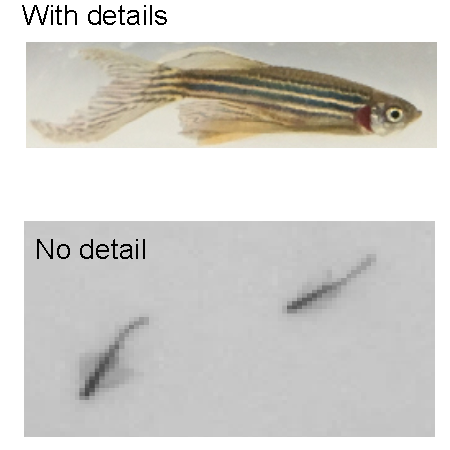
\includegraphics[width=\marginparwidth]{fish-detail}
\captionof{figure}[The morphological detail of a fish]{
	Top: a picture of zebrafish with various details. Bottom: a picture of two zebrafish with no detail.
}
\label{fig:fish-detail}
}

In the methods section, the ideas needed to carry out no-detail tracking will be discussed. The result of 2D swimming experiment, analysed by our method, will be presented in the results section. The 2D coordinates of zebrafish revealed two essential features. Firstly the spatial distribution of the fish was inhomogeneous. The effective pairwise interaction of the fish seemed attractive, and the attraction appear to decrease with the number of individuals in a group.

\section{Methods}

%Observing the fish in the lab includes the construction of the hardware, and the development of the software. Both of them will be covered in the method section. The 2D tracking code will be reused in chapter~\ref{chapter:fish_3d} as the basis for 3D tracking. 

\subsection{Fish and Apprautus}
\label{section:apprautus_2d}

The adult zebrafish, whose age is over one year old, were used to carry out the experiment. Most experiments in this section was carried out in the fish facility in Bristol, while some experiments were performed in room G59 in the HH Physics Laboratory in Bristol. The fish were fed three times a day, with natural day to night circles. The fish were hosted in their living tank before the experiments, with a density of 5 fish per litre of water. The water was filtered constantly, with a pH value close to 7 and the temperature close or above 25 °C.

Before each experiment, the fish were transferred from their living tank to the experimental environment, which will be referred to as the {\ot}. During the transfer, the fish were placed inside a temporary container, and then released into the {\ot}.
To make the fish stay in a quasi-2D environment, a flat plate was placed in a bowl-shaped tank, creating a shallow water environment (Fig.~\ref{fig:fish_apprautus_2d}). The shape of the bowl is especially chosen for a 3D tracking task, which will be introduced in chapter \ref{chapter:fish_3d}.



\begin{SCfigure}[][!ht]
  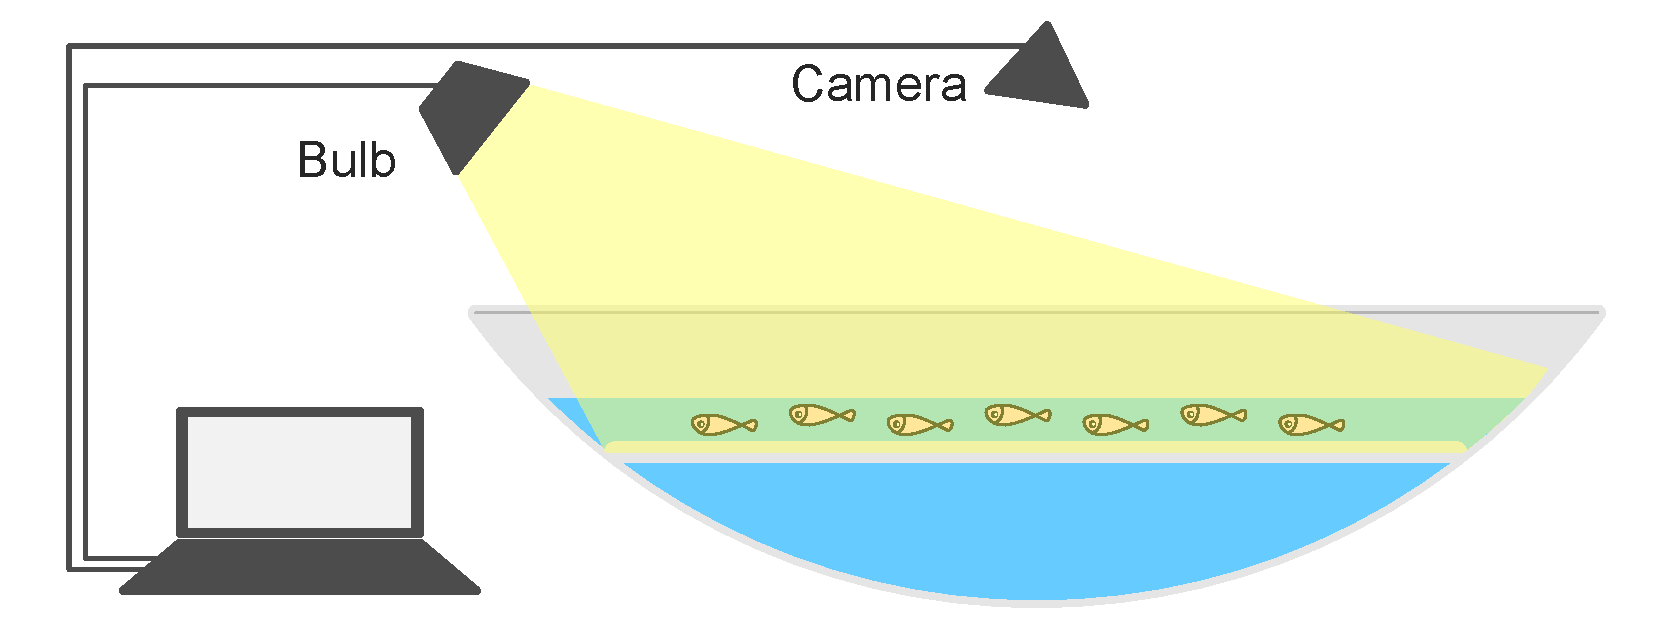
\includegraphics[width=\linewidth]{apprautus-2d}
  \caption[Two dimensional fish tracking apprautus]{\label{fig:fish_apprautus_2d}
  The apprautus to track the movement fish in a quasi-2D environment. The camera is placed above the fish to capture the top view. A computer controls the recording process as well as the illumination.
  }
\end{SCfigure}


\subsection{Metric Rectification}
\label{section:metric_rectify}


To record the video of the fish, a camera (Basler AC2040um) was fixed on top of the tank, as illustrated in Fig.~\ref{fig:fish_apprautus_2d}. The image size produced by our camera is 2056 pixels $\times$ 1540 pixels, at a frequency of 15 frames per second.
We mounted a 6 mm fixed focal length lens (C Series, Edmund Optics) on the camera, which yields a wide view, allowing us to place the camera closer to the fish group. The typical distance between the camera and the fish group is around 2 meters. With such setup, the fish (body length $\sim$ 30 mm) appear as black rods in the videos, as shown in Fig.~\ref{fig:metric-rectify}.


The image and videos obtained from the camera have three limitations, preventing it from being an accurate measurement tool.
The first issue is the distortion of images caused by the camera lens.
In addition, the cameras should be orientated exactly perpendicular to the water surface, so that the captured images were from the top view. Such accurate orientation is difficult to achieve without especially designed camera holders.
Finally, we also need to convert the unit of the image (pixels) to real life units (e.g. meters).
It is worth mentioning that these issues were more or less ignored in conventional 2D animal tracking tasks \cite{panadeiro2021}, and the present method is novel in the context of animal tracking.\marginfootnote{
Addressing these issues is ``less novel'' in the computer vision community focusing on the 3D reconstruction. It is impossible to retrieve 3D information correctly without understanding all the details about computers and photos.
}

To solve the problems, we need to \emph{calibrate} the camera, so that we know the distortion of the camera lens, the orientation of the camera, as well as the scale of objects in the images. To carry out the calibration, a chessboard (the calibration board) was placed on the surface of the water. And the image of the calibration board will offer enough information to tackle the aforementioned issues. 

The distortion can be recovered with standard camera calibration methods\marginfootnote{
The functions from the ``opencv'' library were used for the calibrations.
}
from the computer vision community \cite{ma2005, hartley2003}. The distortion is described with the following model,

$$
\begin{aligned}
x_{\text {distorted }} &= x\left(1+k_{1} r^{2}+k_{2} r^{4}+k_{3} r^{6}\right) \\
y_{\text {distorted }} &= y\left(1+k_{1} r^{2}+k_{2} r^{4}+k_{3} r^{6}\right)
\end{aligned}
$$

\noindent where $r$ is the radius of the pixels in the image with respect to the optical centre. And $k_i$ values are the distortion coefficients, which will be used to recover the undistorted image.


The imperfect orientation can be fixed by the knowledge of the camera as well. Briefly, the same 2D plane in the 3D space, will form different projections with different cameras. 
These different 2D projections are related to each other by a projective transformation.
Likewise, the same 2D plane for the fish in the imperfectly orientated camera is also related to its counterpart from a perfectly orientated camera.
Such a relation is termed as \emph{homography}
%\marginfootnote{Further description of the projective transformation, as well as the calculation of $\mathbf{H}$ is included in the appendix~\ref{chapter:multi_view}.}
, and can be represented by a matrix
$\mathbf{H} \in \mathbb{R}^{3 \times 3}$. This matrix can be calculated easily with the knowledge of the camera, following the method from \citeauthor{hartley2003} \cite{hartley2003}.
The homography allows us to transform the image from the imperfectly orientated camera, to a virtual image captured from a perfectly orientated camera. The transformed image is called the \emph{rectified image}.
From the rectified image, the scale can be recovered easily as we know the physical size of the calibration board. We call the rectified image with a known scale the \emph{metrically rectified image}.


Figure~\ref{fig:metric-rectify} shows an example of the metric rectification. Comparing the outline of boundary with/without distortion removed, it is clear that the raw image from the camera were distorted by the lens. The camera in the experiment were not perfectly perpendicular to the water surface, therefore the outline of the tank boundary appears to be an ellipse, because of the perspective transformation (\gls{homo}). The ellipse were reverted back to a circle (right subfigure, Fig.~\ref{fig:metric-rectify}) after the rectification process.

\begin{SCfigure}
  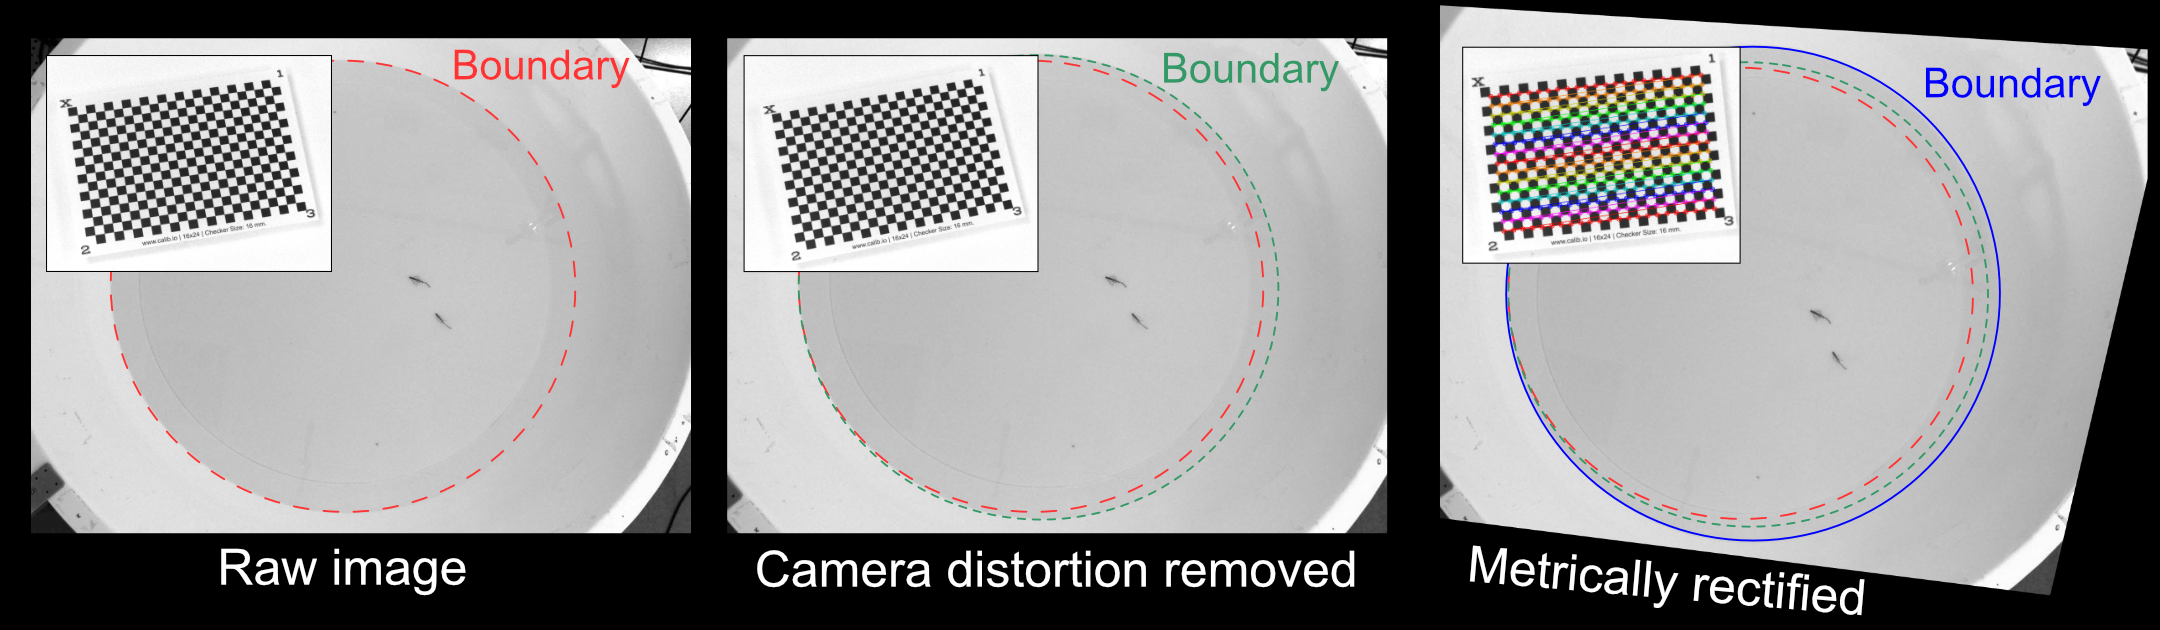
\includegraphics[width=\linewidth]{image-calib-2d.png}
  \caption[Metrical rectification of an image.]{
  	The process of metrical rectification. Left: the original image. Middle: the image where camera distortion being removed. Right: the metrically rectified image. The circular outline of the 2D boundary were outlined and overlaid, to stress the change of the image in different steps. The inserts in the figures correspond to the calibration pattern in each process.
  }
  \label{fig:metric-rectify}
\end{SCfigure}

Notably, the image rectification only ``works'' for the plane, where the calibration chessboard lies. For the fish data, the rectification is only accurate for the fish exactly swimming on the water-air interface. In other works, there will be tiny errors for the fish locations, when they swim inside the water. Such inaccuracy is fundamental for 2D fish tracking, since the fish is swimming a 3D space. To eliminate such error, we can carry out real 3D measurements, which will be introduced in chapter~\ref{chapter:fish_3d}.


\subsection{Image Processing}
\label{section:image_process}


The metrically rectified images of the fish contain the information about their behaviour.
To get useful information out of the image, we still need to perform image processing, to extract the coordinates of the fish from the images.

In a normal image, the fish appear as a dark spot (see Fig.~\ref{fig:metric-rectify} and Fig.~\ref{fig:2d_process} for instances).
Ideally, we want to work with images containing a collection of delta functions (see middle subplot of Fig.~\ref{fig:locate-cnn} for instance), where the pixel intensities in the centres of each individual fish is maximised, and the pixel intensities are zero everywhere else. Extracting the coordinates of fish from such image, will therefore be a trivial task, as we only need to find the pixels with non-zero values. Even though it is possible to construct such transformation directly with machine learning based approaches \cite{newby2018}, it is still not an easy task, without large amount of human labelled training data. Therefore, we restrict our goal for the image processing process to be the removal of the static background. As a result, the processed image should only contain the fish.

Traditional image processing methods, such as thresholding, blurring, and morphological operations, were used in this project to perform the background removal task.
As a result, we get a \emph{foreground video} where each fish has high pixel intensity values, and the background intensity values are zero. Figure \ref{fig:2d_process} illustrates the result of the transformation. One frame of the recorded video was shown in the left subfigure, while the same frame from the foreground video was shown in the right subfigure.


\begin{SCfigure}
  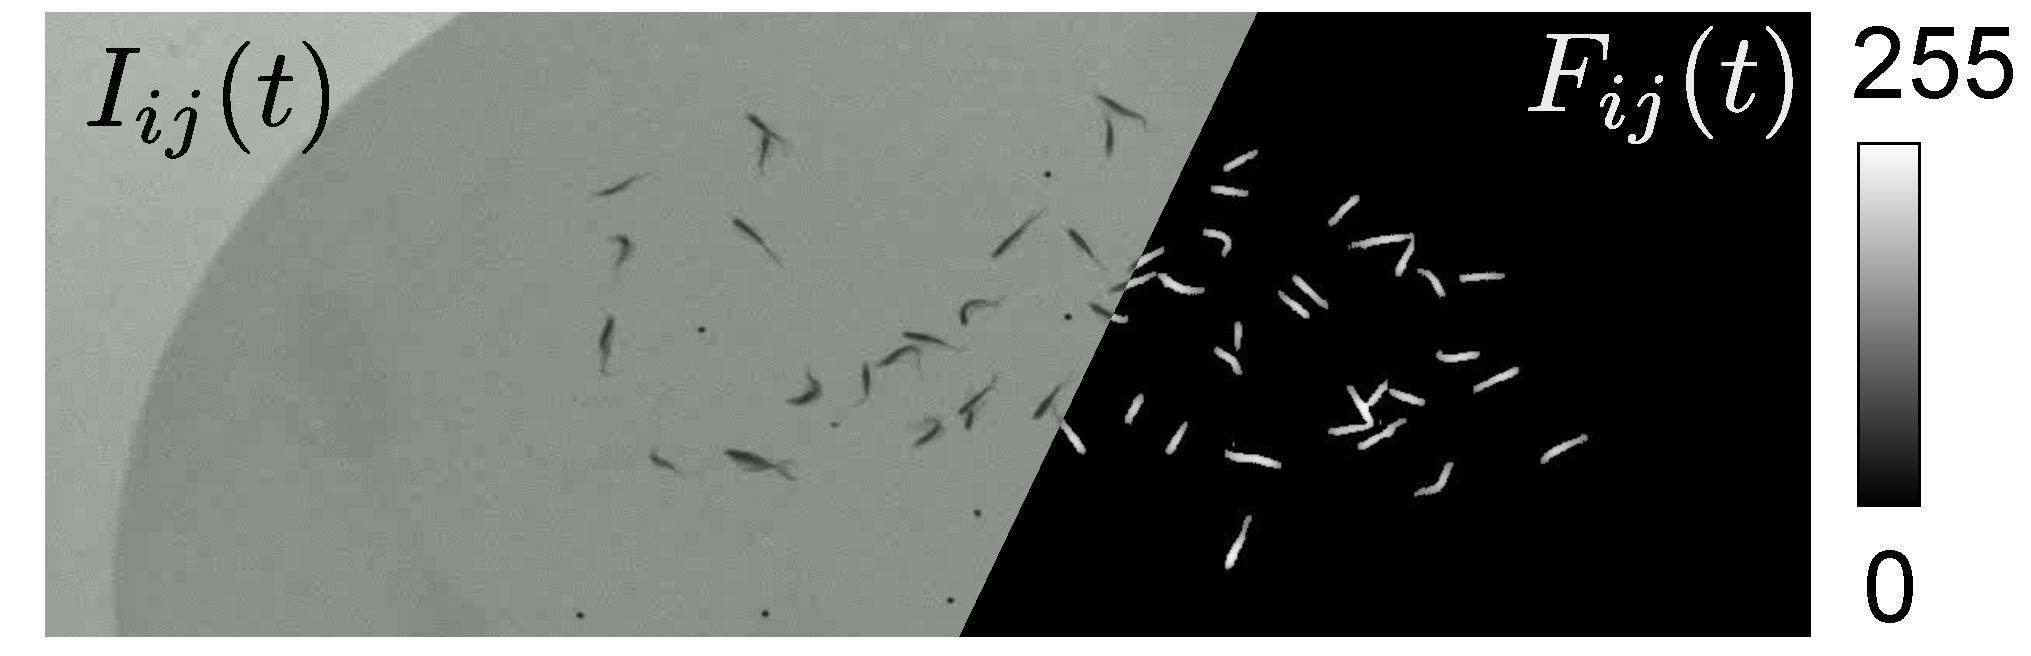
\includegraphics[width=\linewidth]{image-process}
  \caption[Two dimensional image processing.]{
  The screenshot of the video at time point $t$, and its corresponding foreground image.
  }
  \label{fig:2d_process}
\end{SCfigure}


The foreground videos of the fish are obtained after two  steps, the removal of the background and the removal of the noises. 
The background is defined as the temporal average of the image, since the fish are constantly moving while rest of the scene is static. In order to tackle the varying illumination conditions,
we can take a running average of a time--window, instead of calculating the overall average. The pixel intensity of the background (\gls{bijt}) at time \gls{t}, of pixel $(i, j)$, can be written as

\begin{equation}
	B_{ij}(t) = \frac{1}{T_w} \sum_{\tau=t}^{t+T}{I_{ij}(\tau)}
\label{eqBG}
\end{equation}

\noindent where \gls{iijt} is the pixel intensity of the video at time \gls{t} in position $(i, j)$, and $T_w$ is the duration of the window, usually taken as 40 seconds. The difference between the background video and original video yields a foreground video (\gls{fijt}), written as

\begin{equation}
	F_{ij}(t) = B_{ij}(t) - I_{ij}
\label{eqFG}
\end{equation}

\noindent and the order of the subtraction ensures the fish, originally appear darker in the video, to be represented by brighter pixels in the foreground video. The subtraction result can be very noisy. To remove the noise, the gaussian filter was applied to the foreground image. Then, the combination of the Ōtsu threshold and local Gaussian threshold was applied to the image, to separate the pixels belonging to the fish and other pixels.
The Ōtsu threshold is a single value that split the image into two groups, where the inter--group variance was minimised. The local Gaussian threshold, on the other hand, gives a collection of different values for different pixels, featuring the locally bright pixels as foreground. Finally, the morphological operation ``binary opening'' was applied to the image, to remove any possible remaining noise. The results shown in Fig.~\ref{fig:2d_process} was obtained with this method.

Our method requires 3 parameters, including the standard deviation (\gls{sigblur}) of the  Gaussian kernel of the blurring process, the length scale for the local threshold (\gls{llt}), and the length scale of the binary open operation (\gls{lbo}). In the different experiments, the images were similar, therefore the same set of parameters ($\sigma_\mathrm{blur}=2, l_\mathrm{local}=3, l_\mathrm{open}=3$) was applied, and works well for most videos.



\subsection{Extracting Features from the Image}
\label{section:feature}



From the processed video, we need to extract the features\marginfootnote{
We explained the term ``features'' by the end of the section.
} in each frame that correspond to the fish. In order to tackle the problem, we employed a method that not only captured the positions, but also the information of the fish orientations and body shapes. The basic idea is to calculate the cross--correlation between the image ($F_{ij}$) and a templated fish shape (\gls{tij}), as the local maxima in the result would indicate the presence of a fish, because cross--correlation is a measure of similarity between signals.


For a fixed 2D fish template (\gls{tij}), we can rotate it so that it contains $o$ different orientations. Calculating the cross-correlation of all the rotated templates, we can effectively get $o$ different results, and they can be concatenated into a 3D tensor, written as \gls{cijo}. One can think of the tensor $C_{ijo}$ as a 3D volumetric image. A local maximum in $C_{ijo}$, with coordinate $(i_m, j_m, o_m)$, indicates the presence of a fish at location $(i_m, j_m)$, with orientation $o_m$.


In addition, we are free to choose different templates for the fish shape, to capture the different postures. The choice for the template will be discussed in section~\ref{section:template}. If $s$ different shapes were selected as templates, all of which were rotated into $o$ different orientations, then there will be $s \times o$ different templates. The cross-correlation of these templates with the image would yield a 4D tensor that can be shaped into \gls{cijos}, noted as the \emph{feature tensor}. A local maximum of the feature tensor, with coordinate $(i_m, j_m, o_m, s_m)$, represents a fish located at $(i_m, j_m)$, whose shape is like the $s_m$th template, with orientation $o_m$. All the local maxima, {$\{(i_m^i, j_m^i, o_m^i, s_m^i)\}$}, captured the locations, orientations and shapes of all the fish in the image.

\begin{SCfigure}
  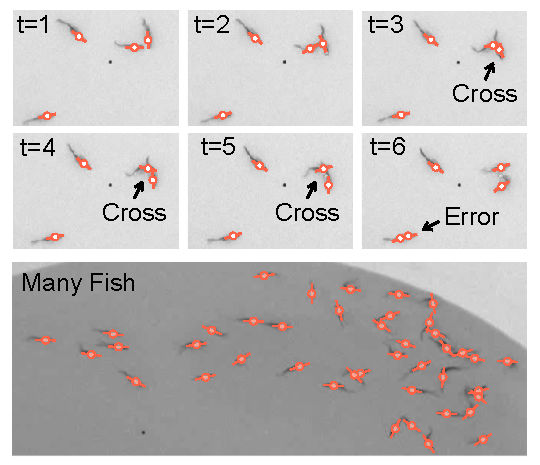
\includegraphics[width=\linewidth,outer]{features}
  \caption[The correct label of overlapping fish.]{
  The locations and orientations, $\{(i_m, j_m, o_m)\}$, of different fish. The locations are rendered as circles, while the orientations were rendered as short line segments.
  The features were calculated from the feature tensor ($C_{ijo}$).
  Top: the movement of 4 fish in 6 successive frames labelled with the detected features. An error where one fish was mistakenly labelled as two fish happened in the 6th frame.
  Bottom: the movement of many fish labelled with the detected features.
  }
  \label{fig:fish_features}
\end{SCfigure}

In summary, the cross--correlation between the image and the many templates yields a 4D feature tensor, whose local maxima give us the locations, orientations, and shapes of different fish. This approach is especially helpful for the dense system, where the fish constantly overlap with each other. In such dense scenario, the overlapping fish will be separated into different regions in the shape--rotation dimension in the feature tensor. For example, the overlapped fish pair in Fig.~\ref{fig:fish_features} was correctly labelled, by calculating the local maxima in the 4D tensor.


There is a fundamental flaw of our algorithm, where a big fish might be mistakenly labelled as two small fish. One example of such error was presented in Fig~\ref{fig:fish_features} (top row, t=6).
This is partially due to the loss of morphological details of the fish, as the cameras were placed relatively far from the fish, in order to capture larger groups.
Without the details, it can also be hard for a human being to tell, whether a dark blob is a big fish or it belongs to two smaller fish. Realistically, some of the errors produced by our algorithm can be easily distinguished by human beings. Some post processing methods of the features, based on the geometry of the fish, might be useful to further refine our algorithm. The ultimate goal is to make the feature detection algorithm being compatible with human observations.


\begin{tcolorbox}[
title={Why are features called features, not positions?},
enlarge bottom by=0.5em,
enlarge top by=0.5em,
]
In the computer vision community, people call the locations of objects ``features''. This term is rooted in the 3D reconstruction problem, which will be discussed in the chapter~\ref{chapter:fish_3d}. Briefly, the 3D information can not be recovered from the background, like a purely white wall. Instead, some ``features'' with intensity gradients are required \cite{ma2005}. Alternative names would be ``positions'' or ``locations''. However, we are interested in a ``feature'' of the photo, rather than a (physical) location of a fish.
\end{tcolorbox}

\subsection{Finding Templates for the Features}
\label{section:template}


To calculate the feature tensor $C_{ijos}$, it is important to use suitable templates for the fish. The templates should represent characteristic fish shapes.
%The unsupervised machine learning methods from the computer vision community are suitable in this situation .
The following operations were carried out to find suitable templates.

\begin{enumerate}
	\item Segment the individual fish and align the segmented images.
	\item Project all the segmented images to a space with reduced dimension.
	\item Find clusters for the data points in the reduced space, and the average of each cluster to be the template.
\end{enumerate}

The individual fish, defined as connected bright pixels, were segmented from the foreground video ($F_{ij}(t)$).
The orientation of the segmented fish were determined by the principle component analysis (\gls{PCA}) \cite{goodfellow2016}. 
These segmentations were then reoriented, so that its first principle axis align with the $x$ axis. The reoriented individual fish were then zero-padded to have the same shape, noted as $\mathbf{S} \in \mathbb{R}^{s \times s}$ where $s$ is the size of the padded images.
Examples of the segmented and aligned images are illustrated in Fig.~\ref{fig:fish_segment}. These images were collected over 1000 different frames, in a video of 4 swimming fish. A total of 3070 individual shapes were collected.

\begin{SCfigure}
  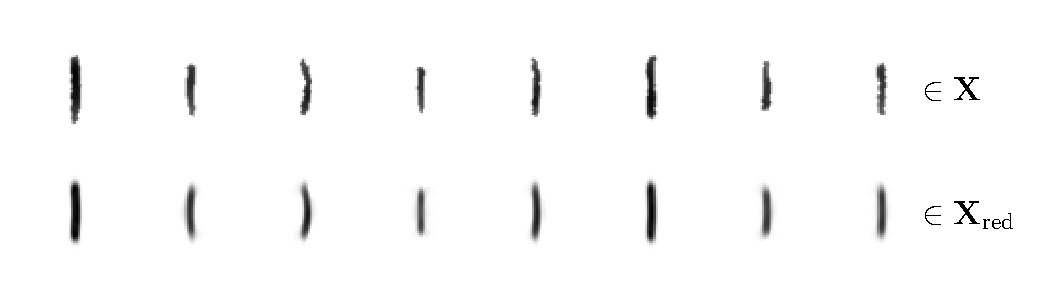
\includegraphics[width=\linewidth]{shapes}
  \caption[Examples of segmented individual fish]{
  Top: the selected individual fish segmented from the images taken by the camera.
  Bottom: the fish shapes reconstructed from a low dimensional feature space $\mathbf{X}_\mathrm{red}$.
  }
  \label{fig:fish_segment}
\end{SCfigure}

The collection of segmented fish is a very large dataset.
For example, if we use a small image of size $50 \times 50$ pixels, to stored each fish, then each fish corresponds to a point in a 2500 dimensional space.
The dimension of such images can be drastically reduced by PCA \cite{solem2012book, geron2019}. Operationally, all of the $m$ images of individual fish were flattened
($\mathbb{R}^{s \times s} \rightarrow \mathbb{R}^{s^2}$),
and concatenated into a matrix ($\mathbf{X} \in \mathbb{R}^{m \times s^2}$).% For the dataset presented in Fig.~\ref{fig:fish_segment}, $m=3070$.
The singular value decomposition (\gls{SVD}) is then performed on the dataset $\mathbf{X}$, following

$$
\mathbf{X} = \mathbf{U} \Sigma \mathbf{V}^T,
$$

\noindent where the matrices $\mathbf{U}$ and $\mathbf{V}$ contains all the left and right singular vectors, and the matrix $\Sigma$ contains all the singular values. The images ($\mathbf{X}$) were then project on the first $k$ axes ordered by their corresponding singular values. Effectively, the dimension of the matrix $\mathbf{X}$ were reduced from $m \times s^2$ to $m \times k$, forming a new matrix $\mathbf{X}_\text{red} \in \mathbb{R}^{m \times k}$. Each row in $\mathbf{X}_\text{red}$ described one fish.



Figure~\ref{fig:fish_pca} shows the average fish shape as well as the projection of all the segmented fish ($\mathbf{X}$) on the first two principle axes. The first principle axis (the $x$ axis of Fig.~\ref{fig:fish_pca}) roughly captured the scale of the fish, and the second principle axis (the $y$ axis of Fig.~\ref{fig:fish_pca}) captures the information about the bending of the fish. 
The overall distribution of those projected data can be understood by the fact that the same fish can have different distances and orientations, relative to the camera, so that their shapes will appear different.
The distribution of Fig.~\ref{fig:fish_pca} is symmetric in the $y$ direction, which indicates the absence of chirality for the bending of fish. That is to say, the fish do not prefer bending to the left, or the right.

With all the segmented fish being projected to low dimensional space, we can use the \emph{k-means cluster} algorithm to find representative cliques of the fish shapes.
Briefly, different data points (different fish images in Fig.~\ref{fig:fish_segment}) will be assigned to different clusters. And the variance of points in the same cluster will be minimised, while the variance of points from different clusters will be maximised.

Each cluster corresponds to similar fish images with similar shapes. The average shape of different clusters were used as the template. The different scatters in Fig.~\ref{fig:fish_pca} shows the different clusters, and their corresponding average shapers were inserted. Here, the images ($\mathbf{X}$) were projected to a 2 dimensional space ($k = 2, \mathbf{X}_\text{red} \in \mathbb{R}^{3070 \times 2}$). And the overall 3070 points were separated into 7 different clusters. And the average shape of different clusters (the inserted subplots in Fig.~\ref{fig:fish_pca}) can be used as the templates to calculate the 4D tensor for tracking.



\begin{SCfigure}
  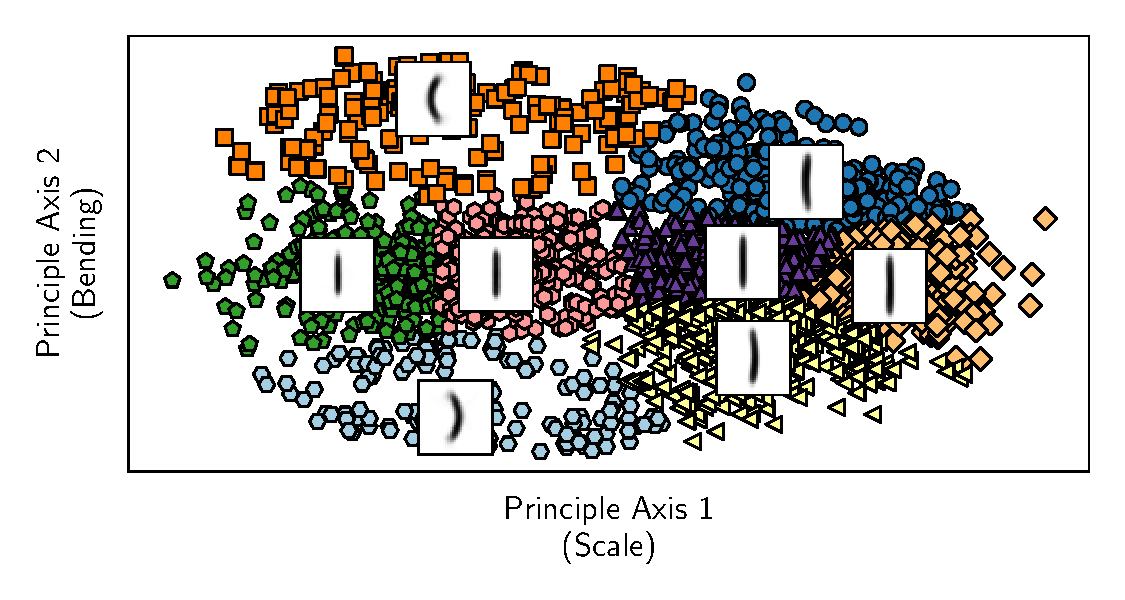
\includegraphics[width=\linewidth]{fish-pca-proj}
  \caption[PCA analysis of the fish shape]{
  A collection of 2170 different fish shapes, projected onto the first two principle component axes. The data points were clustered using the K-means algorithm, into six different clusters, indicated by different marker styles. The average shape of each cluster were plotted in the inserted axes.
  }
  \label{fig:fish_pca}
\end{SCfigure}


The number of clusters and the dimension of the reduced space ($k$) are free parameters, whose optimal values were hard to determine. Practically, I always set $k=5$, and separate the points into 8 different clusters, which yields good\marginfootnote{
If the 2D features are not good, the corresponding 3D reconstruction (chapter~\ref{chapter:fish_3d}) will fail.
} results for 2D tracking. The dimensional reduction method (PCA) and the clustering algorithm (K-means) can be changed to other tools with similar effects. For instance, it is possible to use non-linear dimensional reduction method such as isomap, and a gaussian mixture model to obtain different clusters.

The mapping from the image to the large 4D tensor, $I_{ij} \rightarrow C_{ijos}$ requires a large amount of calculation. The feature tensor is normally sparse, since only a few pixels in the image contain the centre of the fish. The calculation can be faster if such sparsity were to be exploited.
Practically, we can only calculate ``promising'' pixels, where fish is likely to appear. These pixels correspond to the local intensity maxima in the foreground image $F_{ij}$. Such reduction of calculation improved the calculation speed significantly.


\subsection{Convolutional Neural Network}
\label{section:cnn}



There are two steps in the image processing that can be improved in the image processing pipeline. The first one is the removal of background. In my current method, I calculated a rolling average of the entire video. The window size of the averaging operation is set by the user, which is very difficult to optimise because the video processing typically takes hours to finish. Practically, a rule-of-thumb number (600 frames) was applied. However, the fish in the video are very distinct from their background, and it is an easy task for people to spot the fish in a static image. This suggests a static image contains enough information to distinguish the foreground (fish) and background (tank). 

The convolutional neural network (\gls{CNN}) is very suitable for carrying out both tasks at the same time, with far better efficiency. The overall data process introduced from section~\ref{section:image_process} to section~\ref{section:template}, is essentially a transformation from the image ($I_{ij}$) to a tensor ($C_{ijos}$). In addition, the information about the kernel is unnecessary\marginfootnote{
The shapes might be informative for people studying the postures of the swimming fish. But we will ignore the shapes in this thesis as we are interested in the \emph{collective motion} of the fish.
} in most cases, as we often only care about the orientation and location of the fish, rather than its shape. Hence, we need a model with the capacity to carryout the following transformations depending on our desired results:

$$
\begin{aligned}
I_{ij} &\rightarrow C_{ijos} 
&\textrm{location, orientation, and shape} \\[1ex]
I_{ij} &\rightarrow C_{ijo}\;(= \max_{s}{C_{ijos}})
&\textrm{location, and orientation} \\
I_{ij} &\rightarrow C_{ij}\;(= \max_{o}{C_{ijo}})
& \textrm{location} \\
\end{aligned}
$$

\noindent And we can generate a big dataset containing images ($I_{ij}$) and their corresponding feature tensors ($C_{ijos}$), and make a CNN to learn the underlying rules for the transformation ($I_{ij} \rightarrow C_{ijos}$). If we need less information from the result, the targeted $C$ can be contracted, by taking the maximum value along the dimension of the unnecessary information.

\begin{SCfigure}
  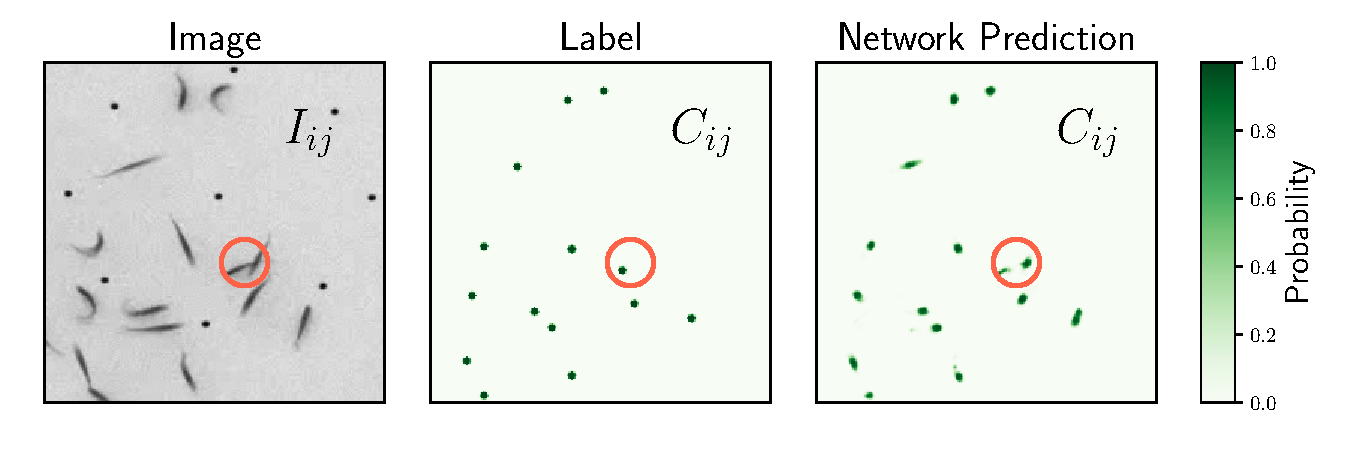
\includegraphics[width=\linewidth]{locate-cnn}
  \caption[The feature tensor calculated with convolutional neural network]{
	The tracking result of a convolutional neural network (CNN).
	Left: the image ($I_{ij}$) from which the fish will be detected.
	Middle: the feature tensor (\gls{cij}) for all the pixels generated by a conventional 2D tracking algorithm. This data is used as training data for the neural network. The value of a pixel in the tensor represents the probability that a fish centre being located inside this pixel. 
	Right: the feature tensor ($C_{ij}$) for all the pixels predicted by the CNN model. The network prediction should be close to the label after the network being trained.
  }
  \label{fig:locate-cnn}
\end{SCfigure}


As a proof of concept, a CNN model was built to carry out the transformation of $I_{ij} \rightarrow C_{ij}$. The training data for the network was generated from the existing tracking result $C_{ijos}$.
The model was built with popular framework tensorflow \cite{tensorflow2015}, and trained on the Colab online platform provided by Google \cite{carneiro2018}.
Figure~\ref{fig:locate-cnn} shows the output of a trained network. The network does not generate the exact same picture of the label, but their results were similar. Notably, the network even fixed an error of the original feature detection algorithm. This error is highlighted in Fig.~\ref{fig:locate-cnn}. 

However, due to the limited time for this project, the final CNN model did not improve the calculation accuracy nor the processing speed significantly. Nevertheless, it is achievable to having the calculations to be optimised that the tracking can be performed in real time, since the prediction of $C_{ij}$ on a GPU is very fast, reaching a speed of $\sim 50$ frames per second. The current speed-limiting step is the calculation of local maxima in $C_{ij}$ with CPU. This calculation can be accelerated by either exploiting the sparsity of $C_{ij}$, where local maxima detection can be converted to an overlapping removing problem (see section \ref{section:overlap}). Alternatively, it might also be helpful to carry out the calculation on GPU.


\section{Results}

In this section, the spatial distribution of zebrafish will be presented. For all the data shown below, the fish that were not swimming was excluded from the calculation. The swimming fish was defined as the fish whose swimming speed is larger than 60 mm/s. This specific value was chosen, based on the fact that the average speed of zebrafish is around 120 mm/s.

\subsection{A Single Fish}
\label{section:fish_1_2d}

\marginpar{
\centering
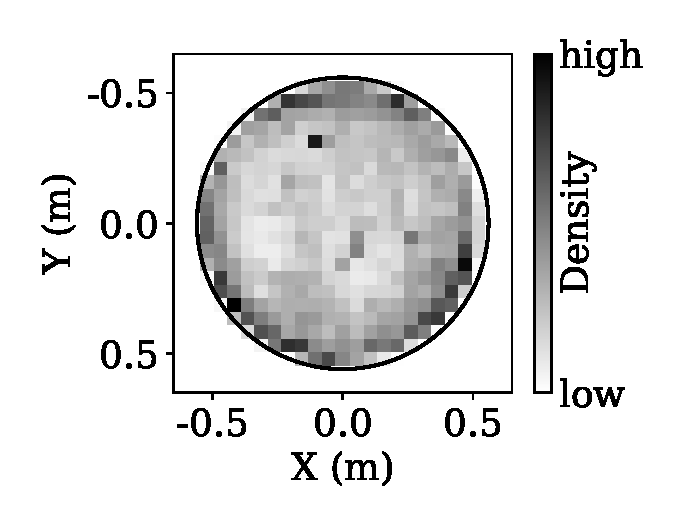
\includegraphics[width=\marginparwidth]{dist-1-fish}
\captionof{figure}[The 2D spatial distribution of 1 adult zebrafish]{
The spatial distribution of two adult zebrafish in a quasi 2D environment, present the joint distribution of the $x$ coordinates and $y$ coordinates of the fish positions, with the shape of the boundary being highlighted.
}
\label{fig:density_2d_fish_1}
}


Figure~\ref{fig:density_2d_fish_1} shows the spatial distribution of one adult wildtype zebrafish. We can see from the figure that the fish have a slightly higher tendency to stay near the boundary. The apparent attraction between the fish and the boundary can have two reasons. Firstly, the fish may biologically prefer to be near the boundary. The systematic preference for the wall of the tank was documented for zebrafish previously \cite{seguret2016}. 

In addition, the preference to the wall of the fish could emerge as a physical consequence, if we think of fish as self-propelling particles \cite{lee2013, maggi2015, bechinger2016}, as justified in section~\ref{section:active-matter}. To understand this physical origin, it is helpful to to imagine a fish who changes its orientation randomly. Without the boundary, the fish would move constantly, regardless of its orientation. On the other hand, if the fish were swimming against the wall, they have to wait until the orientation changes, to leave the wall and continue swimming. The extra waiting period near the wall would contribute to the spatial distribution.



\subsection{Two Fish}
\label{section:fish_2_2d}

The movement of 2 adult zebrafish was recorded. The data was taken over 5 experiments, and each experiment lasted one hour.
The spatial distribution of 2 fish were shown in Fig.~\ref{fig:density_2d_fish_2} (left). It is clear that the fish were not uniformly distributed in the tank, which might also related to the environmental factor \cite{makris2006, rosemberg2011, shelton2020}.

\begin{SCfigure}[][!ht]
  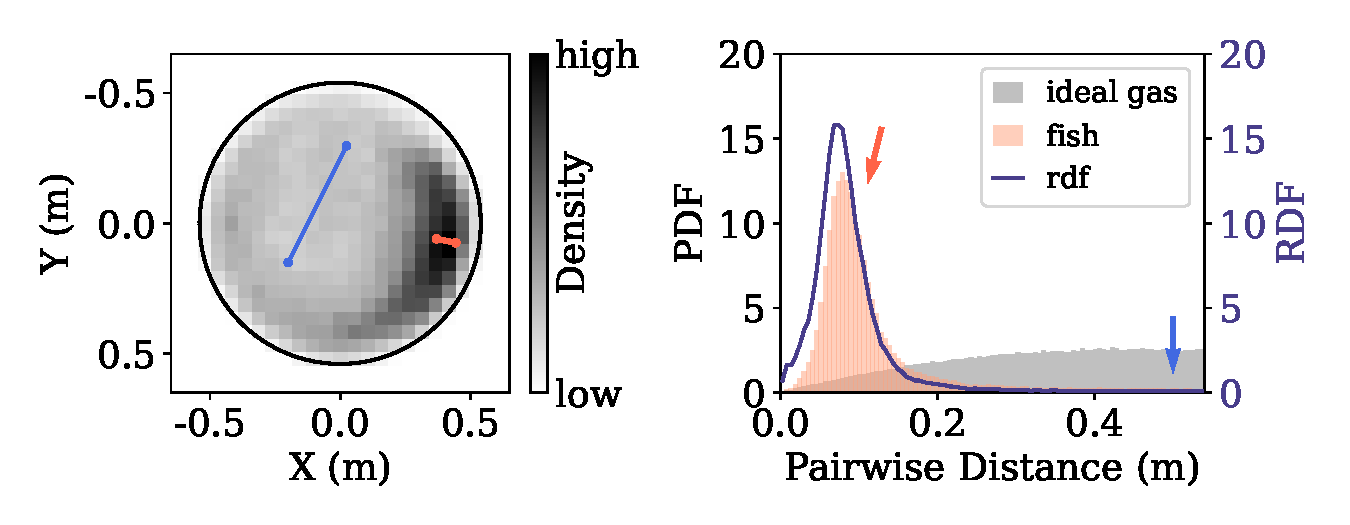
\includegraphics[width=\linewidth]{dist-2-fish}
  \caption[The 2D spatial distribution of two fish]{The spatial distribution of two adult zebrafish in a quasi 2D environment. Left: the joint distribution of the $X$ coordinates and $Y$ coordinates of the fish positions, with the shape of the boundary being highlighted. Right: the probability density function (PDF) for the distance between two fish. The PDF for the distance of 2 ideal gas particles, uniformly distributed in the tank, were also plotted. The ratio of the two \gls{PDF}s were taken as the radial distribution function (RDF).}
  \label{fig:density_2d_fish_2}
\end{SCfigure}

The pairwise distance of the 2 fish offered us the way the characterise their cohesion. If the fish were attracted to each other, they would stay close, and vice versa. The distribution of the pairwise distances, shown as the probability density function (PDF), were plotted in the Fig.~\ref{fig:density_2d_fish_2} (right). There is a peak in the distribution, and it seems to be dominated by the inhomogeneous distribution of the fish, as the length scale corresponding to the peak matches the size of the high density blob. Such a length scale was highlighted in Fig.~\ref{fig:density_2d_fish_2} (left).




It is useful to compare the distribution of the pairwise distance of the fish, with the distribution from the ideal gas. Here ideal gas means random points uniformly distributed in the circular tank outlined in Fig.~\ref{fig:density_2d_fish_2}. The distribution of the ideal gas were presented in Fig.~\ref{fig:density_2d_fish_2} (right). The probability of finding particles at large distances, like 0.5 meter, is higher for the ideal gas particles comparing with fish. This is also likely due to the inhomogeneous distribution of the fish, as such length scale corresponds to a big ``void'' in Fig.~\ref{fig:density_2d_fish_2}.

Inspired by liquid state theory, we define the ratio between the PDF of the fish and that of the ideal gas as the radial distribution function (\gls{RDF}), which is also known as the \gls{gr}, as introduced in section~\ref{section:intro-analysis}.
For a dilute fluid at equilibrium, the shape of its RDF can be used to calculate the pairwise interaction potential. The mapping between pairwise potential and the $g(r)$ is invalid for the fish, because the individuals were constantly spending their biological energy to swim, driving the system out of equilibrium.
Nevertheless, $g(r)$ is still a useful tool to characterise the cohesiveness of the fish group. The RDF of 2 fish are plotted in Fig.~\ref{fig:density_2d_fish_2}, and it presents a peak at very short separation. The hight of the peak ($\sim 15$) offered a measure of the attraction amongst the fish, and more detailed analysis will be provided in chapter~\ref{chapter:fish_analysis}.


\subsection{Three Fish}
\label{section:fish_3_2d}


\begin{SCfigure}
  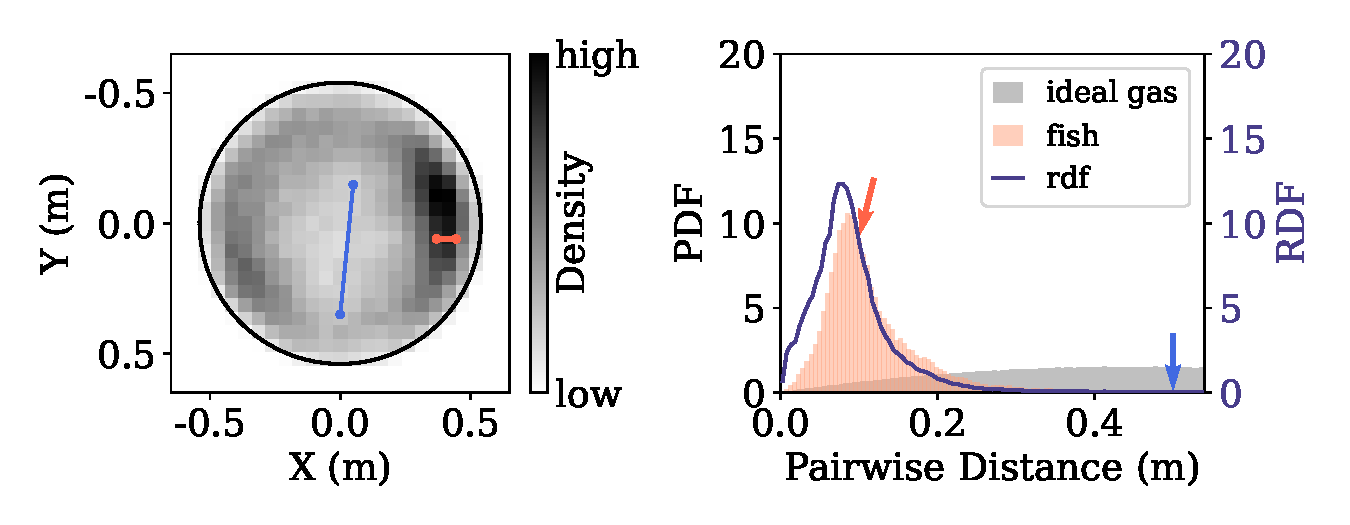
\includegraphics[width=\linewidth]{dist-3-fish}
  \caption[The 2D spatial distribution of three fish]{The spatial distribution of three adult zebrafish in a quasi 2D environment. Left: the joint distribution of the $X$ coordinates and $Y$ coordinates of the fish positions, with the shape of the boundary being highlighted. Right: the probability density function (PDF) for the distance between two fish. The PDF for the distance of 3 ideal gas, uniformly distributed in the tank, were also plotted. The ratio of the two PDFs were taken as the radial distribution function (RDF).}
  \label{fig:density_2d_fish_3}
\end{SCfigure}


The behaviour of 3 adult zebrafish is very similar to that from 2 fish. The density distribution and the distribution of pairwise distances of 3 zebrafish were shown in Fig.~\ref{fig:density_2d_fish_3}. Like the situations in the one fish and 2 fish system, the distribution is not uniform. And the fish also present a typical peak in the pairwise distance, whose location (~0.08 m) corresponds to the size of the high density blob of the inhomogeneous distribution.


Comparing the PDF of the pairwise distance of the fish, with that from 3 ideal gas, the fish also presents the typical void like the 2 fish scenario. The RDF for 3 fish, shown in Fig.~\ref{fig:density_2d_fish_3} (right) is very similar to that of 2 fish. The height value of the peak for 3 fish is close to 12, being slightly smaller than that from 2 fish experiments. One possible explanation for such reduced attraction, is the reduced danger perceived by the fish, when they were in a large group \cite{spence2007}.
%\marginfootnote{This reference is not very convincing.}.
As the fish will form a denser group when they perceived danger \cite{perez-escudero2017}.
 As well be presented later, the reduced cohesion with increased group number is a general observation.



\subsection{Many Fish}
\label{section:fish_50_2d}

The distribution of 50 fish was significantly different from the 1/2/3 fish results, as presented in Fig.~\ref{fig:density_2d_fish_50}.
Comparing with the 1/2/3 fish experimental results, the density distribution of 50 fish were more homogeneous, shown in the left subfigure in Fig.~\ref{fig:density_2d_fish_50}. However, it is still not uniform. The homogenised picture for 50 fish might be related to the fact, that the fish-fish interaction dominates the behaviour for 50 fish, while fish-environment interaction dominates the behaviour of 1/2/3 fish. The same trend was also observed in a 3D swimming experiment, which will be discussed in section~\ref{section:fish_many_3d}.

In addition, the PDF of the pairwise distance for 50 fish were much broader comparing with its 2 or 3 fish counterpart. Nevertheless, we still see the same trend, where the fish were cohesive in short length scales, and presented ``void'' at larger separation distances. Such feature is also likely due to the inhomogeneity of the density distribution. However, the difference of the PDFs for the 50 fish and 50 ideal gas particles was less significant. As a result, the RDF of the 50 fish contains only a broad peak, whose height value ($\sim$ 3) is significantly smaller the height value of the RDF for 2 or 3 fish. This suggested a smaller effective attraction between the fish when they were in a large group. Our observation, the reduction of peak height in the RDF, is consistent with previous study \cite{romenskyy2017}.

\begin{SCfigure}
  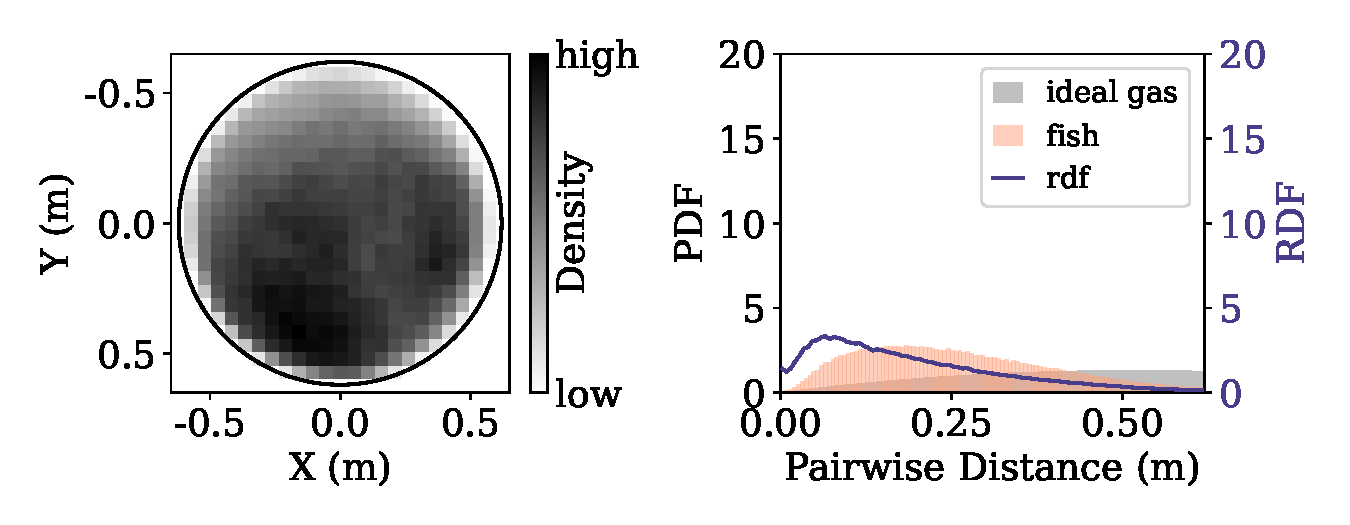
\includegraphics[width=\linewidth]{dist-50-fish}
  \caption[The 2D spatial distribution of 50 fish]{The spatial distribution of 50 adult zebrafish in a quasi 2D environment. Left: the joint distribution of the $X$ coordinates and $Y$ coordinates of the fish positions, with the shape of the boundary being highlighted. Right: the probability density function (PDF) for the distance between two fish. The PDF for the distance of 50 ideal gas particles, uniformly distributed in the tank, were also plotted. The ratio of the two PDFs were taken as the radial distribution function (RDF).}
  \label{fig:density_2d_fish_50}
\end{SCfigure}

\vfill
\pagebreak


\begin{adjustwidth}{0cm}{-5cm}
\begin{tcolorbox}[
fonttitle=\sffamily\Large,
right=0.1\linewidth,
top=5mm,
bottom=5mm,
title=Summary of Chapter~3,
]

\begin{itemize}
	\item Locating a group of fish in 2D is necessary for their 3D reconstruction. For this task, existing methods utilise the morphological details of the fish for identification. These methods are only accurate for fish swimming in a quasi-2D system.
	\item We proposed a new method to locate fish in 2D, where the fish are swimming in a 3D environment. Our method includes the following process.
	\begin{description}
		\item[0. Metric Rectification (optional)] \hfill \\ 
		The distortion and imperfect orientation can be removed by camera calibration.
		\item[1. Image Processing] \hfill \\ 
		The images, captured by the cameras, are separated into the foreground and the background.
		\item[2. Finding Templates] \hfill \\ 
		The individual fish in the foreground are segmented, aligned, and projected to a low dimensional space. Characteristic shapes were identified with clustering algorithm for data points in the low dimensional space.
		\item[3. Constructing the Feature Tensor] \hfill \\ 
		The templates were rotated into different orientations. For every template and orientation, its cross-correlation with the foreground is calculated. The results correspond to a 4D feature tensor.
		\item[4. Extracting the Features] \hfill \\ 
		Local maxima in the 4D feature tensor correspond to the locations, orientations, and shapes of the fish in the image. Each maximum is called a feature in the image.
	\end{description}
	\item We reported the analysis on the coordinates of zebrafish in a quasi-2D environment, featuring different fish numbers.
	\begin{description}
		\item[One Fish] \hfill \\
		The fish tend to swim near the boundary.
		\item[Two Fish] \hfill \\
		The fish tend to swim near one side of the boundary. The heterogeneity of the spatial distribution dominated the radial distribution function.
		\item[Three Fish] \hfill \\
		The behaviour of three adult zebrafish is very similar to that from two fish.
		\item[Fifty Fish] \hfill \\
		The spatial distribution of 50 fish presented a more uniformed manner, with significantly reduced cohesiveness.
	\end{description}
\end{itemize}
\end{tcolorbox}

\end{adjustwidth}

\end{document}
\documentclass[11pt,twoside]{report}
\usepackage{preamble}
\graphicspath{{../img/ch4/}}
\setcounter{chapter}{3}


\begin{document}

\chapter{Observing Zebrafish in 3D}
\label{chapter:fish_3d}

%\epigraph{奇肱之国在其北 其人一臂三目}{\emph{山海经・海外西经}}

\section{Introduction}

This chapter presents the method to build up a system to observe a group of zebrafish in 3D, and obtain the 3D coordinates of individuals in a group of fish. The system is inspired by the pioneering work of \citeauthor{cavagna2008} \cite{cavagna2008} as well as \citeauthor{kelley2013} \cite{kelley2013}, where the 3D locations of European starlings and midges were calculated and analysed. 


The 3D observation is a difficult task. Compared to the the 2D observation introduced in chapter~\ref{chapter:fish_2d}, both the hardware and the software were more complicated for the 3D observation. Typically, we need to use multiple cameras to capture the movement of the fish, where the images were taken in a synchronised way. The calculation also needs more attention, since the optical details, such as the refraction of light at the water--air interface, will affect the final result.


Mathematically, it is important to understand the formation of the image on a camera, because we need to reverse this process to calculate the 3D locations.
For the relevant details, we refer the readers to \cite{hartley2003, ma2005}.
%The relevant details will be covered as a brief introduction of projective geometry in appendix~\ref{chapter:multi_view}. 
This chapter will instead focus on the \emph{implementation} of the ideas.
%Having finished the method section~\ref{section:method_locate_3d}, we should be confident about the calculated 3D locations.
%The accuracy and performance of my software implementation are included in this chapter.
The code responsible for the methods in this chapter is open source, and hosted on website ``GitHub'', with a project name of \href{https://github.com/yangyushi/FishPy}{yangyushi/FishPy}.


It is worth mentioning that the 3D observation method is also widely applied in the study of fluid mechanics \cite{maas1993}, dating back to the 1990s. The name of the method is formally \emph{particle tracking velocimetry}\marginfootnote{
The term ``particle tracking'' in the fluid mechanics community and the soft-matter community refers to slightly different things. The former focus on the dynamic (velocities) of the particles, while the latter focus more on the structure (coordinates) of the particles.
}
(PTV) in the fluid mechanics literatures. Therefore, the new development from the fluid mechanics community may provide opportunity to improve the animal. For instance, by applying the field-programmable gate array (\gls{FPGA}), the 2D feature selection can be performed in real time, which reduced the amount of processing time and data-storage space significantly \cite{chan2007}. 

In addition, the physicists and zoologists have pushed the boundary of technology for field observations. For instance, \citeauthor{cavagna2021} developed the system that can track the 3D movement of animals while moving the cameras with a joypad\marginfootnote{
A joypad is a controller connected to a computer, or other game consoles. In many 3D video games, the players rotate the virtual cameras in the game to explore the environment. This movement is also needed to follow animals in the field.
}, enabling researchers to follow the movement of birds for a long period of time \cite{cavagna2021}.
Another example of advanced observation techniques is the reconstruction of a group of fish in the field, with observers swimming together with the fish, while holding two cameras \cite{francisco2020me}. By incorporation the static environmental information, the movements of the cameras can be effectively estimated, which can be used to reconstruct the trajectories of the fish. 

Using the developed 3D observation system, I studied the behaviour of one adult wildtype zebrafish, as well as groups of zebrafish with different sizes ($N=2, 3, 50$). The result section presents their spatial distribution and the distribution of their pairwise distance. The observed results revealed the important interaction between the fish and the environment. The \emph{dynamic} of the system, which involves the time derivative of the locations, will be analysed and discussed in chapter~\ref{chapter:fish_analysis}.


\section{Methods}
\label{section:method_locate_3d}

This section should serve as a practical tutorial for building a multiple view 3D system to track animals. This system is capable of extracting 3D location of the fish, with three commercial cameras. Our choice is not the only technology to extract 3D information about animals. Instead, there are alternative ways to follow the movement of animals such as binding animals with global positioning system (GPS) \cite{nagy2010} and tagging the animal bodies \cite{jolles2017}. Comparing with these solutions, our method is non-invasive and relatively cheap. However, the obtained results are affected by the errors of the 2D locating of fish individuals (section \ref{section:image_process}), and the ambiguity in the stereo matching process (section \ref{section:fish_many_3d}).

\subsection{Tank Design and Hardware}
\label{section:system_3d}

\begin{SCfigure}
  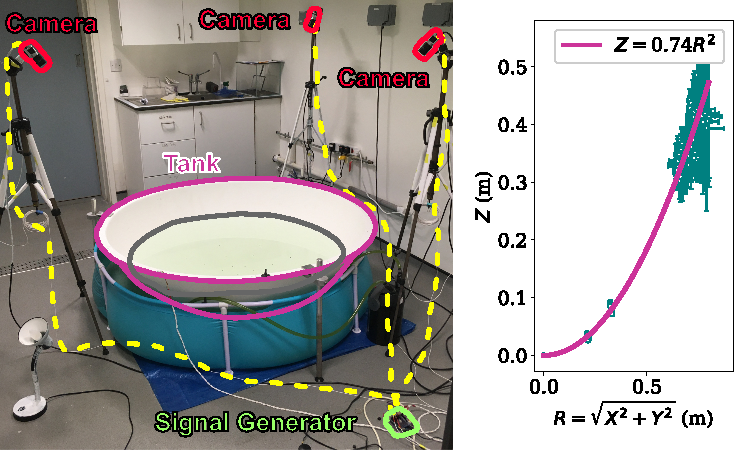
\includegraphics[width=\linewidth]{lab}
  \caption[Three dimensional fish tracking system]{
  Left: The photo of one experimental setup. Three cameras are mounted to observe the fish in the bowl-shaped tank. Time--synchronised signals were generated by an Arduino chip to trigger the cameras for capturing synchronised videos. The bowl was immersed in a bigger tank, which is a framed swimming pool. The husbandry--related equipments, such as the water filter, the heaters, the UV lamp, were placed outside the bowl but inside the bigger tank.
  Right: The measured shape of the observation tank. The scatters were markers on the tank, which were fitted by function $z=0.74 r^2$, where the unit of both $z$ and $r$ is meter.
  }
  \label{fig:lab}
\end{SCfigure}

Figure \ref{fig:lab} shows the experimental setup in the laboratory, where I mounted 3 cameras pointing to a bowl--shaped tank. This big bowl was immersed in a framed swimming pool. Synchronised signals were generated with a Arduino chip, and the cameras are able to capture time--synchronised videos with the signals. The trigger signal for the camera is a 5V pulse, being the default \texttt{HIGH} output signal of an Arduino chip.


The big, white plastic bowl was specially designed and manufactured to contain the fish. The choice of the shape was based on the fact that the fish tend to stay in the corner of the tank, when they entered an unfamiliar environment \cite{kalueff2013, mwaffo2016}. Using a bowl--shaped container prevented the aggregation at the corners. Except for the corner effect, the bowl also provides no blind zone for all of the cameras, preventing the systematic disappear and reappearing of the fish in the video.


%The zebrafish are living animals, and it is also important to provide them a suitable condition. 
In order for the zebrafish to exhibit normal behaviour, they should have water conditions comparable to those used to house them.
Typically, the fish need a temperature between 25 \degree C and 30 \degree C, and the water should be constantly filtered and sterilisation with UV light.
All of the related apparatusse were placed outside the bowl--shaped tank, but inside the swimming pool, so that they would not affect the behaviours of the fish.
The entire system was heated by two commercial heaters. The warm water was circulated into the inner bowl with a water pump. The bowl was able to exchange water with outside via small holes drilled inside. The measured temperature in the swimming pool ranges from 23 \textdegree C to 26 \textdegree C. The water circulation is turned off during observations of fish swimming.


The 3D shape of the tank was measured, so we know the exact boundary for the fish. The measurement was performed by placing markers on the surface of the tank, and then reconstruct the markers in 3D. Since the tank is rotationally symmetric around the z--axis, it is appropriate to describe its geometry in the cylindrical coordinate system with the height ($z$) and the radius ($r$). Figure~\ref{fig:lab} (Right) shows the results of the measurement, and the shape of the tank can be modelled by function $z=0.74 r^2$, where both length variables have the units of meter. The shape of the tank, together with the water level, are the boundaries for the movement of the fish.



\subsection{Locating One Fish in 3D}
\label{section:locate_3d}

\begin{SCfigure}
    \centering
    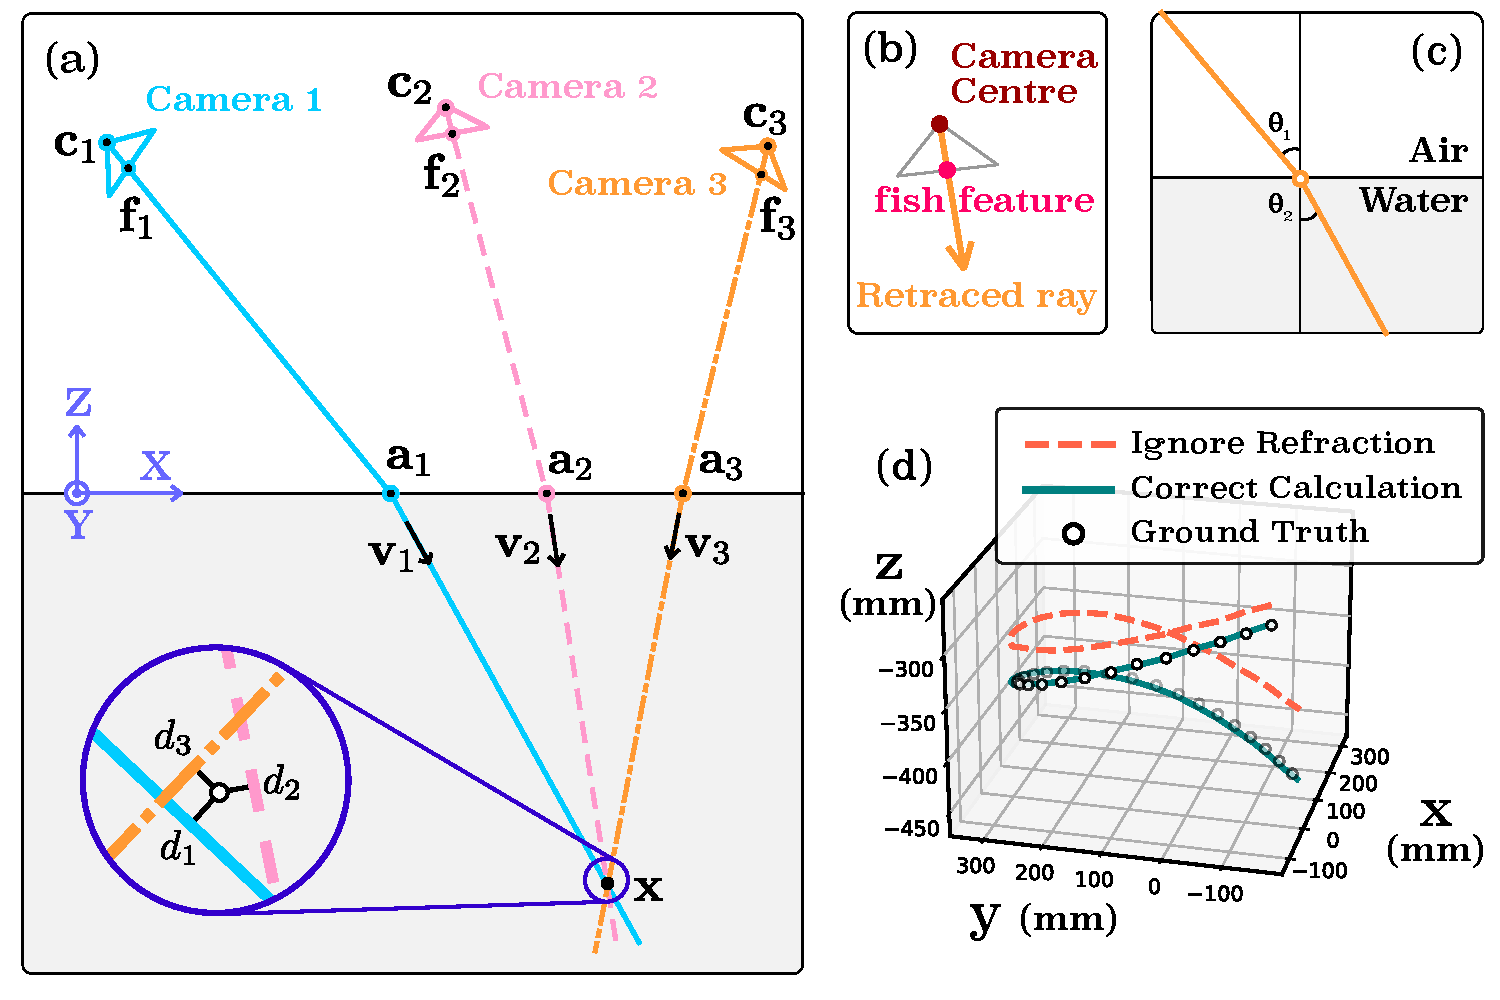
\includegraphics[width=\linewidth]{locate-one}
    \caption[The concept of tracking one fish in 3D]{\label{fig:locate-one}
        The illustrations for the concept for locating one fish in 3D.
        (a) the schematic for the calculation of the 3D fish location from three cameras. The ``intersection'' of the refracted rays were magnified, to stress the retrace distances.
        (b): The illustration of retraced ray from the 2D fish features.
        (c): The effect of the refraction;
        (d): The validation of the calculation for the 3D location of one simulated fish. The solid line is the result where the refraction is considered, and the dashed line is the calculation result that ignored the refraction effect. The scatters represent the ground truth.
    }
\end{SCfigure}



Figure~\ref{fig:locate-one} summarises the essential concept to locate the 3D position with a three camera setup. 
The task of finding the 3D positions of zebrafish consists of two parts. The first part is finding the features of fish in individual cameras, as discussed in the chapter~\ref{chapter:fish_2d}. These features corresponds to $\mathbf{f}_i \in \mathbb{R}^3$ in Fig.~\ref{fig:locate-one}(a).\marginfootnote{
The symbol $\mathbf{f}_i$ stands for the 3D location of the detected 2D features. We need the knowledge of the camera to calculate $\mathbf{f}_i$ from the features in the image. 
}
The second part is to retrace the ray from the features \gls{fi}, back to its original 3D location \gls{xi}, as illustrated in Fig.~\ref{fig:locate-one} (b).

To carry out the 3D calculation procedure, we need to know the location, orientation, and optical details about the camera. This information can be obtained with the \emph{camera calibration} \cite{zhang2000, hartley2003}.
%, which is introduced in appendix~\ref{chapter:multi_view}. 
Essentially, the knowledge of the camera can be represented by a $3 \times 4$ matrix \gls{proj_mat}, named the \emph{projection matrix}. For a 3D point $\mathbf{x} = (x, y, z)^\top$, the camera with projection matrix $\mathbf{P}_{3 \times 4}$ will project the 3D point on a 2D plane, with coordinate $(u, v)^\top$, satisfying  equation,\marginfootnote{I use column vectors consistently in this thesis. For instance, the vector $(x, y, z)^\top$ have the shape of $4 \times 1$; while the vector $(x, y, z)$ have the shape of $1 \times 4$.}

\begin{equation}
	\mathbf{P}_{3 \times 4}
	\cdot (x, y, z, 1)^\top = k (u, v, 1)^\top
\label{eq:projection}
\end{equation}

\noindent where $k$ can take any value.
%(See appendix~\ref{chapter:multi_view} for details)
With proper decomposition of $\mathbf{P}_{3 \times 4}$, it is also possible to calculate the location of the camera centre, illustrated as \gls{center} in Fig.~\ref{fig:locate-one}(a).

 Equation~\ref{eq:projection} suggests an algebraical way to calculate 3D positions from 2D features. With known \gls{proj_mat} and $(u, v)$, Eq.~\ref{eq:projection} offered 2 constrains on the values of \gls{loc3d}. Therefore, the 3D vector $\mathbf{x}$ can be uniquely determined by 2 or more ``camera + feature'' combinations.\marginfootnote{This method to find 3D location is called \emph{triangulation}.} However, the water in the fish tank will refract the light. Figure~\ref{fig:locate-one} (c) shows the effect of refraction, where the angle of incidence $\theta_1$ and the angle of refraction $\theta_2$ follows the Snell's law: $n_1 \sin\theta_1 = n_2 \sin\theta_2$. In our experiment, we have $n_1 = 1$ for the air, and $n_2 = 1.333$ for the water. As a consequence, the calculation of $\mathbf{x}$ involves the following steps,
 
 \begin{enumerate}
 	\item For each feature $\mathbf{f}_i$, calculate its corresponding point on the water-air interface $\mathbf{a}_i$.
 	\item Calculate the direction of refracted ray $\mathbf{v}_i$.
 	\item Find the interception of multiple refracted rays, as the location of fish in 3D $\mathbf{x}$.
 \end{enumerate}


The calculation of \gls{ai} and \gls{vi} requires knowledge of the water-air interface, which was obtained during the camera calibration. Typically, we are free to choose the orientation and location of the \emph{world coordinate frame}. And I set the frame so that the water-air interface is plane $z = 0$, as plotted in Fig.~\ref{fig:locate-one}(a). This extra constrain ensures the value of $\mathbf{a}_i$ being uniquely determined by a 2D feature $(u, v)$. Following Eq.~\ref{eq:projection}:

$$
\left(
\begin{matrix}
	P_{11} & P_{12} & P_{13} & P_{14} \\
	P_{21} & P_{22} & P_{23} & P_{24} \\
	P_{31} & P_{32} & P_{33} & P_{34} \\
\end{matrix}
\right) 
\cdot
\left(
\begin{matrix}
a_x \\ a_y \\ 0 \\ 1	
\end{matrix}
\right) =
k\left(
\begin{matrix}
	u \\ v \\ 1
\end{matrix}
\right),
$$

\noindent where $\mathbf{a}_i = (a_x, a_y)^\mathrm{T}$, and $k$ is a scaling variable that can take any value. Notice there are 3 linear equations for 3 variables ($a_x, a_y$ and $k$), meaning that we can easily calculate $\mathbf{a}_i$. The incident ray can be obtained from $\mathbf{a}_i$ and corresponding \gls{cci}. Applying Snell's law, we can calculate the direction of the refracted ray, yielding $\mathbf{v}_i$. %The algorithm for this calculation is available in appendix~\ref{chapter:algorithms}.


Ideally, the knowledge of the refracted rays ($\mathbf{a}_i$ and $\mathbf{v}_i$) from different cameras yields the 3D location of the fish. Realistically, because of the errors during the 2D feature detection and camera calibration, the retraced rays will not meet each other in 3D space exactly, as pictured in the inset in Fig.~\ref{fig:locate-one}(a). Therefore, finding $\mathbf{x}$ is a minimisation problem. And the value to be minimised is the sum of distances from $\mathbf{x}$ to all the retraced rays. The distance from $\mathbf{x}$ to the retraced ray from camera $i$ is called the \emph{retraced error}, noted as \gls{reterri}. The value of $d_i$ can be calculated as


\begin{equation}
	\label{eq:retrace_err}
	d_i = \vert
	(\mathbf{x} - \mathbf{a}_i) \times \mathbf{v}_i
	\vert,
\end{equation}


\noindent where the retraced ray from camera $i$ passed through point $\mathbf{a}_i \in \mathbb{R}^3$, with the unit direction of $\mathbf{v}_i \in \mathbb{R}^3$. For the constant $\mathbf{a}_i$ and $\mathbf{v}_i$, the squared sum of the retraced error is a function of $\mathbf{x}$, written as,

$$
f(\mathbf{x}) = \sum_i{d_i^2} 
= \sum_i{\left( \vert \mathbf{x} - \mathbf{a}_i \vert^2 \; \vert \mathbf{v}_i^2 \vert - 
\vert \ (\mathbf{x} - \mathbf{a}_i) \cdot \mathbf{v}_i\ \vert^2 \right)}
$$

\noindent where the operator $\vert \cdot \vert$ represents the norm of a 3D vector. We can think of $f(\mathbf{x})$ as a scalar field (like temperature), and the minimum of the field can be found, by setting its gradient ($\nabla f$) to zero. The relation ($\nabla f = 0$) yields a set of linear equations,

\begin{equation}
	\label{eq:location_3d}
	\mathbf{M} \cdot \mathbf{x} = \mathbf{b}.	
\end{equation}

\noindent The values of $\mathbf{M} \in \mathbb{R}^{3 \times 3}$ and $\mathbf{b} \in \mathbb{R}^3$ can be calculated as,

$$
\begin{aligned}
\mathbf{M} &= \sum_i{\mathbf{T}_i} = \sum_i{
\mathbf{v}_i \cdot \mathbf{v}_i^T - 
\textrm{diag}(\mathbf{v}_i \circ \mathbf{v}_i)
} \\
\mathbf{b} &= \sum_i{
\mathbf{T}_i \cdot \mathbf{a}_i,
} \\
\end{aligned}
$$

\noindent where the symbol $\circ$ represents the Hadamard product. The function $\textrm{diag}(\mathbf{x})$ transform the vector $\mathbf{x} \in \mathbb{R}^n$ to a diagonal matrix $\mathbf{D} \in \mathbb{R}^{n \times n}$, where $D_{ii} = x_i$. Solving the equation~\ref{eq:location_3d} is easy with standard linear algebra methods such as Gaussian elimination.\marginfootnote{
Using the Python language, the solution can be found with function \texttt{numpy.linalg.solve(M, b)}. In C++ the task can be performed with \texttt{M.ldlt().solve(b)}, where both \texttt{M} and \texttt{b} are matrix and vector from the \texttt{Eigen} library.
}

Figure~\ref{fig:locate-one} (d) shows the calculation of the 3D location of simulated fish. The simulation was performed with software Blender, in which the experimental apparatus  was constructed virtually. The video was recorded with virtual cameras in the software, and the aforementioned procedure was used to calculate the fish locations. Comparing the calculation result with the known ground truth, it is clear that our calculation yields correct results. 
Since the water is relatively deep (300 - 400 mm in depth) in our experiment, the effect of the refraction could not be ignored. In Fig.~\ref{fig:locate-one} (d) we also present the consequence of ignoring the refraction, which leads to a significant deviation from the ground truth.

\begin{SCfigure}
  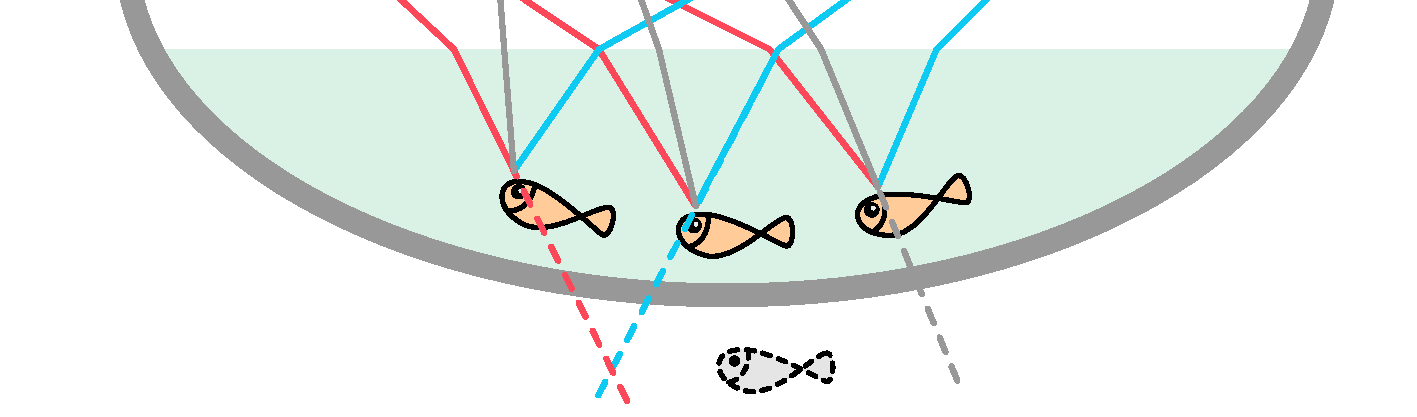
\includegraphics[width=\linewidth]{locate-many}
  \caption[The concept of tracking many fish in 3D]{Tracking many fish with three cameras. The correct identity match from different views yields the intersection between the retraced rays, plotted as solid lines. The unmatched rays will not meet each other, illustrated by the dashed lines.}
  \label{fig:locate-many}
\end{SCfigure}


\subsection{Locating Many Fish in 3D}



Calculating the 3D locations of many fish requires more work than locating one fish in 3D. This is because the different fish in different views (captured by different cameras) have to be matched correctly.
An example of mismatched fish were shown in Fig.~\ref{fig:locate-many} as dashed lines.
Since the three dashed lines correspond to different fish identities, they do not meet together. It is possible to use brute-force enumeration to generate all the possible identities matches, and then discarded the invalid ones. This algorithm was summarised in algorithm~\ref{alg:locate-3d}, where all possible solutions were generated in a triple \code{for} loop. These possible solutions were validated, and the invalid values were discarded.


\begin{algorithm}
    \KwResult{A collection of valid location $\mathbf{x}$}
	\For {$i \gets 1, n_1$} {
	\For {$j \gets 1, n_2$} {
	\For {$k \gets 1, n_3$} {
	$\mathbf{x} \gets $ Solution of $\bf M \cdot x = b$\;
	
	\If {$\mathbf{x}$ is valid}
		{put $\mathbf{x}$ in Result}
	}}}

\caption{Brute force algorithm for locate many fish in 3D.}
\label{alg:locate-3d}
\end{algorithm}


Naively, we will use the retraced error (Eq.~\ref{eq:retrace_err}) to validate every solution $\mathbf{x}$. The operation is summarised in algorithm~\ref{alg:validate-naive}, where a threshold value of $d_m$ is used to discard the solutions with large retraced errors.

\begin{algorithm}

$d_i \gets (\mathbf{x} - \mathbf{a}_i) \times \mathbf{v}_i$\;
$d_j \gets (\mathbf{x} - \mathbf{a}_j) \times \mathbf{v}_j$\;
$d_k \gets (\mathbf{x} - \mathbf{a}_k) \times \mathbf{v}_k$\;
\If {$(d_i + d_j + d_k)/3 < d_m$}
	{\textbf{return} True}
\Else {\textbf{return} False}

\caption{Validate a 3D location with retraced error.}
\label{alg:validate-naive}
\end{algorithm}

However, this method is inadequate because of the correlation of the retraced error and the location of the fish: The retraced error is larger when the fish is deeper in the water. Such correlation is exhibited in Fig.~\ref{fig:compare-error}, with simulated data. The correlation between error values and depth will lead to a systematic error, where the fish closer to the water-air interface will be preferred. Such correlation might originate from the arrangement of the camera. As they were pointed to the water from above, the retraced rays will be closer to each other when they were close to the water-air interface (see Fig.~\ref{fig:locate-many}).

\marginpar{
\centering
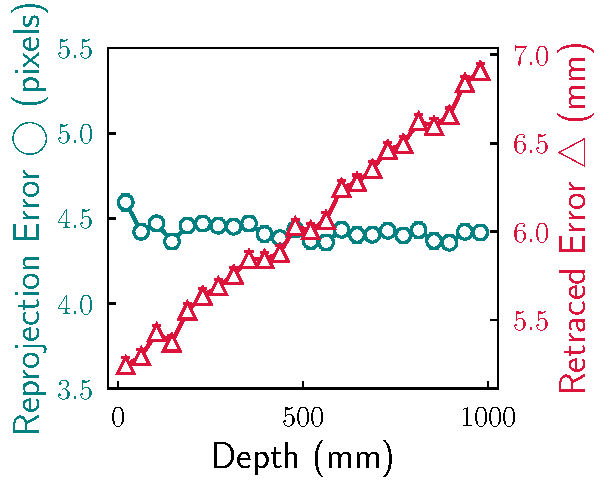
\includegraphics[width=\marginparwidth]{compare-error}
\captionof{figure}[]{
  	The reprojection error ($\epsilon$) and retraced error ($d_i$ in Eq.~\ref{eq:retrace_err}) as a function of fish location.
	}
\label{fig:compare-error}
}

To overcome such bias, we can use the \emph{reprojection error} \cite{hartley2003} to separate the valid and invalid solutions of Eq.~\ref{eq:location_3d}. The reprojection error is defined as

\begin{equation}
	\epsilon_i	= \left\vert 
	( u_\mathbf{x}, v_\mathbf{x} )^\top
	- (u, v)^\top \right\vert
\label{eq:reproj-err}
\end{equation}

\noindent where $(u, v)^\top$ represents the 2D fish features in the camera, and $(u_\mathbf{x}, v_\mathbf{x})^\top$ represents the projection of solution $\mathbf{x}$ to camera $i$. The essential calculation for \gls{reperr} is to re-project a 3D point $\mathbf{x}$ back to the camera correctly, with the optical details being considered explicitly.
%(The calculation for the reprojection is introduced in appendix~\ref{chapter:algorithms}.)
The reprojection error exhibits no correlation with respect to the location of the fish, as shown in Fig.~\ref{fig:compare-error}, which makes it a suitable choice for the validation of fish locations $\mathbf{x}$.\marginfootnote{
Unfortunately, the reprojection error can not be used to find $\mathbf{x}$. The minimisation of $\sum_i\epsilon_i^2$ will not yield a set of linear equations like Eq.~\ref{eq:retrace_err}.
} The algorithm for the validation with the reprojection error is summarised in algorithm~\ref{alg:validate}.


\begin{algorithm}

$\epsilon_i \gets$ reprojection-error($\mathbf{x}$, i)\;
$\epsilon_j \gets$ reprojection-error($\mathbf{x}$, j)\;
$\epsilon_k \gets$ reprojection-error($\mathbf{x}$, k)\;

\If {$(\epsilon_i + \epsilon_j + \epsilon_k)/3 < d_m$}
	{\textbf{return} True}
\Else {\textbf{return} False}

\caption{Validate 3D location with reprojection error.}
\label{alg:validate}
\end{algorithm}



The result of 3D locating of 10 simulated fish were shown in Fig.~\ref{fig:locate-many-valid}. The simulated 3D data were reprojected to different cameras. These projected coordinates were mixed with Gaussian noise, forming the 2D features, to mimic the real life feature measurement. The information of the identity across different cameras was removed. Then our 3D locating method (algorithm~\ref{alg:locate-3d} and \ref{alg:validate}) was used to calculate the 3D locations from these 2D features. It is clear from Fig.~\ref{fig:locate-many-valid} that all of the 10 fish were correctly located, even in the existence of 2D measurement errors.


\begin{SCfigure}
  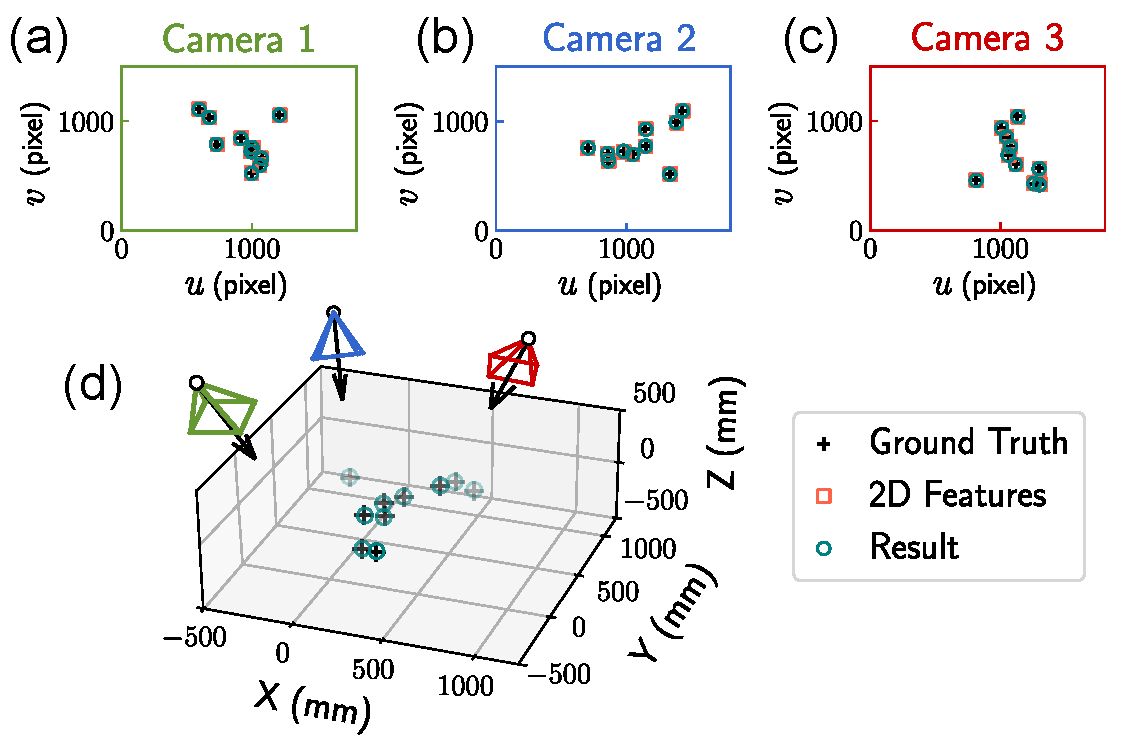
\includegraphics[width=\linewidth]{locate-many-valid}
  \caption[Three dimensional tracking result of simulated data]{
    Calculating the 3D locations of 10 simulated fish locations.
  	(a)-(c): the location captured by different cameras. The cross markers represent the known ground truth. The squares represent the measured 2D features, containing Gaussian noise. The circles represent the projection of the calculated 3D fish locations.
  	(d): the ground truth and the calculated fish location in 3D.
  }
  \label{fig:locate-many-valid}
\end{SCfigure}


\subsection{Optimising the Stereo Matching}
\label{section:stereo-opt}

It is worth mentioning an optimisation idea proposed by \citeauthor{attanasi2015b} to refine the stereo matching of fish identities\marginfootnote{
The same process is called stereoscopic linking in \cite{attanasi2015b}.
}
across different cameras \cite{attanasi2015b}. The idea is to minimise the sum of reprojection error while ensuring the existence of all fish features in the valid solutions. 
For instance, in a collection of valid 3d locations \gls{xijk}, we want to minimise the sum of their corresponding reprojection errors (Eq.~\ref{eq:reproj-err}), by discarding some ``bad'' solutions. The result of this process is a subset of \gls{xijk}, noted as \gls{xijkopt}.
And the solutions in \gls{xijkopt} are termed as the \emph{optimised solutions}.

Without any constraint, the result of minimised error will be an empty set, meaning $\{ \mathbf{x}_{ijk} \}_\textrm{opt} = \emptyset$. This is not very effective because the algorithm will trivially return nothing. A sensible way to remedy this situation is to enforce some kind of constraint, to ensure the existence of good results. The essence of the idea from \citeauthor{attanasi2015b}, is the following constraint,

$$
\forall i \; \sum_{j k} x_{i j k} \geq 1,
\forall j \; \sum_{k i} x_{i j k} \geq 1,\;\textrm{and}\;
\forall k \; \sum_{i j} x_{i j k} \geq 1,
$$

\noindent where $i, j, k$ are the indices for features in the 3 cameras. The symbol $x_{ijk}$ represents a 3D boolean tensor, whose elements can take values of $0$ or $1$. If the value of $x_{ijk} = 1$, then the feature $i$ in camera 1, the feature $j$ in camera 2, and the feature $k$ in camera 3 will form a optimised solution (in $\{ \mathbf{x}_{ijk} \}_\textrm{opt}$). Formally, the task can be written as a \emph{linear programming} problem, written as,

\begin{equation}
\begin{aligned}
	\textrm{Minimize} 
	&& \sum_{ijk}{\epsilon_{ijk}} \\
	\textrm{Subject to}
	&& \forall i \; \sum_{j k} x_{i j k} \geq 1, \\
	&& \forall j \; \sum_{k i} x_{i j k} \geq 1 \\
	&& \forall k \; \sum_{i j} x_{i j k} \geq 1
\end{aligned}
\label{eq:stereo-opt}
\end{equation}

\noindent This problem can be solved effectively by modern optimisation libraries, and they give satisfying results without significant increase in the computation time.


\begin{tcolorbox}[
title=What is ``Linear Programming'',
enlarge bottom by=0.5em,
enlarge top by=0.5em,
parbox=false
]
The method \emph{linear programming} is a very useful optimisation method. We can use it to find the maximum value of a function, plus a set of linear constraints. Equation~\ref{eq:stereo-opt} is an example of the problem that linear programming could solve. To actually solve the problem, we need to apply some complicated algorithms like the \emph{simplex algorithm}. The details of these algorithms are beyond the scope of this thesis.

Practically, we can use many existing libraries and softwares to solve the linear programming problems. I used the CPLEX package from the company IBM to carry out the linear programming calculation, following \cite{attanasi2015b}. The package is not open-source, but offers free academic licence for researchers. Being a powerful solver, the CPLEX package can solve optimisation problems with quadratic constraints. We will utilise this feature in chapter~\ref{chapter:fish_analysis} to remove overlapping particles.

Confusingly, the ``programming'' in the name does not refer to computer programmes. It originates from its first application, where George B. Dantzig was invited to solve an assignment problem for American military after world war II \cite{dantzig2002}. Internally, the schedules in the army was called the programme. \citeauthor{dantzig2002} formulated the problem into a system of linear inequalities, and published a paper under the name of \emph{Programming in a Linear Structure}. Later, he took the suggestion from a friend, and changed the name of this method to \emph{linear programming}, while strolling on the Santa Monica beach in the summer of 1948 \cite{dantzig2002}.
\end{tcolorbox}


\subsection{Assessing the Algorithm}

For the experimental videos, the realistic accuracy of the algorithm depends on the distribution of the 2D error as well as the error in the camera calibration process.
It is difficult to estimate the effects of theses uncertainties theoretically, and we refer the readers to \cite{theriault2014} for relevant studies.

Practically, we can inspect the reprojected locations $(u_\mathbf{x}, v_\mathbf{x})$ to check the accuracy.
An example is shown Fig.~\ref{fig:locate-performance} (a), where the reprojected 3D tracking result as well as the detected 2D features were plotted on top of the captured image from one camera.
The distribution of the reprojection error $\epsilon$ was plotted in Fig.~\ref{fig:locate-performance} (c), featuring a peak at $\sim$ 2 pixels.
The distribution of $\epsilon$ indicates that the reprojected coordinates $(u_\mathbf{x}, u_\mathbf{x})$ are close to the 2D features $(u, v)$.
Such proximity should give us confidence about the algorithm on the experimental data. Notably, the 3D locating algorithm is even capable of discarding some invalid 2D features, since their corresponding invalid 3D result would be discarded by algorithm~\ref{alg:validate}.


\begin{SCfigure}
  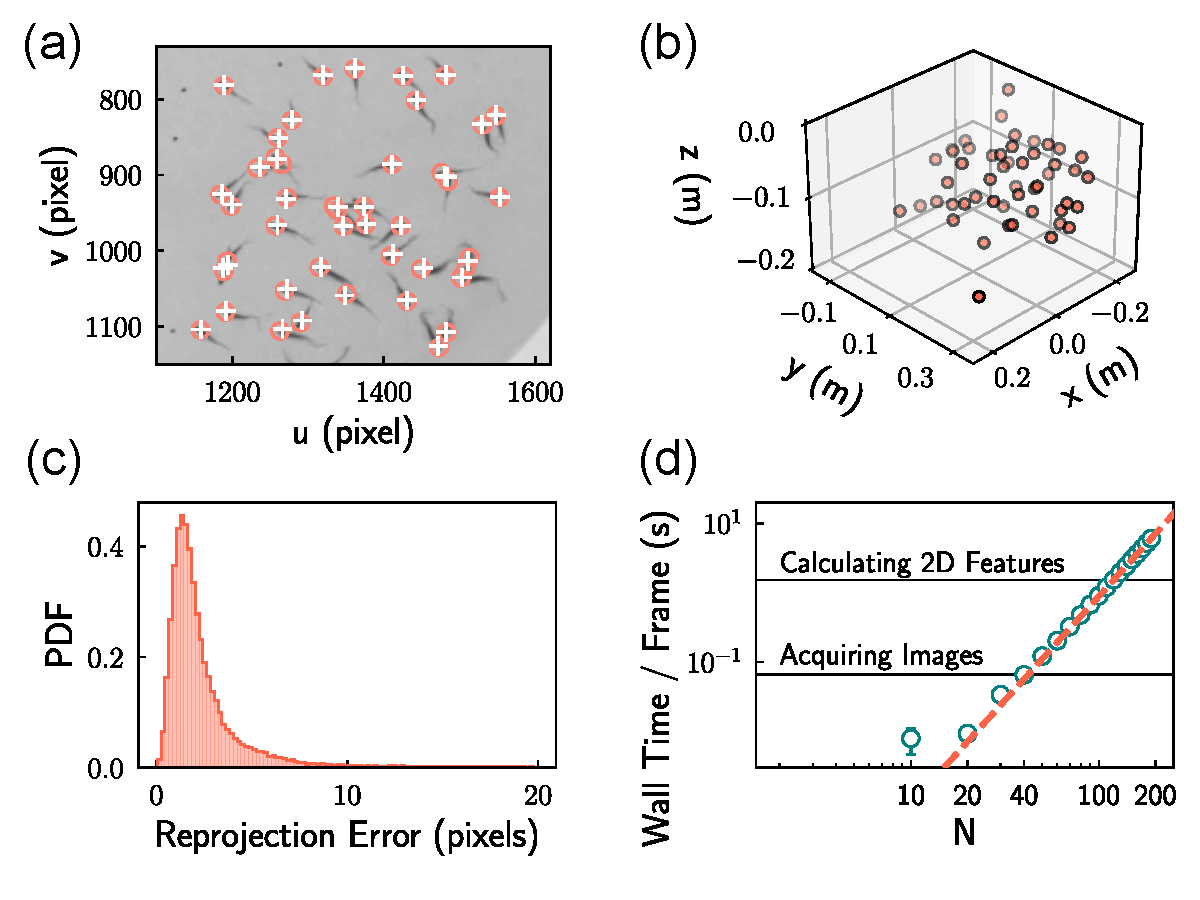
\includegraphics[width=\linewidth]{locate-perform}
  \caption[Performance of the 3D locating method]{
  (a) An image of 40 zebrafish in the experimental setup.  The detected 2D features, corresponding to $(u, v)$ in Eq.~\ref{eq:reproj-err}, were plotted as white circles. The reprojected 3D tracking result, corresponding to $(u_\mathbf{x}, v_\mathbf{x})$ in Eq.~\ref{eq:reproj-err}, were plotted as the red cross markers. We cropped the image to focus on the fish group. 
  (b) The reconstructed 3D locations of 40 zebrafish from three different cameras.
  (c) The distribution of reprojection error $\epsilon$.
  (d) The wall time of the 3D locating algorithm for different numbers of fish. The dashed line shows the cubic fitting ($y = a x^3 + b$).
  }
\label{fig:locate-performance}
\end{SCfigure}


The complexity of the 3D locating algorithm is $\mathcal{O}(n^3)$, because of the triple \code{for} loop in algorithm~\ref{alg:locate-3d}. The performance of the algorithm is shown in Fig~\ref{fig:locate-performance} (d), where the wall time\marginfootnote{
The wall time refers to time spent in real life, counted by a clock on the ``wall''
} exhibits the expected cubic increase.
 To get even better performance, one needs to improve the algorithm to reduce the complexity from $\mathcal{O}(n^3)$. A possible option is to exploit the epipolar geometry \cite{hartley2003}, which can reduce the complexity of the algorithm. Further optimisation of the 3D locating algorithm will be an important task of this project in the future.


Even though the 3D locating algorithm was not optimised, it is good enough\marginfootnote{
To achieve high performance, a fast programming language is important: the result in Fig.~\ref{fig:locate-performance} was from an implementation using the C++ language, which is 1,000 times faster than a Python implementation.
} for relatively small group sizes (less than 100 fish).
For these small numbers, the bottleneck of the calculation is the 2D feature detection, which took about 2s for each frame.
With an image acquisition frequency of 15 FPS, the 3D locating calculation for group size $<$ 40 can even be performed in real time, if the 2D feature calculation time can be decreased dramatically.



\section{Results}
\label{section:observe-3d-result}

The 3D tracking yields the positions of the fish. From the positions, we can estimate the spatial distribution, and measure the structure of a group of fish.


\subsection{A Single Fish}
\label{section:fish_1_3d}


Figure~\ref{fig:density_3d_fish_1} (a) shows the joint probability density function (\gls{PDF}) of the $x$ and $z$ coordinates of the fish, noted as \gls{pdfxy}. This spatial distribution shows that the fish tend to stay in the bottom of the tank. We observe this behaviour repeatedly, when the fish were subjected to a new environment. It is likely to be related to the ``depth preference'' of zebrafish \cite{kalueff2013}, where the fish prefer deep water naturally. In addition, the increasing anxiety would also drive the fish to go to the bottom of the tank \cite{cachat2011, cachat2019}.


The distribution of the planer radius, $r=\sqrt{x^2 + y^2}$ is shown in Fig.~\ref{fig:density_3d_fish_1} (b), noted as $f_R(r)$. The shape of \gls{pdfr} is affected by the geometry of the tank. To understand the effect of this boundary, we calculated the distribution of the ideal gas particles, distributed uniformly inside the fish tank (see chapter~\ref{chapter:fish_model} for details). Compared to the ideal gas particles, the distribution of $r$ is closer the the centre. The shifted distribution of the fish is related to their depth preference, since the fish will be forced to the central region of the tank as they swim deeper in the water.
There are two peaks in $f_R(r)$, and this bimodal feature can be explained by the holes drilled on the tank, which will be discussed in section~\ref{section:holes}.

The distribution of $z$ component of the coordinate of the fish, noted as \gls{pdfz}, is shown in Fig.~\ref{fig:density_3d_fish_1} (c), which presents a very sharp peak around $z = 0$ m.
To get a better understanding of the fish, we calculated the \emph{excess probability density function}, \gls{pdfexz}, as

\begin{equation}
	f_Z^\mathrm{ex}(z) = \frac{f_Z^\mathrm{fish}(z)}{f_Z^\mathrm{id}(z)}
\label{eq:dist_excess}
\end{equation}

\noindent where the term $f_Z^\mathrm{fish}(z)$ represents the height distribution of the fish, while $f_Z^\mathrm{id}(z)$ represents the distribution of the ideal gas particles. The logarithm of $f_Z^\mathrm{ex}(z)$ is shown in Fig.~\ref{fig:density_3d_fish_1} (d), featuring a linear decay of the peak, and a subsequent tail.
This initial exponential decay is surprising, and it is reminiscent of the height distribution of one colloidal particle, under the gravitational field \cite{biben1993, royall2007prl}.  
We can fit this exponential decay with the following function,

\begin{equation*}
f_Z^\mathrm{ex}(z) = a \exp\left( \frac{z}{\xi_g} \right)
\end{equation*}

\noindent where $a$ is free parameter, and \gls{xig} is a length scale related to the depth preference of the fish. The value of $\xi_g$ is a measure of the ``effective gravity'' exhibited by fish, that is related to its depth preference. For one adult zebrafish, the value of $\xi_g$ is 1.2 cm. The effective gravity for the fish will be further discussed in chapter~\ref{chapter:fish_model}.


\begin{SCfigure}
  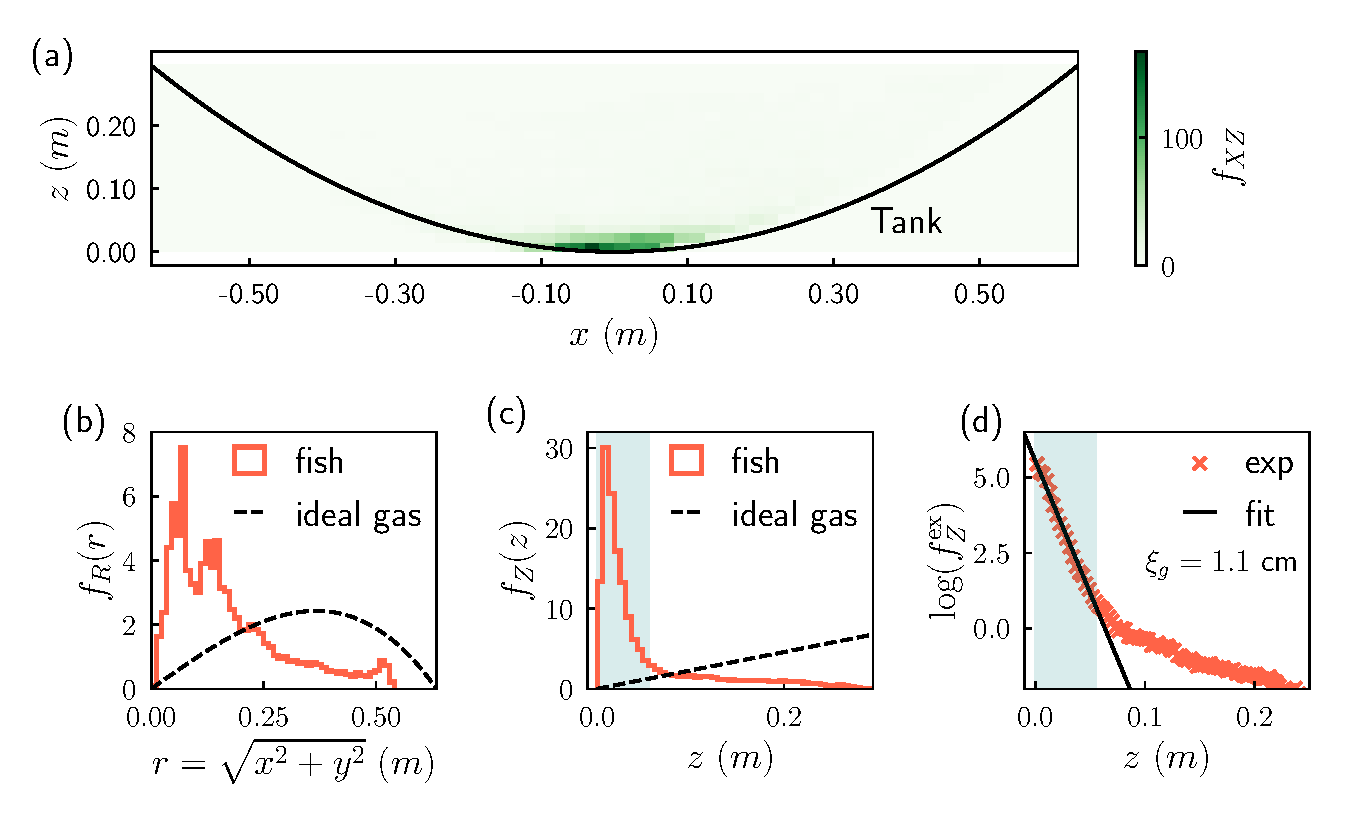
\includegraphics[width=\linewidth]{density-one-fish}
  \caption[The 3D spatial distribution of one fish]{
  The spatial distribution of one zebrafish.
  (a) The joint probability density function of $x$ and $z$ components of the fish.
  (b) The PDF for the planer radius $r$ of the fish. The dashed line shows the same PDF for the ideal gas particles distributed uniformly in the tank.
  (c) The PDF for the $z$ component of the fish. The dashed line shows the same PDF for the ideal gas particles distributed uniformly in the tank.
  (d) The semi-log plot of the excess PDF, $f_Z^\mathrm{ex}$ in Eq.~\ref{eq:dist_excess}, for the $z$ component for the fish. Fitting its initial decay revealed a lengthscale of 1.1 cm. The region of the initial decay is heighlighted in (c) and (d).
}
  \label{fig:density_3d_fish_1}
\end{SCfigure}


\subsection{Two Fish}
\label{section:fish_2_3d}


The spatial distribution of 2 zebrafish is presented in Fig~\ref{fig:density_3d_fish_2}. The behaviour of two fish is similar to that of one fish, exhibiting the typical depth preference. However, the distribution of two fish is broader compared to that of one fish.
The broader distribution indicates an increased randomness, which might related to the a decreased level of anxiety\marginfootnote{
To the best of my knowledge, there is no direct proof to suggest that zebrafish perceive less danger in a larger group. It is a reasonable speculation, since zebrafish form  groups naturally in the wild \cite{shelton2020}.
}, as the fish were swimming in pairs. In other words, one fish might be very vigilant in a new environment, exhibiting the anxiety-driven depth preference \cite{cachat2011}, which leads to a narrow distribution of $f_Z(z)$. For a pair of fish, this depth preference was reduced. The fitting result of $f_Z^\mathrm{ex}(z)$ yields a $\xi_g$ value of 1.8 cm, which is larger than the $\xi_g$ value of one fish (1.2 cm), as a result of reduced depth preference.

\begin{SCfigure}
  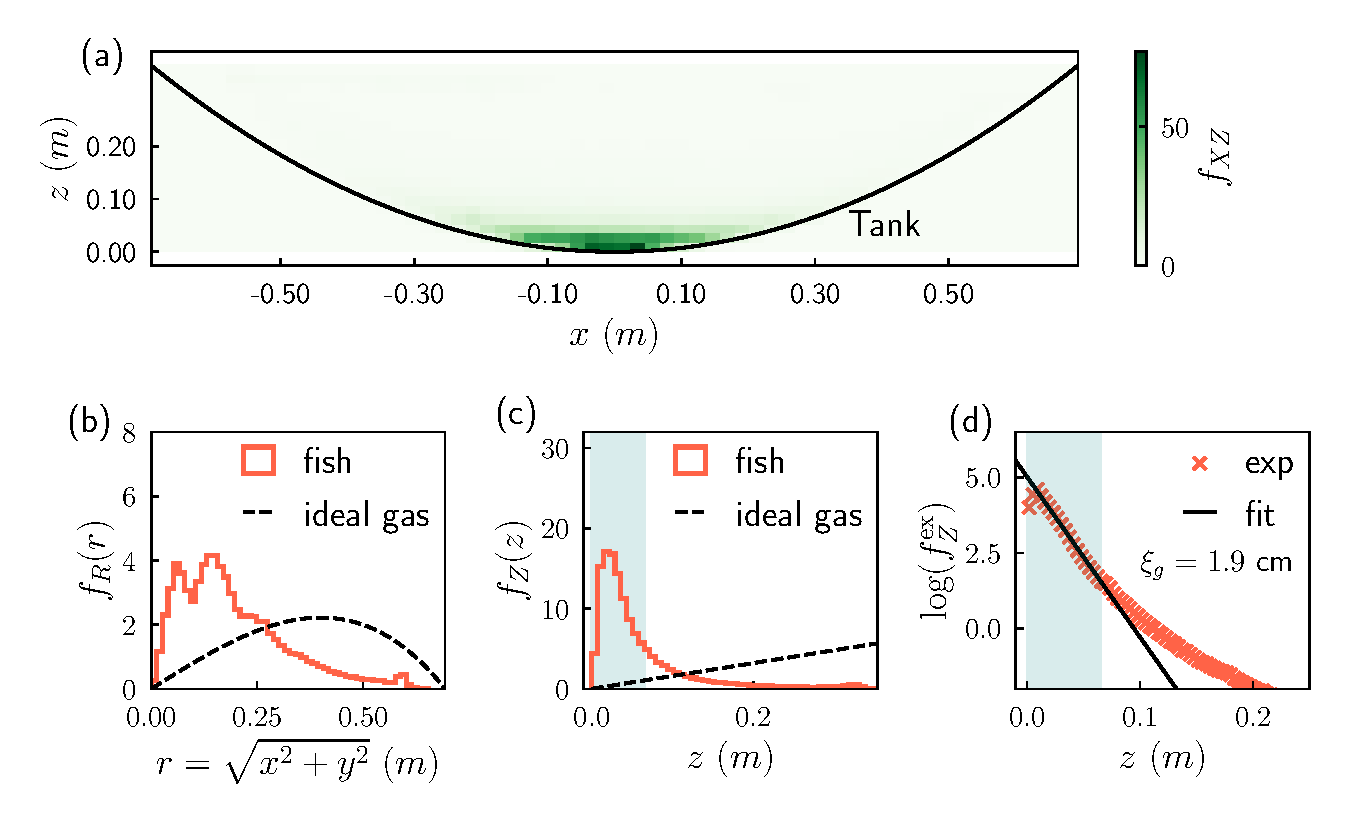
\includegraphics[width=\linewidth]{density-two-fish}
  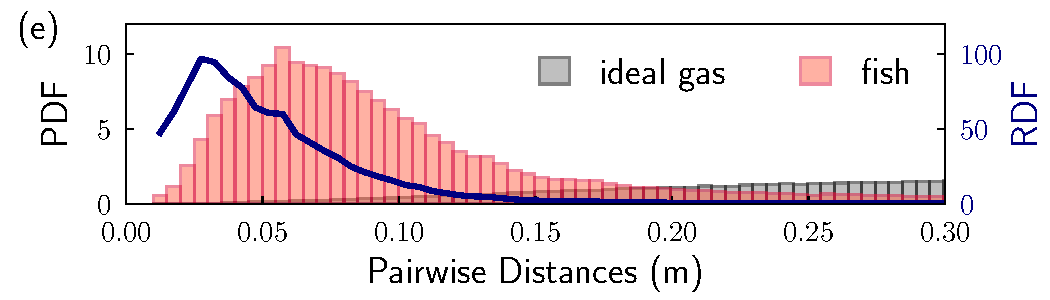
\includegraphics[width=0.9\linewidth, outer]{pdist-2fish}
  \caption[The 3D spatial distribution of two fish]{
  The spatial distribution of two adult zebrafish.
  (a) The joint probability density function of $x$ and $z$ components of the fish.
  (b) The PDF for the planer radius $r$ of the fish. The dashed line shows the same PDF for the ideal gas particles distributed uniformly in the tank.
  (c) The PDF for the $z$ component of the fish. The dashed line shows the same PDF for the ideal gas particles distributed uniformly in the tank.
  (d) The semi-log plot of the excess PDF, $f_Z^\mathrm{ex}$ in Eq.~\ref{eq:dist_excess}, for the $z$ component for the fish. Fitting its initial decay revealed a lengthscale of 1.9 cm. The region of the initial decay is heighlighted in (c) and (d).
  (e) The PDF of pairwise distances of the fish and the ideal gas particles in the tank. The ratio of the two, the radial distribution function (RDF), is plotted as a solid line.
  }
  \label{fig:density_3d_fish_2}
\end{SCfigure}

The fish-fish interaction can be probed by the distribution of the pairwise distances as well as the radial distribution function (RDF), as discussed in chapter~\ref{chapter:fish_2d}. The probability density function (PDF) of the pairwise distance of 2 fish was shown in Fig.~\ref{fig:density_3d_fish_2}, along with the corresponding PDF of the ideal gas particles uniformly distributed in the fish tank. The PDFs of the fish distance exhibit a peak around 5 cm, which is dominated by the inhomogeneity of the density distribution.

The RDF of 2 fish in the system exhibits a peak around 0.03m, with a hight\marginfootnote{
For the densely packed fluid, like a collection of hard spheres at volume fraction of 54\%, the peak height is $\sim 6$.
} value of $\sim$ 100. The hight value is significantly larger, comparing with the RDF peak height ($\sim 15$) of 2 fish in 2D.
However, this does \emph{not} imply the fish were swimming in a more cohesive fashion in 3D. Instead, 
the RDF describes the depth preference of the fish, which generated significant density inhomogeneity, illustrated in Fig.~\ref{fig:density_2d_fish_2} (a).
In other words, the fish appear to swim together in a more cohesive fashion in 3D, according to the numerical value of the RDF. But the cohesion was not driven by the (biological) fish-fish attraction.
Instead, these fish were just bounded together by their interaction with the environment, i.e. the depth preference.
This bias induced by the depth preference can be corrected with advanced sampling method, which will be covered in chapter~\ref{chapter:fish_analysis}.


\subsection{Three Fish}
\label{section:fish_3_3d}

The spatial distribution of 3 zebrafish is presented in Fig~\ref{fig:density_3d_fish_3}. Being similar to the 1-fish and 2-fish system, a group of 3 zebrafish presents the depth preference, indicated by the biased joint PDF of $z$ and $z$ components of the fish coordinates. The PDFs ($f_Z(z)$, $f_R(r)$, and $f_{XZ}$) of 3 fish is very similar to the results from 2 fish experiments. This similarity was also observed in the 2D experiments (section~\ref{section:fish_2_2d}).

The distribution of the pairwise distance of 3 zebrafish exhibits one peak around 0.08m. The length scale matched the size of the high-density blob in Fig.~\ref{fig:density_3d_fish_3} (a), thanks to the depth preference of the fish. The RDF of 3 fish is similar to the RDF of 2 fish, with a peak at around 0.03 m. The height of the peak is close to 100, due to the depth preference of the fish, as discussed in section~\ref{section:fish_2_3d}.

\begin{SCfigure}
  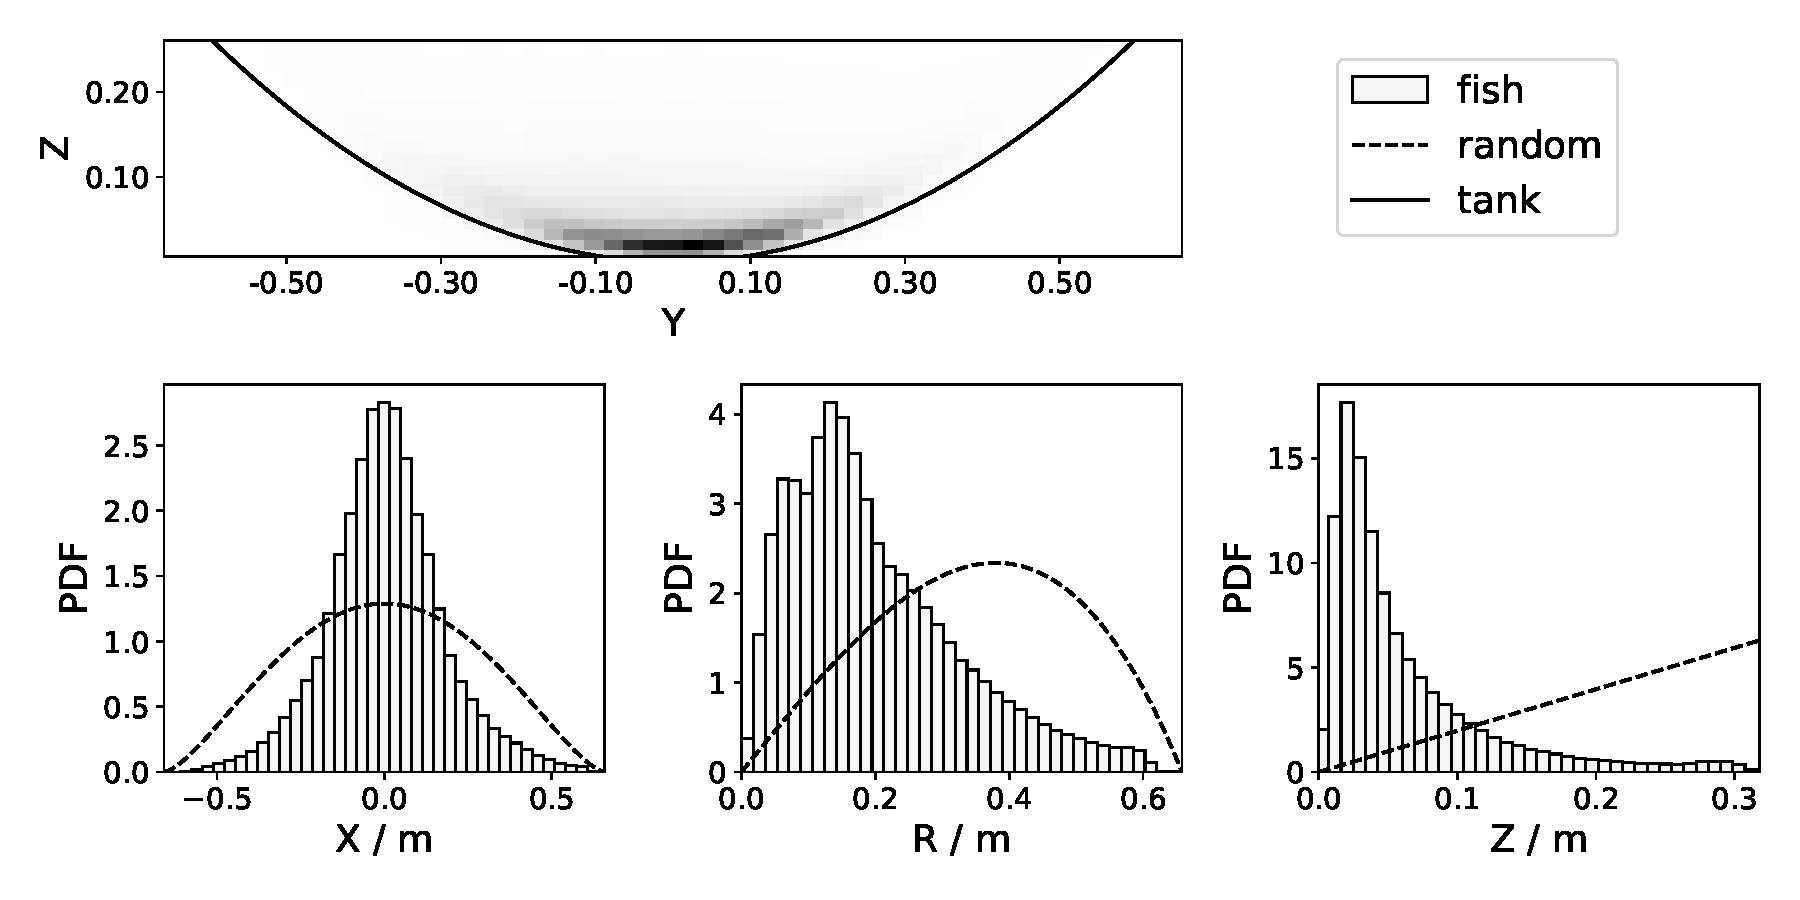
\includegraphics[width=\linewidth]{density-three-fish}
  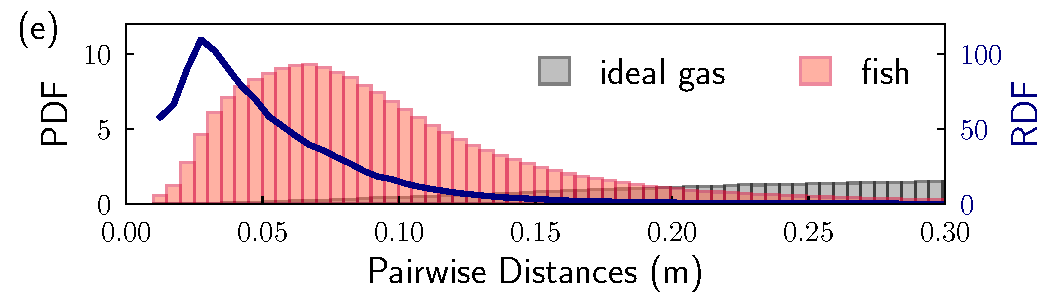
\includegraphics[width=0.9\linewidth, outer]{pdist-3fish}
  \caption[The 3D spatial distribution of three fish]{
  The spatial distribution of three adult zebrafish. 
  (a) The joint probability density function of $x$ and $z$ components of the fish.
  (b) The PDF for the planer radius $r$ of the fish. The dashed line shows the same PDF for the ideal gas particles distributed uniformly in the tank.
  (c) The PDF for the $z$ component of the fish. The dashed line shows the same PDF for the ideal gas particles distributed uniformly in the tank.
  (d) The semi-log plot of the excess PDF, $f_Z^\mathrm{ex}$ in Eq.~\ref{eq:dist_excess}, for the $z$ component for the fish. Fitting its initial decay revealed a lengthscale of 1.8 cm. The region of the initial decay is highlighted in (c) and (d).
  (e) The PDF of pairwise distances of the fish and the ideal gas particles in the tank. The ratio of the two, the radial distribution function (RDF), is plotted as a solid line.
  }
  \label{fig:density_3d_fish_3}
\end{SCfigure}


\subsection{Many Fish}
\label{section:fish_many_3d}

Figure~\ref{fig:density_3d_fish_50} shows the spatial distribution of 50 adult zebrafish, as well as the distribution of their pairwise distances and the RDF. The depth preference is obvious for a group of 50 fish, as shown in the joint PDF of $x$ and $z$ components of the fish coordinates.
However, the distribution is more homogeneous comparing with the 1/2/3 fish results. This homogeneity could be the result of reduced depth preference, as the $\xi_g$ value for 50 zebrafish is larger than that of the 1/2/3 fish. Biologically, the reduction of depth preference (the increase of $\xi_g$) can be explained by our assumption, that the fish perceive less danger in a larger group.

The distribution of the $z$ component, interestingly, exhibits two separated peaks. One of the peak is close to $z = 0\ m$ which can be explained with the depth preference. The other peak is located at $z = 0.35\ m$, which corresponds to the top of the tank. This suggests the fish were also attracted by the water-air interface. Such bimodal distribution is likely due to the biological preference of the fish, which will be further analysed in chapter~\ref{chapter:fish_analysis}.

The 50 zebrafish also shows a broad distribution for their pairwise distances. This can be explained by the reduced density inhomogeneity of the fish. Consequently, the group of 50 fish appears to be less cohesive, indicated by the absence of sharp peak in their RDF, as shown in the bottom panel of Fig.~\ref{fig:density_3d_fish_50}. The observation that a large group of fish exhibits less cohesion and less spatial inhomogeneity, was also captured by the 2D fish experiments shown in section~\ref{section:fish_50_2d}.


\begin{SCfigure}
  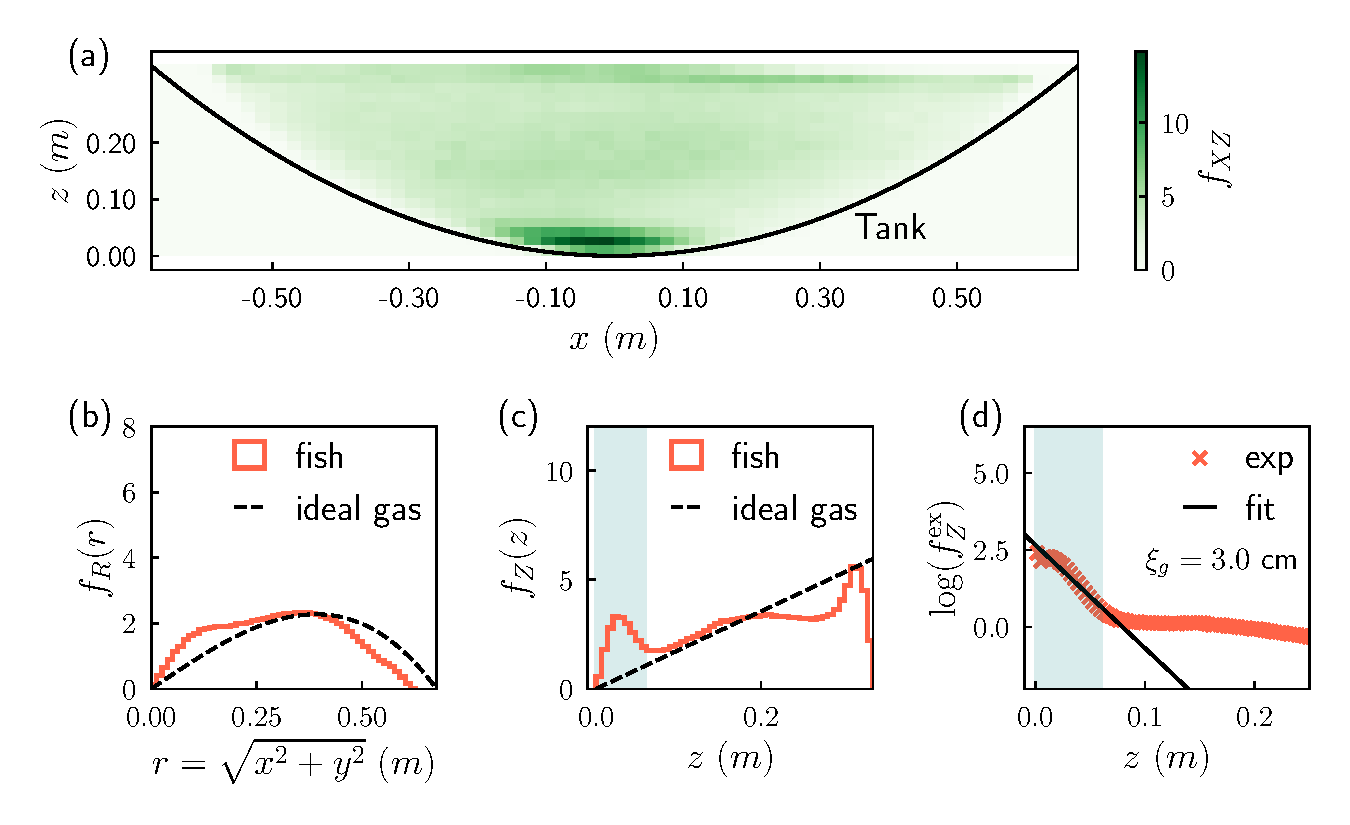
\includegraphics[width=\linewidth]{density-fifty-fish}
  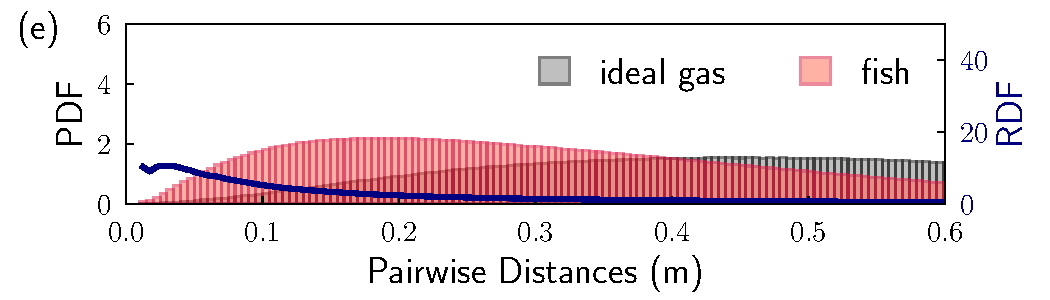
\includegraphics[width=0.9\linewidth, outer]{pdist-50fish}
  \caption[The 3D spatial distribution of 50 zebrafish]{
  The spatial distribution of fifty adult zebrafish. 
  (a) The joint probability density function of $x$ and $z$ components of the fish.
  (b) The PDF for the planer radius $r$ of the fish. The dashed line shows the same PDF for the ideal gas particles distributed uniformly in the tank.
  (c) The PDF for the $z$ component of the fish. The dashed line shows the same PDF for the ideal gas particles distributed uniformly in the tank.
  (d) The semi-log plot of the excess PDF, $f_Z^\mathrm{ex}$ in Eq.~\ref{eq:dist_excess}, for the $z$ component for the fish. Fitting its initial decay revealed a lengthscale of 3.0 cm. The region of the initial decay is highlighted in (c) and (d).
  (e) The PDF of pairwise distances of the fish and the ideal gas particles in the tank. The ratio of the two, the radial distribution function (RDF), is plotted as a solid line.

  }
  \label{fig:density_3d_fish_50}
\end{SCfigure}


\subsection{The Holes on the Tank}
\label{section:holes}

\marginpar{
\centering
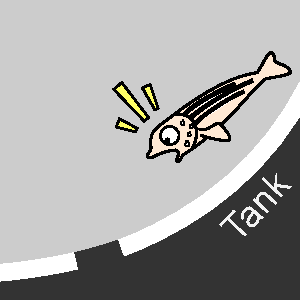
\includegraphics[width=\marginparwidth]{hole}
The holes on the tank affected the zebrafish.
}

The holes drilled on the surface of the tank had an unexpectedly large effect on the spatial distribution of the zebrafish. These holes were designed for the circulation of the water in the tank. They appear as black dots in Fig.~\ref{fig:density-holes} (right). However, the location of these holes matched the $R$ values of the density distribution, where the discontinuous singularity happens, as shown in Fig~\ref{fig:density-holes} (left). This indicates that the fish actively avoids swimming on top of these holes.

For the distribution of 1 fish, the fish-hole interaction is very significant, indicated by a very clear separation of peaks around $R=0.1$. Such separation is less significant in from the result of 2 fish and 3 fish experiments. For 50 fish, the effect of the holes is not observed in Fig.~\ref{fig:density-holes}. The result is consistent with the observation in 2D, were the fish-tank interaction dominates the 1/2/3 fish behaviour, while the fish-fish interaction dominates the behaviour of 50 fish. Such observation indicates the necessity for the large group animal behaviour experiments, if we are interested in the interaction between animal individuals.

This information about the fish-tank interaction is important for the purpose of the modelling. In chapter~\ref{chapter:fish_model} we will show that a small group of fish can be modelled as a system in equilibrium with pairwise interaction, under the influence of the tank, the gravity, as well as the holes. The Boltzmann energy weight, as a result of our equilibrium assumption for the system, gives a good match for the observed spatial distribution.


\begin{SCfigure}
  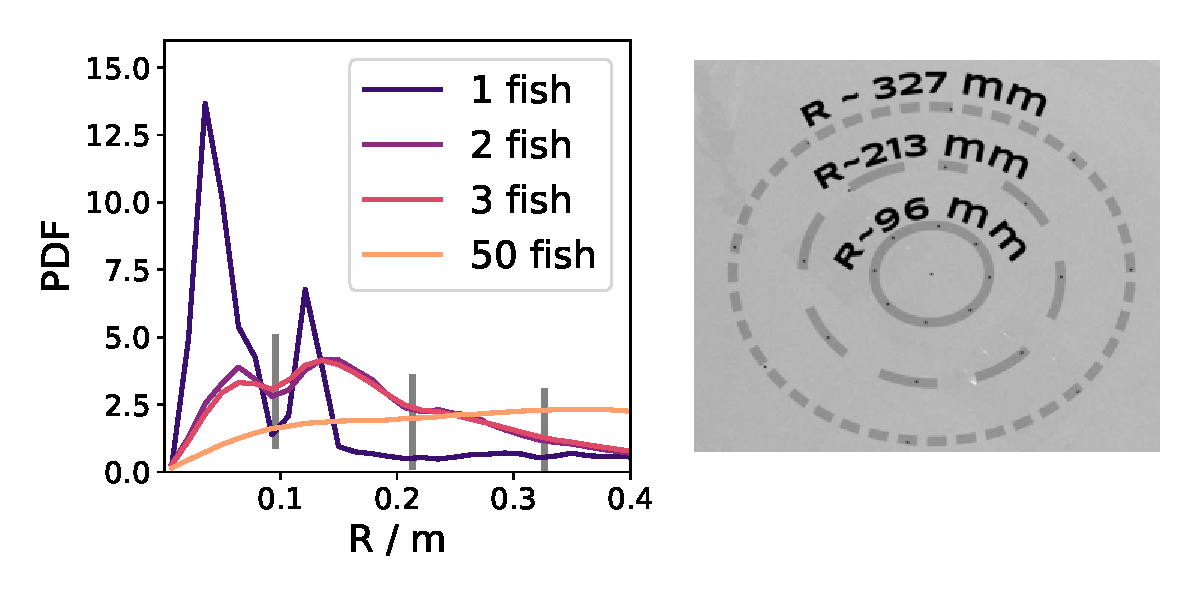
\includegraphics[width=\linewidth]{density-hole}
  \caption[The effect of drilled holes on the tank on the spatial distribution of the fish.]{
  	Left: the distribution of the planar radius ($R$), where the location of the drilled holes were marked with vertical lines.
  	Right: a photo of the bottom of the fish tank, highlighting the location and planar radius of the holes.
  }
  \label{fig:density-holes}
\end{SCfigure}

\vfill
\pagebreak

%\section{Conclusion}
%
%This chapter provides an introduction for the calculation of fish location in 3D from a multiple view system. The methods section gives an overview of the hardware design as well as the software design. Especially, the mathematical basis as well as the algorithm for the 3D locating problem is given explicitly, where the reader should be able to understand and implement a similar software for the same task. The performance and accuracy of my implementation was reported, suggesting the code is capable of processing a relatively large ($n \sim 50$) group of fish.
%
%Using the developed hardware and software, I present the spatial distribution of 1/2/3 and 50 fish. These distribution were inhomogeneous, being similar to the results observed in the quasi-2D experiment reported in chapter~\ref{chapter:fish_2d}. Surprisingly, the fish responded strongly to the small holes drilled in the tank, leading to characteristic peak split in the marginal distribution of the planar radius of the fish. For 50 fish, the interaction between the fish and the holes were not observable, indicating the behaviour of 50 were dominated by the fish-fish interaction. The interaction between the fish and the environment, otherwise, contributes significantly to the 1/2/3 fish behaviour.

\begin{adjustwidth}{0cm}{-5cm}
\begin{tcolorbox}[
fonttitle=\sffamily\Large,
right=0.1\linewidth,
top=5mm,
bottom=5mm,
title=Summary of Chapter~4,
]

\begin{itemize}
	\item Locating fish in 3D requires synchronised images from different cameras. We Presented the experimental setup for this task.
	\item We introduced the idea to calculate the 3D location of one fish from its corresponding 2D features from different cameras.
	\item We presented a brute-force algorithm to locate multiple fish in 3D, highlighting the importance of the reprojection error. We also introduced the optimisation of the result with the help of linear programming. The accuracy and complexity of the multiple-fish locating algorithm is assessed.
	\item We reported the analysis on the coordinates of zebrafish in a 3D environment, featuring different fish numbers.
	\begin{description}
		\item[One Fish] \hfill \\
		The fish tend to swim near the bottom of the tank. The height distribution exhibit an exponential decay, featuring the depth preference of the fish, which can be characterised by a length scale $\xi_g$.
		\item[Two Fish] \hfill \\
		The fish tend to swim near the bottom of the tank, with slightly increased $\xi_g$ value, suggesting a reduced depth preference. The depth preference dominated the radial distribution function.
		\item[Three Fish] \hfill \\
		The behaviour of three adult zebrafish is very similar to that from two fish.
		\item[Fifty Fish] \hfill \\
		The spatial distribution of 50 fish is more uniform, compared to the 1/2/3 fish results. As a result, the RDF of 50 zebrafish shows significantly reduced cohesiveness.
	\end{description}
	\item Surprisingly, the fish responded strongly to the small holes drilled on the surface of the tank, leading to the peak split in the distribution of the planar radius, for the 1/2/3 fish behaviour. For 50 fish, the interaction between the fish and the holes was not observable, indicating the behaviour of 50 zebrafish were dominated by the fish-fish interaction, instead of the interaction between the fish and the environment.
\end{itemize}
\end{tcolorbox}

\end{adjustwidth}


\end{document}

\documentclass[11pt,twoside]{report}
\usepackage{preamble}
\graphicspath{{../img/ch5/}}
\setcounter{chapter}{4}


\begin{document}

\chapter{Analysing Zebrafish Behaviour}
\label{chapter:fish_analysis}

\epigraph{鱼相忘乎江湖}{庄子}

\section{Introduction}


The experimental setup described in chapters~\ref{chapter:fish_2d} and \ref{chapter:fish_3d} provides the coordinates of individual fish in 2D or 3D. These numbers gives us the information about the structure of the fish group.
To further obtain the ``dynamics'' of the system, we need to \emph{link} the coordinates into trajectories\marginfootnote{
The term ``structure'' refers to the quantities calculated from the coordinates of individuals in a system. On the other hand, the term ``dynamics'' refers to the quantities whose calculation needs the incorporation of the velocities.
}.
With the linked trajectories, we have access to the full phase space that a group of fish explored. This information is similar to that we get from a molecular dynamics simulation, or a real-space colloidal experiment.

From the trajectories, we can analyse the \emph{correlations} of the fish in the space and time. For instance, we may ask questions like ``if a fish appears at location A, what is the chance that another fish appears at location B?'', or ``if this fish is swimming very fast at time \gls{t}, what is the most likely speed of the same fish at time $t+\delta t$?''. Answers to these  questions\marginfootnote{
To answer the first question, we can calculate the radial distribution function. For the second question, we can calculate the auto-correlation function of the fish speed.
}
gave us the characteristic lengthscale (the correlation length) and timescale (the relaxation time) of the fish group These quantities could help us understanding the collective behaviour of the system.
For instance, the divergence of the correlation length and the relaxation time may indicate the system being at a critical point \cite{newman1999}; and the existence of dynamical heterogeneity is a feature for glassy systems \cite{berthier2011}.

For the purpose of pursuing lengthscales and timescales, a more explicit and biology-orientated example is the dynamic scaling hypothesis \cite{cavagna2017np}. For animal systems near a  critical state, a universal form of their spatial-temporal correlation function, \gls{ckt}, was proposed from this hypothesis, written as

\begin{equation}
\hat{C}(k, t) =f\left(t / \tau_{k} ; k \xi\right);\;
\tau_{k} =k^{-z} g(k \xi),
\label{eq:dynamical-scaling}
\end{equation}

\noindent where $k$ and $t$ represent the wavenumber (the reciprocal space) and the time, while the $\tau_k$ and \gls{lcorr} are the typical timescale and lengthscale, respectively. The functions $f(x)$ and $g(x)$ are scaling functions, which only depend on one variable, $k \xi$. The exact forms of $f$ and $g$ are often not important, since the truly remarkable thing about Eq.~\ref{eq:dynamical-scaling} is that all the correlations will depend only on the correlation length $\xi$. That is to say, we can predict the behaviour of the animals knowing just one quantity (lcorr), which absorbs many biological features of the animal group. This reductionist picture of animal behaviour seemed too good to be true, but it was indeed supported by field observations of midges \cite{cavagna2017np}.\marginfootnote{
However, there is a catch. This idea of a universal behaviour for animals only works, if the biological system were in a mysterious ``critical state'', whose nature is not exactly clear. In addition, the existence of such criticality is questionable, with evidence suggesting the flocking transition is discontinuous\cite{martin2021}.
}

In this chapter, the necessary data processing tools will be introduced. These methods include the refinement of the coordinates and the linking procedure, which transforms the coordinates into trajectories.
With the trajectories, we will calculate the useful structural and dynamical quantities, to describe the behaviour of the fish. To obtain different lengthscales and timescales, some spatial and temporal correlation functions will be calculated. All the analysis in this section are applicable for results from both 2D and 3D observations, being potentially useful for the analysis of different animal behaviour.

Having established all the necessary analytical tools, we will study the behaviour of 50 zebrafish from 2D observations (chapter~\ref{chapter:fish_2d}) and 3D observations (chapter~\ref{chapter:fish_3d}). 
Crucially, we will see that the behaviour of a group of zebrafish can be described by a dimensionless number, such as the ratio of two lengthscales, the persistence length and the nearest neighbour distance. This conclusion will be rationalised in chapter~\ref{chapter:fish_model}, in which we explain the behaviour of fish with a simple self-propelling particle model with alignment interactions.


\section{From Locations to Better Locations}

To correctly carry out the linking problem, where coordinates were connected into trajectories, it is necessary to preprocess the locations of the fish. The calculated fish locations contains overlapping pairs, where two fish locations appear at an impossibly close distance. This error happens during the tracking procedure introduced in chapter~\ref{chapter:fish_2d} and \ref{chapter:fish_3d}. In the practical calculation, these overlapping coordinates make the linking result inaccurate. A process to refine the coordinates, getting rid of the overlaps, helps the final quality of the trajectory significantly.

\subsection{Removing Overlapping and \emph{Hard} Particles}
\label{section:overlap}

When the overlap happens, the correct result can be obtained by discarding one ``bad'' coordinate. Conceptually, the process is identical to the way we optimise the stereo matching result in section~\ref{section:stereo-opt}.
Likewise, we will apply the linear programming method, to obtain a set of optimised coordinates (\gls{coordsopt}) from the measured, error-prone coordinates (\gls{coords}).

Suppose there are $N$ particles in total, and we wish to find \gls{K} non--overlapping particles, where each particle has an uncertainty value\marginfootnote{
For 2D coordinates, the error values can be the brightness of the coordinate in the foreground image (section~\ref{section:image_process}). For 3D coordinates, the error values would be the reprojection error defined in Eq.~\ref{eq:reproj-err}.
} of $e_i$.
The task can be written as a minimisation problem with quadratic constraints:

\begin{equation}
\begin{aligned}
	\textrm{Minimize} && \sum_i{e_i x_i} \\
	\textrm{Subject to} &&  x_1 d_{12}  x_2 \le \sigma \\
	&&  x_1 d_{13}  x_3 \le \sigma \\
	&& \vdots  \\
	&& x_i d_{ij}  x_j \le \sigma \\
	&& \sum_i{x_i} = K
\label{eq:overlap}
\end{aligned}
\end{equation}

\noindent where $d_{ij}$ is the distance between particle $i$ and $j$, \gls{sigma} is the diameter of the non--overlapping hard core of each particle, and $K$ is the total number of particles. The variable \gls{xbool} is an element in a boolean array, that take the values of 0 and 1. If $x_i = 1$, then the $i$th coordinate will be retained in $\{ \mathbf{x} \}_\mathrm{opt}$. If $x_i = 0$ the corresponding location will be discarded. The solution to above cost function and constrains can be effectively solved by the CPLEX optimisation package.


The value of $K$ is a free parameter, whose optimum value is difficult to estimate. A working heuristic is to find the maximum value of $K$ that satisfies the constraint in Eq.~\ref{eq:overlap}. Therefore, the overlapping problem is solved with the following algorithm\marginfootnote{
Algorithm~\ref{alg:overlap} can also be applied in the real-space colloidal microscopy, where the error term can be the inverse of the fluorescent intensity (to favour brighter centres) or the response to a kernel function (to favour a particular shape).
}.

\begin{algorithm}
\KwData{Locations $\{ \mathbf{x} \}$, cutoff $\sigma$}
\KwResult{Optimised locations $\{ \mathbf{x} \}_\textrm{opt}$}
$N \gets$ Size-of($\{ \mathbf{x} \}$)\;
$\{d_{ij} \} \gets$ Pairwise-distance($\{ \mathbf{x} \}$)\;
\For {$K \gets N$ \KwTo $1$} {
	$\{x_i\} \gets$ Solve Eq.~\ref{eq:overlap}\;
	\If {$\{x_i\} \textrm{ is valid}$} {
		break\;
	}
}
$\{ \mathbf{x} \}_\textrm{opt} \gets \emptyset$\;
\For {$i \gets 1$ \KwTo $N$}{
	\If {$x_i > 0$}{
		Put $\mathbf{x}_i$ in $\{\mathbf{x} \}_\textrm{opt}$\;
	}
}
\caption{Remove overlapping locations.}
\label{alg:overlap}
\end{algorithm}


An alternative choice, instead of the linear programming approach, is to apply a greedy algorithm. The idea is to gradually add ``good particles'' to the optimised set $\{\mathbf{x}\}_\textrm{opt}$, until particle overlap happens\marginfootnote{
Equivalently, we can use algorithm where ``bad particles'' were removed from $\mathbf{x}_\mathrm{opt}$ gradually.
}. This approach is summarised in algorithm~\ref{alg:overlap-greedy}.
The greedy algorithm is easier to implement, but it is not guaranteed to find the optimum solution \cite{klein2013coding}. This is because the greedy algorithm only compares the quality of two solutions iteratively, rather than trying to find the best solution out of all possibilities.

\begin{algorithm}
\KwData{Locations $\{ \mathbf{x} \}$, cutoff $\sigma$, error $\{ e \}$}
\KwResult{Optimised locations $\{ \mathbf{x} \}_\textrm{opt}$}
$N \gets$ Size-of($\{ \mathbf{x} \}$)\;
$\{ \mathbf{x} \}_\textrm{opt} \gets \emptyset$\;
$\{d_{ij} \} \gets$ Pairwise-distance($\{ \mathbf{x} \}_\mathrm{opt}$)\;

\While {$\min(\{ d_{ij} \}) > \sigma$} {
	$i \gets \textrm{argmin}(\{ e \})$\;
	put $\mathbf{x}_i$ in $\{ \mathbf{x} \}_\mathrm{opt}$\;
	$\{d_{ij} \} \gets$ Pairwise-distance($\{ \mathbf{x} \}_\mathrm{opt}$)\;
}

\caption{Greedy algorithm to remove overlapping locations.}
\label{alg:overlap-greedy}
\end{algorithm}


Figure~\ref{fig:overlap} shows the removal of overlapping particles with both algorithm \ref{alg:overlap} and \ref{alg:overlap-greedy}. The locations were sampled randomly, representing the ideal gas particles. For both algorithms, the overlap was successfully removed while the remaining particles are those with smaller error values.
However, the linear programming method find more non-overlapping particles, compared to the greedy algorithm. This is expected, as the constrain of the linear programming forced the algorithm to maximise the size of $\{\mathbf{x}\}_\textrm{opt}$.


\begin{SCfigure}
  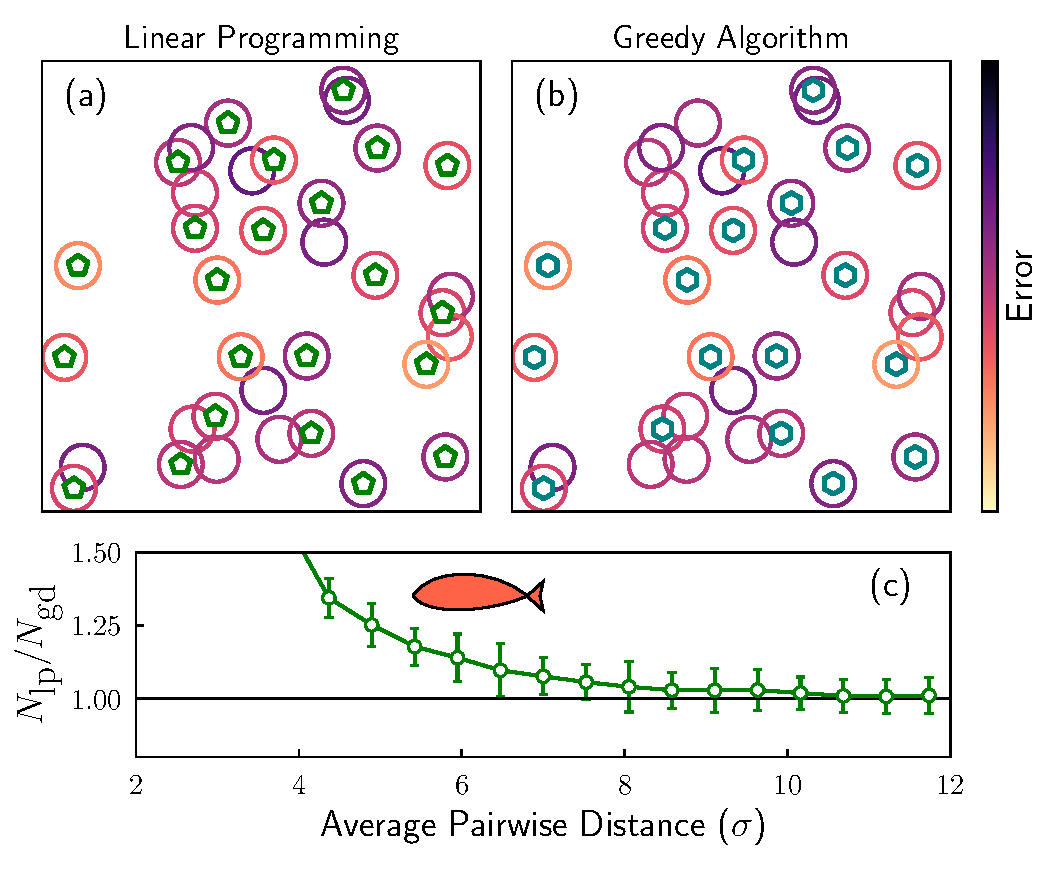
\includegraphics[width=\linewidth]{overlap}
  \caption[Removing the overlap particles with different algorithms]{
  The removal of overlapping particles with different algorithms. The circles represent particles. Their locations corresponds to $\{\mathbf{x}\}$, and their radius values are the hard core diameters ($\sigma$ in Eq.~\ref{eq:overlap}). The colour of the circles represents the error to be minimised.
  (a): the result of solving Eq.~\ref{eq:overlap}, implemented as algorithm~\ref{alg:overlap}. The pentagons represent the optimised result ($\{ \mathbf{x} \}_\textrm{opt}$).  
  (b): the result of greedy algorithm (algorithm~\ref{alg:overlap-greedy}). The hexagons represent the optimised result ($\{ \mathbf{x} \}_\textrm{opt}$).
  (c): the number ratio of optimised positions from algorithms~\ref{alg:overlap} ($N_\mathrm{lp}$) and algorithm~\ref{alg:overlap-greedy} ($N_\mathrm{gd}$) as a function of average pairwise. The positions were randomly sampled with different densities. The error bars were the standard error calculated from 25 different simulations.
  }
  \label{fig:overlap}
\end{SCfigure}


The systematic difference between the two algorithms is presented in Fig.~\ref{fig:overlap}(c). The ratio between the number of optimised particles, detected by different algorithms is plotted against the average pairwise distance of the particles. The linear programming method consistently generates larger optimised set, especially in the high density region, when the average pairwise distance is close to 2.
For the dilute system, the difference between the two algorithms were negligible. The average pairwise distance of zebrafish were close to 20 cm\cite{yang2021pcb,miller2007}, while the average body length of the fish was $\sim$ 3 cm. As a result, the fish is similar to the ideal gas particles where the average pairwise distance is close to 6 $\sigma$, where the difference between the two algorithms is significant. Because of its better performance, the linear programming method was selected to remove the overlapping particles. In the experiments, the size of the hard core was chosen to be 1 cm, a value that corresponds to the width of the fish.


\subsection{Removing Overlapping and \emph{Soft} Particles}

The overlap removing algorithm can be improved slightly, to change the strictly hard length scale ($\sigma$) to a ``softer'' counterpart. The idea was borrow from the soft margin classification problem for the support vector machine (SVM) algorithm in the machine learning (ML) community \cite{geron2019}. Following the naming tradition in ML literatures, we introduce a \emph{slack variable} $\zeta_{ij}$ for particle $i$ and $j$. The value of $\zeta_{ij}$ measures how soft the repelling is between two particles. The larger $\zeta_{ij}$ value corresponds to a softer particle. In the language of physics, the $\zeta_{ij}$ variables are essentially the pairwise potential energy between atoms, whose sum ($\sum_i\sum_j\zeta_{ij}$) gives the internal energy of a system, and should be minimised.

Formally, the overlap removing with soft interaction can be written down as follows,

\begin{equation}
\begin{aligned}
	\textrm{Minimize} && 
	\sum_i{(e_i + \mu) x_i} + \beta \sum_i \sum_j \zeta_{ij} \\
	\textrm{Subject to} &&  x_1 d_{12}  x_2 \le \sigma - \zeta_{12}\\
	&&  x_1 d_{13}  x_3 \le \sigma - \zeta_{13}\\
	&& \vdots  \\
	&& x_i d_{ij}  x_j \le \sigma - \zeta_{ij}
\label{eq:overlap-soft}
\end{aligned}
\end{equation}

\noindent which is a slight modification of Eq.~\ref{eq:overlap}.
Firstly, we remove the constraint that forces the total number of particles to equal $K$. 
There are also two additional parameters, \gls{mu} and \gls{beta}.
The parameter $\mu$ controls the number of total particles in $\{\mathbf{x}\}_\mathrm{opt}$. The smaller the $\mu$ value is, the more particles will be included in the optimised set. In the context of statistical mechanics, we can think of $\mu$ as the \emph{chemical potential}.
The parameter $\beta$ before the energy term $\sum_i\sum_j \zeta_{ij}$ controls the softness of the excluding zone around each coordinate, sharing the same meaning with the hyperparameter $C$ in the SVM algorithm. Within the context of statistical physics, the parameter $\beta$ is conceptually identical to the \emph{inverse temperature}. Reducing the value of $\beta$, we increase the temperature, and we make every particle appear softer. 

The solution of Eq.~\ref{eq:overlap-soft} will be identical to the solution of Eq.~\ref{eq:overlap}, when $\beta \rightarrow \infty$ and $\mu \sim -\max(\{ e_i \})$. These solutions were ascribed to the ``hard removal'' region in Fig.~\ref{fig:overlap-soft}(c). Fixing the value of $\mu$ but decrease $\beta$ gradually, move overlap will be allowed, and more particles will be detected. These regions were labelled as ``soft removal'' in Fig.~\ref{fig:overlap-soft}. When the values of both $\mu$ and $\beta$ were small, all the particles will be retained in $\{\mathbf{x}_\mathrm{opt}\}$, corresponding to the ``no removal'' region in Fig.~\ref{fig:overlap-soft}(c). On the other hand, the solution of Eq.~\ref{eq:overlap-soft} will lead to the removal of all particles, when the value of $\mu$ is large. This scenario corresponds to the ``excess removal'' region in Fig.~\ref{fig:overlap-soft}(c).


\begin{SCfigure}
  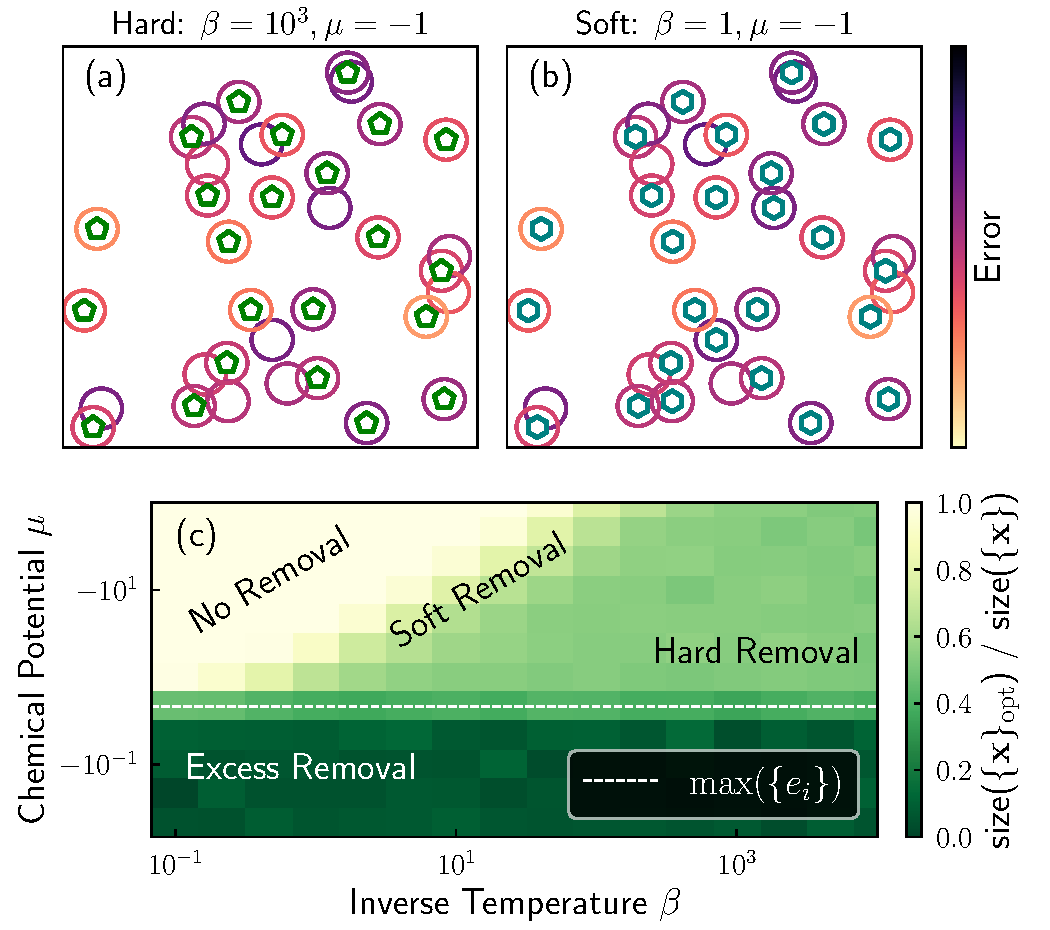
\includegraphics[width=\linewidth]{overlap-soft}
  \caption[Removing the overlap particles with soft constraint]{
  The removal of overlapping particles following equation~\ref{eq:overlap-soft}. The circles represent particles ($\{\mathbf{x}\}$). The colour of the circles represent their errors.
  (a): the result with parameters $\beta=10^3$ and $\mu=-1$. The pentagons represent the optimised result ($\{ \mathbf{x} \}_\textrm{opt}$). The result is identical to that in Fig.~\ref{fig:overlap}.
  (b): the result with parameters $\beta=1$ and $\mu=-1$. The pentagons represent the optimised result ($\{ \mathbf{x} \}_\textrm{opt}$).
  (c): the ratio between the number of particles after and before the optimisation, as a function of the two parameters. The $x$ axis corresponds to the inverse temperature $\beta$, and the $y$ axis corresponds to the chemical potential $\mu$. Different regions were labelled with their characteristic behaviour. The dashed line shows the maximum value of the error. Each grid in (c) represents the average of 25 ideal-gas simulations.
  }
  \label{fig:overlap-soft}
\end{SCfigure}


This soft overlap-removal algorithm was implemented, but not tested nor used for the fish data. This is because the determination of the parameters, $\mu$ and $\beta$, is difficult. However, this soft overlap remove algorithm presents as a promising algorithm for the real-space colloidal microscopy, as the energy term can take realistic, inter-colloidal interaction form, to match the experimental system.

\section{From Better Locations to Trajectories}
\label{section:link}

The overlap-free positions can be linked into trajectories, from which we can get the velocities of the fish. The term ``link'' means finding the fish $j$ at time $t+1$, which corresponds to the fish $i$ at time $t$, and the pair $(i, j)$ forms a link.
Such a linking process therefore gives us the identity of each fish in different time points.
The movement of a single fish, as a function of time, forms a \emph{trajectory}.
The process of linking coordinates into trajectories is commonly applied in different fields, for instance in the analysis of colloidal experiments\cite{crocker1996} as well as fluid dynamic experiments\cite{ouellette2005ef}.


Two examples of the linking process are illustrated in Fig.~\ref{fig:link-idea}, where the locations of 6 simulated fish in 3 successive frames were linked into 6 trajectories. The good links were illustrated in Fig.~\ref{fig:link-idea}(a) while the poor links were shown in Fig.~\ref{fig:link-idea}(b).
Visually, the trajectories in (b) were poor because the resulting trajectories contain sudden jumps between different locations. Intuitively, we would not expect the fish to jump back and forth from place to place.

The method of linking experimental coordinates of animals into trajectories always involves some ``educated guesses''. This is because we do not know the underline dynamics of the animals that we were studying, as we could not predict precisely where the animal will move to from its past trajectory. In this section, two heuristic methods that ``worked'' will be introduced.


\subsection{Equilibrium Linking}
\label{section:link-eq}


With the observation in Fig.~\ref{fig:link-idea}, it is reasonable to assume that the links yielding smallest total movement for all the fish, are good links. Formally, our linking procedure will aim at minimising the total squared movement \gls{tsm}, which is written as 

$$
\Delta = \sum_i\sum_t\delta_i(t)^2,
$$

\noindent where $i$ corresponds to all the linked trajectories, and $\delta_i(t)$ is the distance that a fish travelled between time $t-1$ and $t$. In fact, \citeauthor{crocker1996} showed that the minimisation of $\Delta$ is equivalent to maximising the probability, if the fish were non-interacting diffusive Brownian particles in equilibrium \cite{crocker1996}.
Even though the underlying assumption is crude, this method produces visually good trajectories for fish.
The linking algorithm that minimises $\Delta$ is termed as \emph{equilibrium linking}, since it is suitable for physical systems in equilibrium.


\begin{SCfigure}
  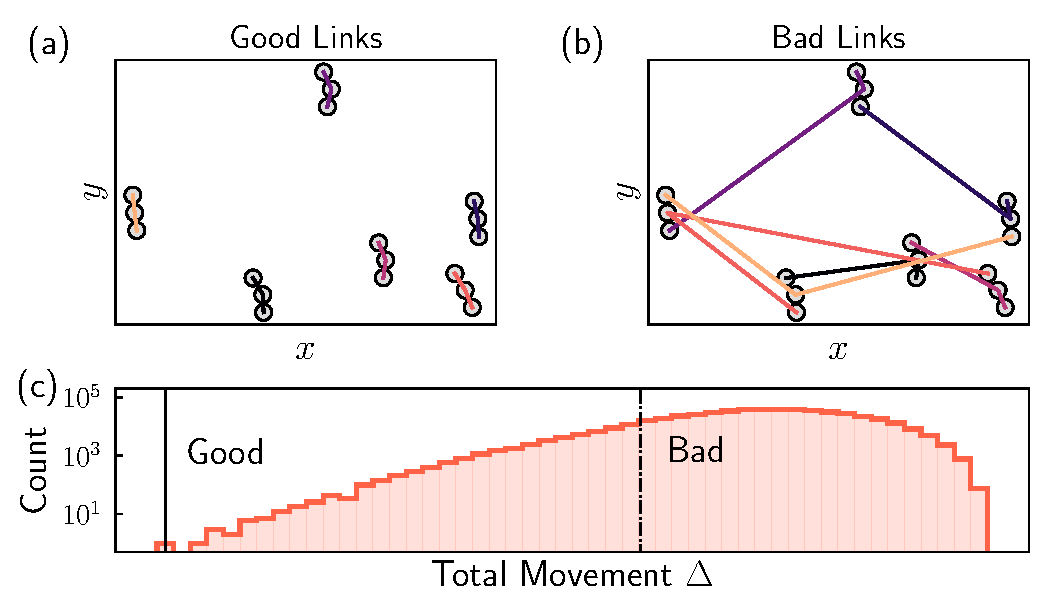
\includegraphics[width=\linewidth]{linking-idea}
  \caption[Linking locations into trajectories: concept illustration]{
  (a): the good way to link positions in 3 successive frames into trajectories.
  (b): the bad way to link positions in 3 successive frames into trajectories.
  (c): The distribution of total movement ($\Delta$) for all the possible linking options ($6!^2=518,400$ possibilities). The good linking result corresponds to the links that yields the minimum of $\Delta$.
  }
  \label{fig:link-idea}
\end{SCfigure}


Unfortunately, the minimisation of \gls{tsm} is a difficult task. Naively, we may attempt to list all the possible links, and choose the one with minimum $\Delta$ value as our linking result. However, the complexity of this approach is $\mathcal{O}((N!)^{T-1})$ \cite{crocker1996}, where $N$ is the number of fish, and $T$ is the total number of time points. For the experiment with 10 fish in 20 total frames, we need to enumerate $\sim 10^{130}$ possible combinations, which is not practical.\marginfootnote{
	To find the minimum number in an array with size of $10^{130}$, we need $\sim 10^{103}$ years, using a laptop with infinite memory. People die in the timescale of $\sim 10^2$ years.
}

To reduce the complexity, we restrain the particles to have a maximum movement between two frames \cite{crocker1996}, and analyse the data frame-by-frame, rather than optimise the entire trajectory. A good implementation of this approach is available in the \code{Trackpy} package \cite{allan2021}. Unavoidably, the introduction of extra assumptions will deviate the obtained solution, the linked trajectories, away from the true global minimum of $\Delta$. And even with the reduced complexity, the equilibrium linking algorithm can be extremely slow, when multiple equally good linking options being available.

\subsection{Active Linking}
\label{section:link-act}

\begin{SCfigure}
  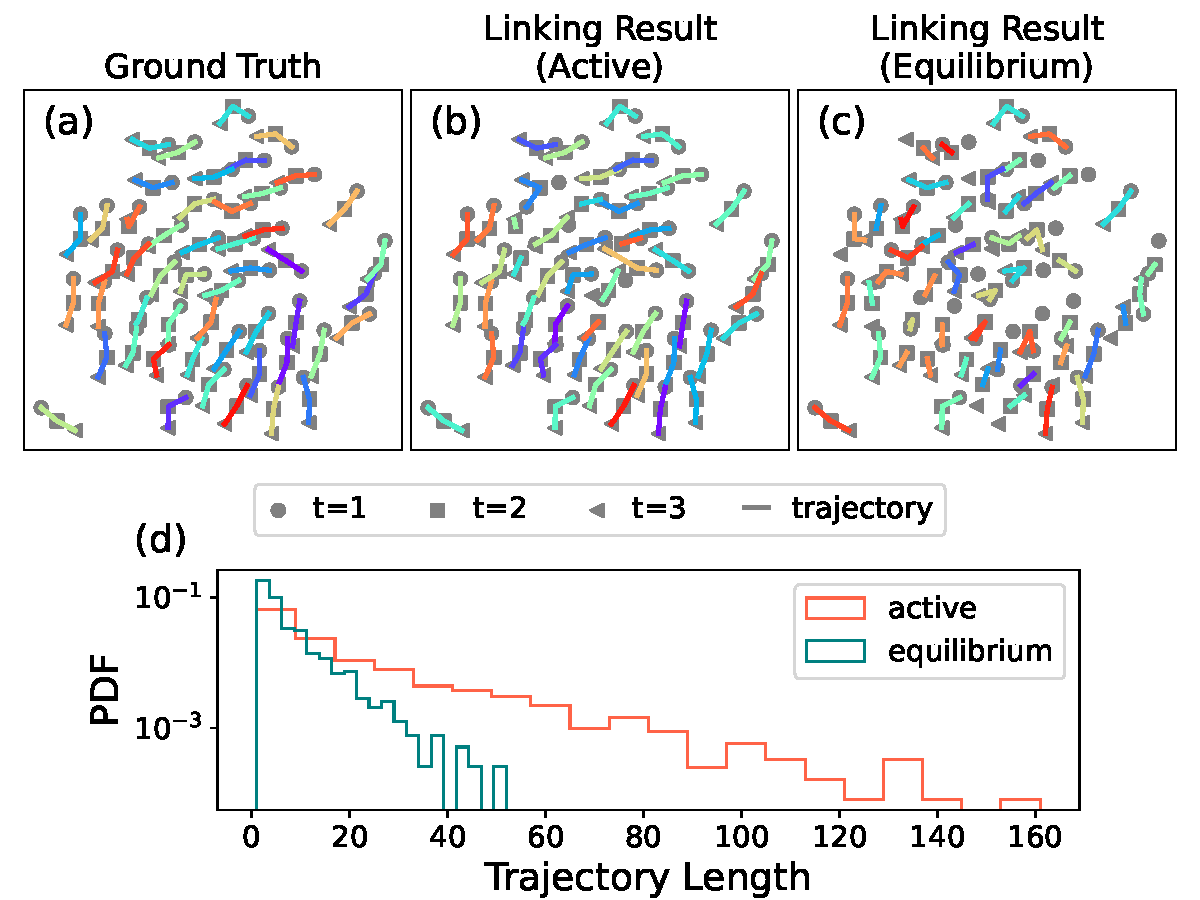
\includegraphics[width=\linewidth]{linking-sim}
  \caption[Comparing two linking algorithms]{
  The linking process to get trajectories from positions. The grey solid scatters represents the location ($\{\mathbf{x}\}$) of simulated particles. The coloured lines represent the linked trajectories. Some positions were discarded (rendered as empty scatters) randomly to mimic the experimental locations.
  Left: the ground truth.
  Middle: the result with the active linking algorithm.
  Right: the result with the equilibrium linking algorithm.
  }
  \label{fig:link-sim}
\end{SCfigure}

For systems that are out of equilibrium, like a school of fish, the assumption introduced in section~\ref{section:link-eq} is not formally correct. In this project, another good heuristic approach proposed by \citeauthor{ouellette2005ef} was used to link the coordinates \cite{ouellette2005ef}.
For particle $i$ at time $t$ and particle $j$ at time $t+1$, the link $(i, j)$ was established by minimising the \emph{tracking cost},

$$
\phi_{ij}^{t} = \left\Vert
\mathbf{x}_j^{t+2} - \hat{\mathbf{x}}_i^{t+2}
\right\Vert,
$$

\noindent where $\mathbf{x}_j^{t+2}$ is the location of particle $j$ in time point $t + 2$, and $\hat{\mathbf{x}}_i^{t+2}$ is the predicted location of particle $i$ in time point $t + 2$. The prediction was calculated with the following

$$
\begin{aligned}
\hat{\mathbf{x}}_i^{t + 2} &= 
\mathbf{x}_i^t + 
\mathbf{v}_i^t + 
2 \mathbf{a}_i^t = 
3 \mathbf{x}_i^{t+1} - 
3 \mathbf{x}_i^t +
\mathbf{x}_i^{t-1} \\
\mathbf{v}_i^t &= (\mathbf{x}_i^{t+1} - \mathbf{x}_i^{t - 1}) / 2 \\
\mathbf{a}_i^t &= 
\mathbf{x}_i^{t+1} - 2 \mathbf{x}_i^{t} + \mathbf{x}_i^{t-1}.
\end{aligned}
$$

\noindent In reference~\cite{ouellette2005ef} this method was named as the four frame best estimate method. Operationally, for particle $i$ in time point $t$, we search for all the possible particle $j$ in time point $t+1$, and establish link with the minimum $\phi_{ij}^t$, by predicting the location of the trajectory with link $(i, j)$ in time point $t + 2$. This linking method is noted as the \emph{active} linking method.

The behaviour of the two linking methods was exhibited in Fig.~\ref{fig:link-sim}, where simulated trajectories were used for the test. The model used in the simulation is the inertial Vicsek model, which will be introduced in chapter~\ref{chapter:fish_model}. The model generates trajectories that are similar to that of the zebrafish, and the generated coordinates were used to test the different linking algorithm.
Both methods generated visually good trajectories.
However, the equilibrium linking method obtain shorter trajectories, as shown in Fig.~\ref{fig:link-sim}, which indicates that the behaviour of the equilibrium linking method is poor. For all the fish data, the active linking method was used.



\subsection{Extending the Trajectories}

The linking algorithms typically give us some short trajectory segments. These segments can be extended further following \citeauthor{xu2008}'s method. The idea is to join the two trajectories together, if the the prediction from earlier trajectory matched the locations of the later trajectory \cite{xu2008}.

The result of the relinking method is illustrated in Fig.~\ref{fig:relink}. The coordinates to be linked and relinked was generated from simulation, where 25 simulated agents were performing a U-turn together. Some of the coordinates (2\%) were deliberately removed during linking, in order to mimic the various locating errors in reality. 

For perfect coordinates, the active linking method was capable of obtaining correct trajectories. However, the introduction of missing particles makes this linking process problematic. As illustrated in Fig.~\ref{fig:relink}(a), many short trajectory segments were obtained. The relinking process successfully re-joined these segments into very long trajectories, as shown in Fig.~\ref{fig:relink}(b). The relinked trajectories were very long, and half of them have the full length, as shown in Fig.~\ref{fig:relink}(c). For the experimental fish coordinates, the relinking process is valuable, as it always extends the short trajectories (from the active linking method) into longer ones.


\begin{SCfigure}
  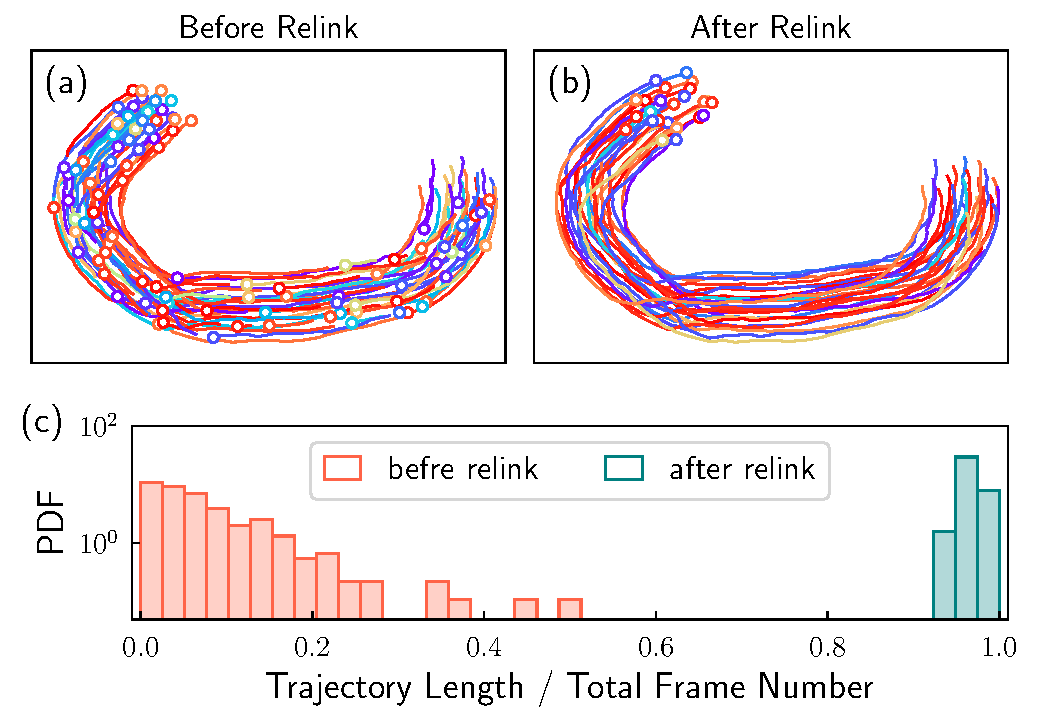
\includegraphics[width=\linewidth]{relink}
  \caption[The effect of relinking]{
  	The effect of relinking process with simulated data.
  	(a) The trajectories linked with the active linking method.
  	(b) The trajectories extended with the relinking method.
  	(c) The distribution of the trajectory length. The length values were rescaled by the total frame number. The trajectory with length value being close to 1 corresponds to a full trajectory through out the entire simulation.
  }
  \label{fig:relink}
\end{SCfigure}


\section{From Trajectories to Behaviour}
\label{section:trajectory-analysis}

The trajectories contain rich information about the behaviour of the zebrafish.
The analysis to reveal the behaviour of the fish will be discussed in this section.
For the structure of the fish group, we introduce the nearest neighbour distance, the convex hull, and the radial distribution function, as different characterisation tools. On the other hand, the average speed, the orientational relaxation time, the polarisation order and the persistence length will be discussed as the quantities to describe the dynamics of the fish.


\subsection{The Structure}

The coordinates of the fish shed light on the the \emph{structure} of the group, giving answers to the following questions.

\begin{enumerate}
	\item How close do a pair of fish stay to each other?
	\item How big is the animal group in terms of the metric size?
	\item Are the fish arranged in an ordered way (like atoms in a crystal) or a disordered way (like atoms in a fluid phase)?
\end{enumerate}

To answer the first question, we can calculate the nearest neighbour distance of the fish, whose usage could be traced back to 1960s \cite{cullen1965}. The average nearest neighbour distance of fish (\gls{lnn}) is defined as,

\begin{equation}
	l_\textrm{nn} =\frac{1}{N}\sum_i\min_{j (\neq i)}(d_{ij})
\label{eq:nnd}
\end{equation}

\noindent where \gls{dij} is the pairwise distance of fish $i$ and $j$, and $N$ is the total amount of fish. The average nearest neighbour distance of a group could serve as a measure of the cohesiveness of the fish. The group with smaller $l_\textrm{nn}$ value appear more cohesive.

To measure the size of the group, we can measure area (for 2D data) or the volume (for 3D data) of the \emph{convex hull}, constructed from the coordinates of the fish. The convex hull is the smallest subset of the space, which contains all line segments connected by all pairs of points \cite{berg2000}. Intuitively, the convex hull is the smallest polygon (or polyhedron for 3D coordinates) that encloses all coordinates. An example of the convex hull constructed from 50 fish were provided in Fig.~\ref{fig:structure-2d}(a). The area ($A_\mathrm{ch}$) or the volume ($V_\mathrm{ch}$) of the hull can be transformed into a lengthscale, termed as the \emph{effective convex hull diameter} \gls{lch}, which is defined as

\begin{equation}
\begin{split}
	l_\mathrm{ch}
	&= \left(
	\frac{4}{\pi} A_\mathrm{ch}
	\right)^\frac12 (\mathrm{2D}\ \mathrm{Coordinates}) \\[1.5ex]
	&= \left(
	\frac{6}{\pi} V_\mathrm{ch}
	\right)^\frac13 (\mathrm{3D}\ \mathrm{Coordinates}),
\end{split}
\label{eq:convex-hull-diameter}
\end{equation}

\noindent where the shape of the convex hull were assumed to be circular (for 2D coordinates) or spherical (for 3D coordinates). The effective convex hull diameter is a measure of the group size.

Both lengthscales, the effective convex hull diameter and the nearest neighbour distance, capture the cohesiveness of the group. In fact, they were often linearly correlated for the zebrafish, as shown in Fig.~\ref{fig:nnd-ch-corr}. Therefore, we only need one of them to describe the fish behaviour. The nearest neighbour distance was selected, because it is more widely used in the past.

\marginpar{
\centering
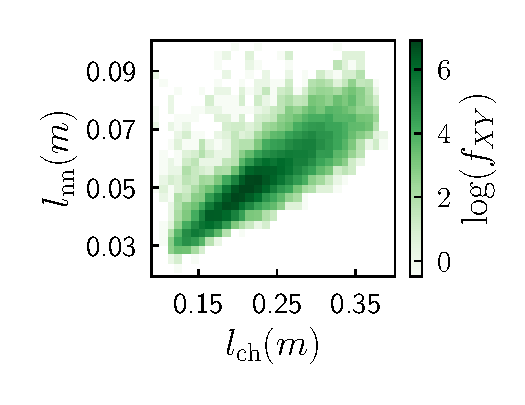
\includegraphics[width=\marginparwidth]{nnd-ch-corr}
\captionof{figure}{The joint probability density function ($f_{XY}$) of $l_\mathrm{nn}$ and $l_\mathrm{ch}$. The results were obtained from 3D experimental data of 50 adult zebrafish.}
\label{fig:nnd-ch-corr}
}


Finally, we can calculate the radial distribution function (the $g(r)$) of the fish to inspect whether the structure of the fish was ordered or not. However, the spatial distribution of a group of fish may not be homogeneous in the experiment, possibly being affected by environmental factors such as the distribution of brightness, as shown in the results in chapters~\ref{chapter:fish_2d} and \ref{chapter:fish_3d}. Therefore, the pairwise distances ($\{ d_{ij} \}$) would be biased to favour the lengthscale of the high density region. In other words, the fish appear to swim together. But they were driven by an external field, instead of being attractive to each other.

To remedy the effect of the external field, we can compare the pairwise distances of the fish $\{d_{ij}\}^\textrm{fish}$ to the pairwise distances of the ideal gas particles $\{d_{ij}\}^\textrm{gas}$, that share the same inhomogeneous spatial distribution with the fish.
Operationally, we calculate the density distribution of the fish, and sample ideal gas particles drawn randomly from the same density distribution, using the tower-sampling method \cite{krauth2006}.
Therefore, the sampling of the ideal gas particles is biased, in contrast to a uniform distribution in the boundary. The biased sampling result was illustrated in Fig.~\ref{fig:structure-2d}(a) and Fig.~\ref{fig:structure-3d}(a), where the distribution of the ideal gas is identical to that of the fish.


Even though the biased ideal gas particles share the same density distribution with the fish, these two systems are inherently different. The ideal gas particles do not interact with each other, but the fish do.
Such a difference will lead to different pairwise distances, whose probability density function was noted as \gls{pdfd}.
For instance, we can not imagine two fish with a separation of zero, as the fish can not physically overlap.
Such a repulsive interaction will decrease the likelihood of finding two fish at very short distances.
 
The ratio between the $f_d(r)$ from the fish and the ideal gas, was defined as the radial distribution function, \gls{gr}:

\begin{equation}
	g(r) = \frac{f_d^\textrm{fish}(r)}{f_d^\textrm{gas}(r)}.
\label{eq:gr}
\end{equation}

\noindent The value of $g(r)$ indicates the likelihood of finding a pair of fish at the distance $r$, with respect to the ideal gas particles. When $g(r)$ is equal to one, it is equally likely to find a pair of fish or to find a pair of ideal gas particles, indicating the lack of correlation. When the value of $g(r)$ is greater than one, the density of the fish correlates positively, suggesting a cohesive behaviour.

For the structure of dilute liquid, we often get a peak in the $g(r)$, followed by a monotonic decay. The location of the peak is often close the $l_\mathrm{nn}$. The subsequent decay revealed another lengthscale, which was termed the correlation length of the density ($\xi_\rho$). The definition of \gls{xirho} is

\begin{equation}
	g(\xi_\rho) = 1; (\xi_\rho > l_\mathrm{nn}).
\label{eq:length-density}
\end{equation}

\noindent and we force the value of $\xi_\rho$ to be greater than $l_\mathrm{nn}$, effectively removing the situation where $g(r)$ reaches zero at very small distance values.

In addition to the lengthscales, the height of the peak of $g(r)$ give us a measure of the cohesiveness of the group. Inspired by liquid state theory, we define the logarithm of the peak value of $g(r)$ as the \emph{effective attraction} \gls{attr} \cite{hansen2013}:

\begin{equation}
\epsilon = -\log\left(
	\max(g(r))
\right).
\label{eq:effective-attraction}
\end{equation}

\noindent The quantity $\epsilon$ is a better measure of the cohesion of the fish, because it could differentiate whether the fish is cohesive or not. For a non-cohesive group, the value of the $g(r)$ will be close to one, leading a value of 0 for $\epsilon$. The lack of cohesion could be be identified by the lengthscales.


\begin{table}
\begin{adjustwidth*}{0in}{-1.5in}
	\centering
	\begin{tabular}{ l l c c l }
		\toprule
		Symbol & Definition & Value (2D) & Value (3D) & Meaning\\
		\midrule
		$l_\mathrm{nn}$ &
		Eq.~\ref{eq:nnd} &
		61 $\pm$ 10 mm &
		51 $\pm$ 10 mm &
		Nearest Neighbour Distance
		\\
		$l_\mathrm{ch}$ &
		Eq.~\ref{eq:convex-hull-diameter} &
		0.8 $\pm$ 0.46 m &
		0.29 $\pm$ 0.25 m &
		Convex Hull Diameter\\
		$l_p$ &
		Eq.~\ref{eq:lp} &
		$\sim 0.13$ m &
		$\sim 0.14$ m &
		Persistence Length\\
		$\xi_\rho$ &
		Eq.~\ref{eq:length-density} &
		$\sim 0.4$ m &
		$\sim 0.32$ m &
		Correlation Length of the Density\\
		$\xi_v$ &
		Eq.~\ref{eq:length-dynamics} &
		$\sim 0.15$ m &
		$\sim 0.12$ m &
		Correlation Length of the Speed\\
		$\xi_\mathbf{o}$ &
		Eq.~\ref{eq:length-dynamics} &
		$\sim 0.38$ m &
		$\sim 0.24$ m &
		Correlation Length of the Orientation\\
		$\tau_\mathbf{o}$ &
		Eq.~\ref{eq:tau} &
		$\sim 1.3$ s &
		$\sim 0.9$ s &
		Relaxation Time of the Orientation\\
		$\tau_\rho$ &
		Eq.~\ref{eq:tau} &
		$\sim 900$ s &
		$\sim 180$ s &
		Relaxation Time of the Density\\
	\bottomrule
	\end{tabular}
\caption{
Different Length Scales and Time Scales for 50 Zebrafish.}
\label{table:behaviour}
\end{adjustwidth*}
\end{table}

\subsection{The Dynamics}

The velocities can be calculated as the time derivative of the positions along the trajectories, once we linked the coordinates. The velocities offered the \emph{dynamics} of the system, giving answers to the following questions.

\begin{enumerate}
	\item How fast do the fish swim?
	\item Is the movement of the fish ordered or random?
	\item How long does it take for the fish group to forget its current state?
\end{enumerate}

To answer the first question, we could simple calculate the average speed of the fish, which is defined as,

\begin{equation}
	v = \frac1N \sum_i{\left\Vert \mathbf{v}_i \right\Vert},
\label{eq:speed}
\end{equation}

\noindent where the $\mathbf{v}_i$ is the location of fish $i$, and $N$ is the total amount of the fish. With higher \gls{spd} value, the animals on average move faster.
The distribution of the average speed of 50 zebrafish in 3D was shown in Fig.~\ref{fig:dynamics-3d}(a).

Being conceptually similar to the average speed, the speed of the entire group can be calculated as,

$$
v_g = \frac1N \left\Vert
\; \sum_i{\mathbf{v}_i} \;
\right\Vert.
$$

\noindent This quantity indicates the speed of the group centre. A large group speed value indicates the fish  moving collectively from one place to another. Formally, we define an \emph{order parameter} to describe such behaviour, by modifying the group speed:

\begin{equation}
	\Phi = \frac1N \left\Vert
		\; \sum_i \mathbf{o}_i \;
	\right\Vert
	= \frac1N \left\Vert
		\sum_i \frac{\mathbf{v}_i}{\Vert \mathbf{v}_i \Vert}
	\right\Vert,
\label{eq:polarisation}
\end{equation}

\noindent where \gls{pol} is called the \emph{polarisation}\marginfootnote{
	The polarisation is conceptually similar to the magnetisation per spin in the Ising model. When the order parameter approaches one, the system is ordered.
	The polarisation is identical to the magnetisation defined in XY model (in 2D) and Heisenberg model (in 3D), when the orientations of the fish was treated as the spin vectors \cite{newman1999}.
}, and $\mathbf{o}_i$ is the orientation of fish $i$. The definition of $\Phi$ ensures it varies from 0 to 1, like other order parameters in statistical mechanics.
The movement of a group of fish is ordered if the value of $\Phi \sim 1$, and the movement being disordered when $\Phi \sim 0$.


For a group of fish, their structural quantities ($l_\mathrm{nn}, l_\mathrm{ch}, g(r)$) and their dynamic quantities ($v, \Phi$) change constantly. With the \emph{time-displaced autocorrelation function} (ACF) of these quantities, we can probe the typical timescale for the fluctuation of these quantities. The ACF of quantity \gls{cat} is defined as, \cite{newman1999}

\begin{equation}
\begin{split}
	C_\mathcal{A}(t)
	&= \int d\tau
	\left(
		\mathcal{A}(\tau) - \bar{\mathcal{A}}
	\right)
	\left(
		\mathcal{A}(\tau + t) - \bar{\mathcal{A}}
	\right) \\
	&= \langle \mathcal{A}(t) \mathcal{A}(t + \tau) \rangle.
\label{eq:acf}
\end{split}
\end{equation}

\noindent where $\bar{\mathcal{A}}$ is the time-average $\mathcal{A}$. For the ACF of the orientation of the fish, the shape of \gls{cot} exhibits a typical exponential decay. Such ACF was commonly obtained from the Markov processes, where the $C_\mathcal{A}(t)$ could be written as a sum of exponential functions,

\begin{equation}
\begin{split}
	C_\mathcal{A}(t) &= \sum_i \left( a_i \exp{-t / \tau_i} \right)\\
	&\sim \exp\left(-t / \tau\right).
\end{split}
\label{eq:tau}
\end{equation}

\noindent Here the shape of $C_\mathcal{A}$ is often dominated by the largest time scale ($\tau$).\marginfootnote{
This timescale corresponds to the second largest eigenvector of the transition matrix of the Markov process.
}
Therefore, we define the timescale when $C_\mathbf{o}$ reaches $1/e$ as the relaxation time orientation, noted as $\tau_\mathbf{o}$. For other quantities, the shapes of their corresponding $C_\mathcal{A}(t)$ functions are complicated. We therefore define the time when their corresponding $C_\mathcal{A}(t)$ reach zero as their relaxation time scales.

Regardless of the slightly different definition, the value of the relaxation time \gls{taua} indicates the time taken for a system to forget its current state.
For instance, the value of $\tau_\mathrm{nn}$ is the time for a group fish to forget their nearest neighbour distance. Because the two density-related quantities, $l_\mathrm{nn}$ and $l_\mathrm{ch}$, are strongly correlated, their corresponding ACFs ($C_\mathrm{nn}(t)$ and $C_\mathrm{ch}(t)$) are also very similar. Therefore, we term their relaxation time as the relaxation time of density, written as $\tau_\rho$. The examples of relaxation time scales for the orientation and density are available in Table~\ref{table:behaviour}. Practically, these two time scales are the only dominating time scales for the fish, in all of our observations.


In addition to the timescale of the structural quantities, we could also calculate the lengthscale of the dynamical quantities. For instance, we can take the the product of the average speed $v$ (Eq.~\ref{eq:speed}) and the orientation relaxation time $\tau_\mathbf{o}$ (Eq.~\ref{eq:tau}), as the \emph{persistence length}:

\begin{equation}
	l_p = v \ \tau_\mathbf{o}.
\label{eq:lp}
\end{equation}

\noindent The value of \gls{lp} corresponds to the distance that a fish travels in a straight fashion. For the fish with a small $l_p$ value, its trajectory appear more curvy. 

In addition to the persistence length, we can also measure the correlation length of the dynamics of the fish. If a fish changed its speed at a certain time point, it is interesting to know how far would such change reach. To do so, we calculate the \emph{connected correlation function} of the dynamical quantities \cite{newman1999, cavagna2014}\marginfootnote{
	The correlation function $C_\mathcal{A}(r)$ with variable ``$r$'' is a spatial correlation function, which gives us a correlation length $\xi_\mathcal{A}$. The correlation function $C_\mathcal{A}(t)$ with variable ``$t$'' is a temporal correlation function, which gives us a relaxation time $\tau_\mathcal{A}$.
}:

\begin{equation}
\begin{split}
	C_{\mathcal{A}}(r) 
	&= \iint d\mathbf{r} d\mathbf{r^\prime} \;
	\left(
		\mathcal{A}(\mathbf{r}) - \bar{\mathcal{A}}
	\right)
	\left(
		\mathcal{A}(\mathbf{r} + \mathbf{r^\prime}) - \bar{\mathcal{A}}
	\right)
	\delta(\Vert \mathbf{r} - \mathbf{r^\prime} \Vert - r) \\[2ex]
	&= \frac{\sum_i\sum_{j \neq i}
		\left[
			(\mathcal{A}_i - \bar{\mathcal{A}})
			(\mathcal{A}_j - \bar{\mathcal{A}})
			\delta(r - r_{ij})
		\right]
	}
	{\sum_i\sum_{j \neq i} \delta(r - r_{ij})}
\label{eq:cr}
\end{split}
\end{equation}

\noindent where $\delta(r - r_{ij}) = 1$ when $r = r_{ij}$, and it equals zeros otherwise. The correlation functions often exhibits a monotonic decay when $r > l_\mathrm{nn}$. We define the length when the correlation function $C_\mathcal{A}(r)$ reaches zero as the \emph{correlation length} of $\mathcal{A}$:

\begin{equation}
	C_{\mathcal{A}}(\xi_\mathcal{A}) = 0.
\label{eq:length-dynamics}
\end{equation}


\noindent The examples of the correlation functions for the speed \gls{cvr} and for the orientation \gls{cor} were shown in Fig.~\ref{fig:dynamics-2d}(e) and Fig.~\ref{fig:dynamics-3d}(e).

%Figure~\ref{fig:dynamics} (e) shows the correlation function for the orientation ($C_\mathbf{o}(r)$) and the speed ($C_{v}(r)$) from 50 zebrafish. It is obvious that these quantities exhibits different length-scales.

%Then we obtain $l_\mathbf{o} \sim 0.2m$, and $l_v \sim 0.1 m$. This indicates that the orientation of the fish would affect neighbours further away, than the speed of the fish. This might be the reason that the fish do not form a coherent, flocking group like the birds, as they do not synchronise their speed effectively. In addition, the correlation length of the orientation, $l_\mathbf{o}$, is smaller than the effective convex hull diameter ($l_\mathrm{cm}$) of the fish. This is similar to the correlation length of midges in the laboratory \cite{vandervaart2020}.



\section{The Behaviour of 50 Zebrafish in 2D}

The coordinates of 50 zebrafish in a quasi-2D experiment, obtained with the methods introduced in chapter~\ref{chapter:fish_2d}, were linked into trajectories, from which the behaviour of these fish were analysed.

\subsection{The Structure}
\label{section:analysis-structure-2d}


The structure of 50 zebrafish was shown in Fig.~\ref{fig:structure-2d}. The spatial distribution was presented in Fig.~\ref{fig:structure-2d}(a), which was used to sample the biased ideal gas particles. The distribution of the pairwise distance, $f_d(r)$, was presented in Fig.~\ref{fig:structure-2d}(b). It is obvious the fish were more cohesive than the ideal gas particles, indicated by the mode of the distribution of the pairwise distances. The ratio of these distributions gives the $g(r)$ of the fish (Eq.~\ref{eq:gr}), which is shown in Fig~\ref{fig:structure-2d} (c). The distribution of $l_\mathrm{nn}$ and $l_\mathrm{ch}$ are presented in Fig~\ref{fig:structure-2d} (d).

The important structural feature revealed in Fig~\ref{fig:structure-2d} is the separation of $\xi_\rho$ and $l_\mathrm{ch}$, as the effective convex hull diameter ($l_\mathrm{ch}$, Eq.~\ref{eq:convex-hull-diameter}) is much larger than the correlation length of the density ($\xi_\rho$, Eq.~\ref{eq:length-density}).
This corresponds to the fragmentation of the fish group, where the 50 fish separated into sub-clusters. This scenario was plotted in Fig.~\ref{fig:structure-2d}(a), where the locations of the fish were represented as cross markers. There are clearly two dense blobs within the convex hull. And the size of these dense blobs is accurately captured by $\xi_\rho$.

As a consequence of the monotonic decay in $g(r)$, the fish group present a void at larger separation distances, where the value of $g(r) < 1$, shown in Fig.~\ref{fig:structure-2d}(a). As a result of the fragmentation of the fish group, the void also appear inside the fish group. The fragmentation of the fish group could explain the very wide distribution of $l_\mathrm{ch}$ observed in Fig.~\ref{fig:structure-2d}(d). If two sub-groups meet, the entire group will have a small value for its $l_\mathrm{ch}$. If the sub-groups were separated, the fish will exhibit a large $l_\mathrm{ch}$ value. 


 \begin{SCfigure}
  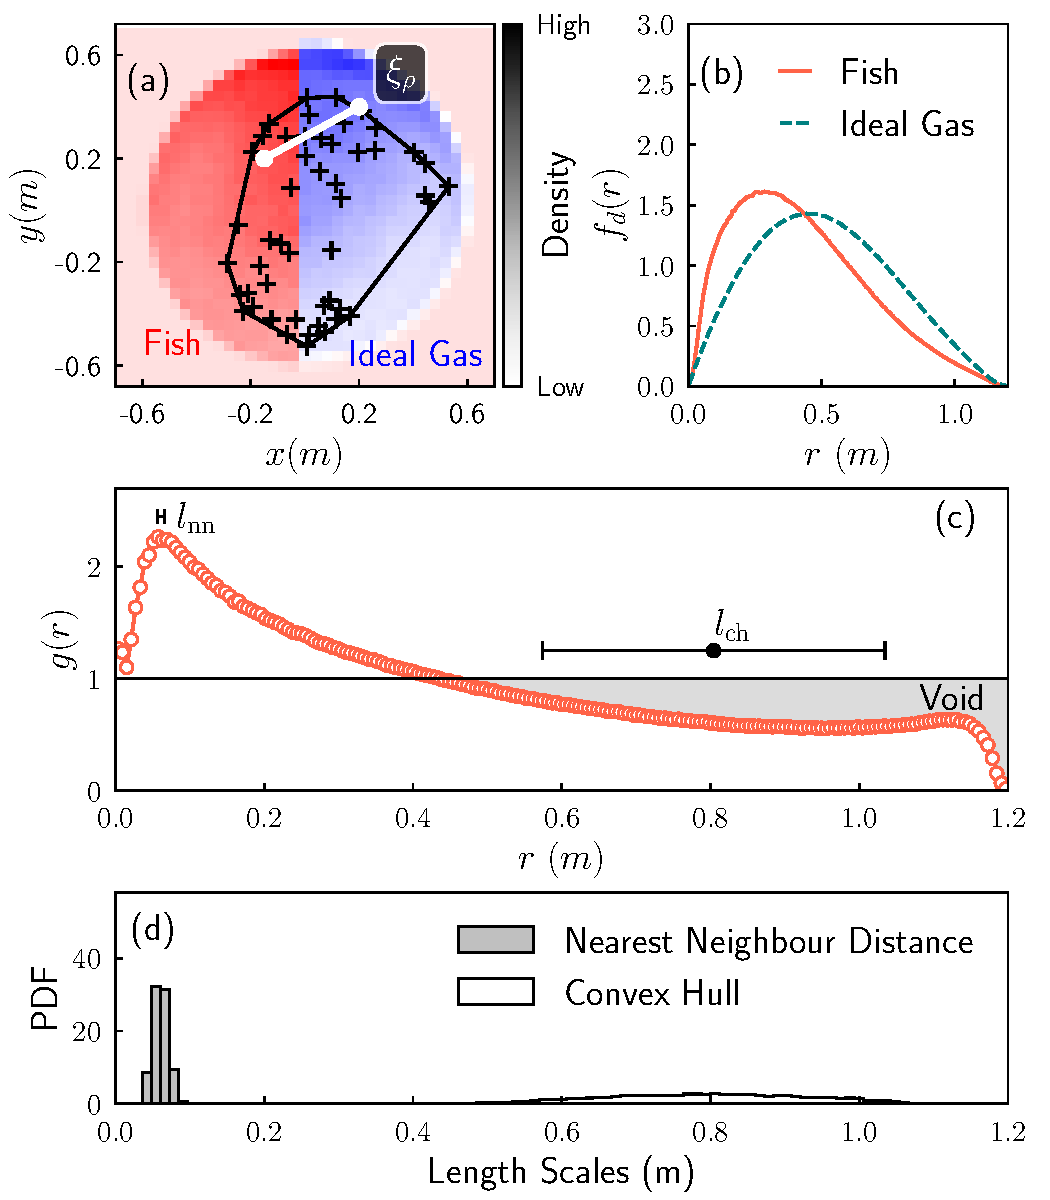
\includegraphics[width=\linewidth]{structure-2d-50}
  \caption[The structure of 50 zebrafish in 2D]{
  The structure of 50 zebrafish in a quasi-2D experiment.
  	(a) The joint distribution of the $x$ and $y$ coordinates of the fish and the ideal gas particles. The distribution of the ideal gas were biased to be identical to the fish. The location of 50 fish at one time point were plotted as circles. The boundary convex hull of these 50 scatters were plotted as solid lines.
  	(b) The probability density function of the pairwise distributions for the fish and the ideal gas particles in 2D.
  	(c) The radial distribution function, $g(r)$ (Eq.~\ref{eq:gr}) of the fish. It is defined as the ratio between the two PDFs in (b). Two important length scales, the nearest neighbour distance and the size of the convex hull were captured by the $g(r)$. The long distance region where $g(r) < 1$ corresponds to the void in the tank, where the group were able to explore.
  	(d) The distribution of the nearest neighbour distance and the effective diameter of the convex hull, of the fish.
  }
  \label{fig:structure-2d}
\end{SCfigure}

\subsection{The Dynamics}

The dynamics of the 50 fish are shown in Fig.~\ref{fig:dynamics-2d}. Figure~\ref{fig:dynamics-2d} (a) - (c) shows the distribution of the polarisation $\Phi$ (Eq.~\ref{eq:polarisation}) and the average speed $v$ (Eq.~\ref{eq:speed}). Their joint distribution appear to be very weakly correlated, as exhibited in Fig.~\ref{fig:dynamics-2d}(b). Overall, the fish were in a random state where $\Phi \sim 0.25$.



The ACFs (Eq.~\ref{eq:acf}) of different quantities were shown in Fig.~\ref{fig:dynamics-2d}(d). Two well separated time scales could be identified from these functions. For the time scale of $\sim$ 1s, the fish changed its orientation, and the value of $C_\mathbf{o}(t)$ decays to $1/e$. This timescale also dominates the ACF of the polarisation ($C_\Phi(t)$). 

Ones possible explanation for this observation, is to assign an intrinsic orientational diffusion constant for the fish. In other words, we assume the fish will sporadically change its swimming direction every now and then. And these random change makes the fish forget its original orientation, in the timescale of one second. Since the orientational diffusion is an inherent property of the fish, it would affect the collective order ($\Phi$) of a fish group.

\begin{SCfigure}
  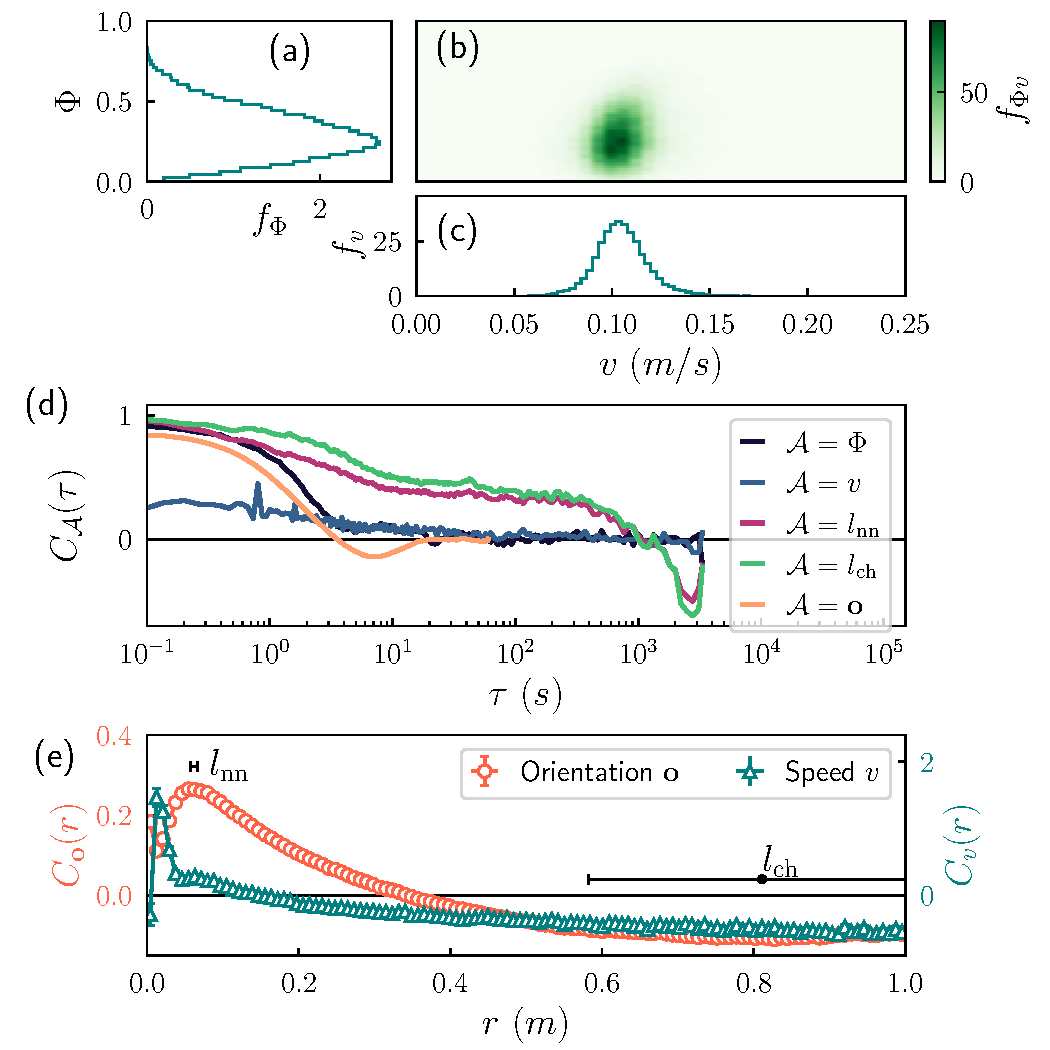
\includegraphics[width=\linewidth]{dynamics-2d-50}
  \caption[The dynamics of 50 fish in 2D]{
  	The dynamics of 50 adult zebrafish in 2D.
  	(a) The probability density function ($f_\Phi$) of the polarisation ($\Phi$, Eq.~\ref{eq:polarisation}).
  	(b) The joint probability density function ($f_{\Phi v}$) for the polarisation ($\Phi$) and the speed ($v$).
  	(c) The probability density function ($f_v$) of the average speed (Eq.~\ref{eq:speed}).
  	(d) The auto-correlation function, $C_\mathcal{A}(\tau)$, of the the polarisation ($\Phi$), the average speed ($v$), the nearest neighbour distance ($l_\mathrm{nn}$), the effective convex hull diameter ($l_\mathrm{ch}$), and the orientation of each fish ($\mathbf{o}$).
  	(e) The connected correlation function of the orientation ($\mathbf{o}$) and speed ($v$), as a function of pairwise distances.
  }
  \label{fig:dynamics-2d}
\end{SCfigure}


On the other hand, the relaxation of the local density, as probed by the ACFs of $l_\mathrm{nn}$ and $l_\mathrm{ch}$, is a much slower process. The two ACFs have two similar relaxation timescales of 900s (15 minutes). This process might corresponds to the fragmentation of the group. As a result, we use this largest timescale ($\tau_\rho \sim$ 900s) to characterise the time it took for 50 zebrafish to forget their state, in a quasi-2D experiment.

The connected correlation function of the fish, for their speed as well as their orientation was plotted in Fig.~\ref{fig:dynamics-2d}(e). Surprisingly, the correlation function of the orientation, $C_\mathbf{o}(r)$, exhibits a much longer correlation length ($\xi_\mathbf{o} \sim 0.38m$), compared to the correlation of the speed ($\xi_v \sim 0.15m$). This picture is very different from European starlings, whose correlations lengths for both orientation and speed were similar \cite{cavagna2010}. Our result suggests the lack of speed synchronisation for the zebrafish, which could be the reason that the fish were always in a randomised state with a low $\Phi$ value.




\subsection{The Changing States}
\label{section:change-states-2d}

Since the fish change their (macroscopic) states in a timescale of 15 minutes, we segment the trajectory into different sections with the duration of 15 minutes. By doing so, we could study the structure and dynamics of the fish as a function of time, since the fish could change their states continuously, rather than being in a steady state.

The changing states of the fish as a function of observation time as plotted in Fig.~\ref{fig:change-states-2d}. The $g(r)$ of the fish were shown in Fig.~\ref{fig:change-states-2d}(a), were the peak of the $g(r)$ gradually decreases with the evolution of time. This suggests a decrease of cohesiveness for the fish group. The ACF of the orientation of the fish, $C_\mathbf{o}(t)$, at different time were plotted in Fig.~\ref{fig:change-states-2d}(b), which exhibit less variation comparing with the $g(r)$ functions.

 \begin{SCfigure}
  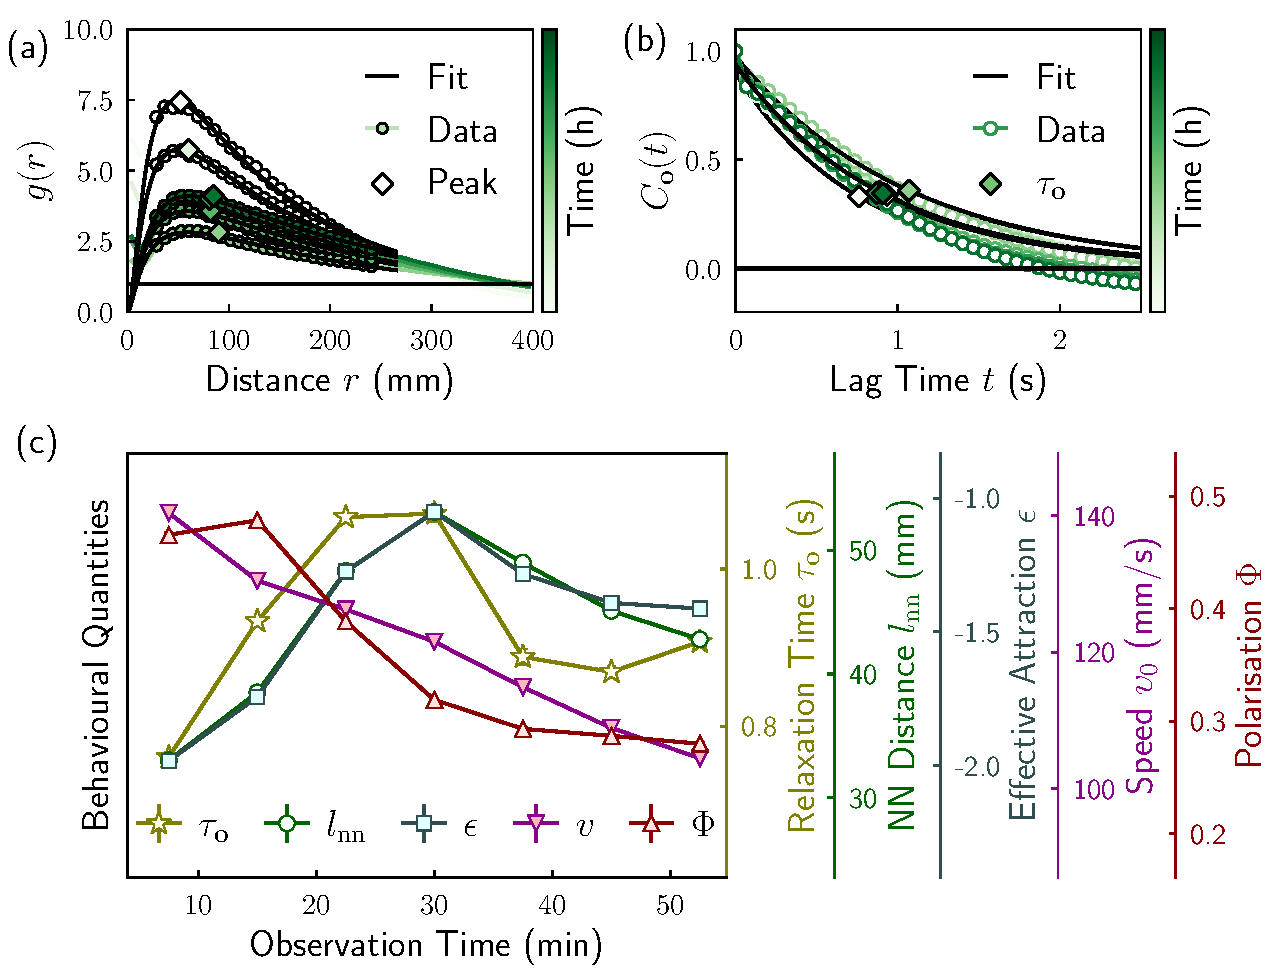
\includegraphics[width=\linewidth,outer]{change-states-2d-50}
  \caption[The behavioural descriptors of 50 zebrafish]{
  	(a): The auto--correlation function of the polarisation and average speed of the fish group.
	(b): The auto--correlation function of the orientations of fish.
	(c): Sequence of radial distribution functions with increasing time: at early times (top curves) the fish are clustered together so that the peak is large; at later times (bottom curves) the local density decreases and so does the peak height.
	(d): The time evolution of the averaged {\descriptors} for 50 {\smallfish} fish. Each point corresponds to the average value in 15 minutes.
	The error bars illustrate the standard error values.
  }
  \label{fig:change-states-2d}
\end{SCfigure}


The time evolution of 5 selected behavioural quantities, the orientational relaxation time ($\tau_\mathbf{o}$, Eq.~\ref{eq:tau}), the nearest neighbour distance ($l_\mathrm{nn}$, Eq.~\ref{eq:nnd}), the effective attraction ($\epsilon$, Eq.~\ref{eq:effective-attraction}), the average speed ($v$, Eq.~\ref{eq:speed}), and the polarisation ($\Phi$, Eq.~\ref{eq:polarisation}), was plotted in Fig.~\ref{fig:change-states-2d}(c). Each point in Fig.~\ref{fig:change-states-2d}(c) corresponds to the time average over 15 minutes. It is clear that the structural quantities ($\epsilon$ and $l_\mathrm{nn}$) were correlated while the dynamical quantities ($v$ and $\Phi$) were correlated.

Surprisingly, the orientational relaxation time seems to correlate with the structural quantities, and the fish exhibit slower orientation relaxation when they were in a less cohesive state. One possible explanation is that the orientation of the fish will be interrupted by a close neighbour, as a consequence of the avoidance for collision. These extra interruptions, on top of the intrinsic orientational diffusion of the fish, make the fish change their orientations faster in a dense group. This picture is also consistence with the observation that the polarisation of the fish increase as the nearest neighbour distances of the fish increase \cite{miller2012}.


\section{The Behaviour of 50 Zebrafish in 3D}

Following the same data processing procedure and analysis, we also studied the behaviour of 50 zebrafish in a 3D observation. In contrast to the 2D experiments where the fish were confined in a shallow water environment, now the fish can explore a 3D space enclosed by the water-air interface and a bowl-shaped tank.

\subsection{The Structure}
\label{section:analysis-structure-3d}


The spatial distribution of 50 zebrafish was shown in Fig.~\ref{fig:structure-3d} (a), where the joint distribution of the $x$ and $z$ coordinate clearly shows the depth preference of the fish, as discussed in section~\ref{section:fish_many_3d}. With the ideal gas sampled according to the distribution of the fish, we calculated the PDF of the pairwise distances, $f_d(r)$, of the fish and the ideal gas. The result is shown in Fig~\ref{fig:structure-3d}(b). It is clear that the fish are more cohesive, as the mode of $f_d^\mathrm{fish}(r)$ locates at a smaller distance value.

The ratio of two PDFs gives the $g(r)$ (Eq.~\ref{eq:gr}), presented in Fig.~\ref{fig:structure-3d}(c). Like the 2D results (Fig.~\ref{fig:structure-2d}), the $g(r)$ exhibits a typical disordered, fluid-like shape, featuring a single peat at $\sim l_\mathrm{nn}$ with a monotonic decay. The height of the peak reaches the value of 5, being larger than the peak height ($\sim 2.2$, Fig.~\ref{fig:structure-2d}(c)) in the 2D experiment. This difference indicates that the 50 fish were swimming in a more cohesive way in the 3D experiment, comparing with the 2D experiment.


Importantly, the correlation length of the density ($\xi_\rho$, Eq.~\ref{eq:length-density}) is close to the effective convex hull diameter ($l_\mathrm{ch}$, Eq.~\ref{eq:convex-hull-diameter}), as shown in Fig.~\ref{fig:structure-3d}. This suggests the fish remained a compact, and cohesive group in the 3D experiment. A snapshot of such a cohesive group was plotted as circular markers in Fig.~\ref{fig:structure-3d} (a).

Since the fish always form a compact cluster, a cohesive clique, when they were swimming in the 3D observation tank, there is no void in the length scale of the convex hull of the group. Comparing with the size of the explorable environment, the $l_\mathrm{ch}$ is mush smaller, and the void corresponds to the space where the fish aggregation could explore collectively.

The cohesive nature of the fish in the 3D experiment is also supported by the distribution of the $l_\mathrm{ch}$ shown in Fig.~\ref{fig:structure-3d}, which is much narrower than that from the 2D experiments. Interestingly, the distribution of $l_\mathrm{nn}$ for the fish swimming in both 3D and 2D environments were close. Numerically, the averaged $l_\mathrm{nn}$ value for the 3D experiments were slightly smaller than the value from 2D experiments (Table~\ref{table:behaviour}).


\begin{SCfigure}
  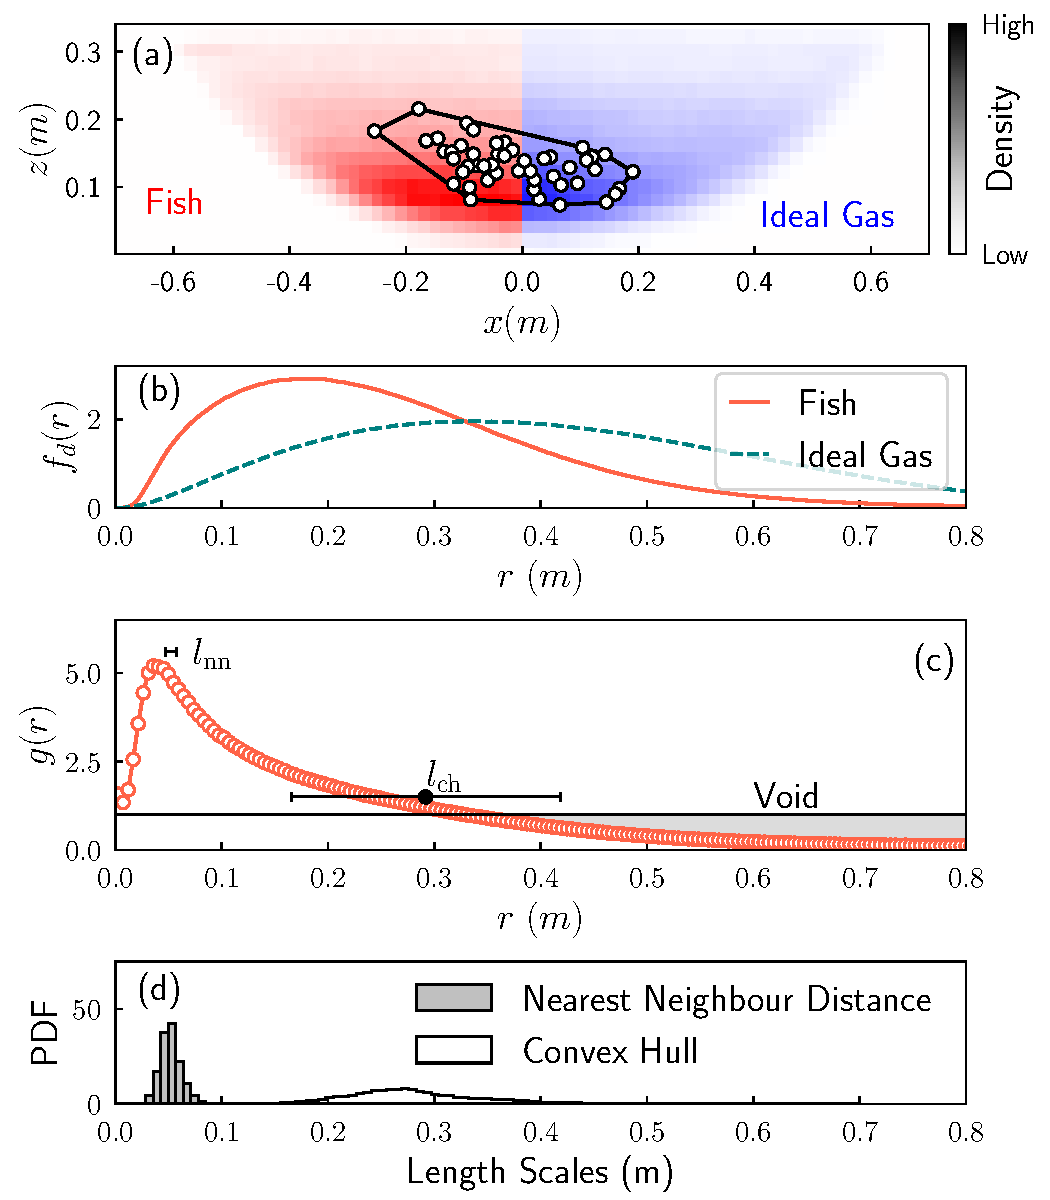
\includegraphics[width=\linewidth]{structure-3d-50}
  \caption[The structure of 50 fish in 3D]{
  	The structure of 50 adult zebrafish in 3D.
  	(a) The joint distribution of the $x$ and $z$ coordinates of the fish and the ideal gas particles. The distribution of the ideal gas is biased to be identical to the fish. The location of 50 fish at one time point is plotted as circles. The boundary convex hull of these 50 scatters is plotted as solid lines.
  	(b) The probability density function of the pairwise distributions for the fish and the ideal gas particles.
  	(c) The radial distribution function, $g(r)$ (Eq.~\ref{eq:gr}) of the fish. It is defined as the ratio between the two PDFs in (b). Two important length scales, the nearest neighbour distance and the size of the convex hull were captured by the $g(r)$. The long distance region where $g(r) < 1$ corresponds to the void in the tank, where the group were able to explore.
  	(d) The distribution of the nearest neighbour distance and the effective diameter of the convex hull, of the fish.
  }
  \label{fig:structure-3d}
\end{SCfigure}

\subsection{The Dynamics}


The dynamics of the 50 zebrafish in a 3D observation experiment is shown in Fig.~\ref{fig:dynamics-3d}. Figure~\ref{fig:dynamics-3d} (a)-(c) shows the distribution of the speed ($v$) and the polarisation ($\Phi$), as well as the joint distribution of the two. Interestingly, the speed exhibits a bimodal distribution (Fig.~\ref{fig:dynamics-3d}), indicating the fish were changing between a slow state to a fast state during the observation. The joint PDF of $v$ and $\Phi$ exhibits a positive correlation, as shown in Fig.~\ref{fig:dynamics-3d}(b).


The ACF of different structural quantities and dynamical quantities for 50 fish were plotted in Fig.~\ref{fig:dynamics-3d}(d). Like the 2D results, these ACFs exhibit two decays, featuring the relaxation of the orientation ($\tau_\mathbf{o} \sim 1s$) and the local density ($\tau_\rho \sim 120s$). The latter timescale is used to separate the observation into separate segments, to study the time evolution of the fish states in section~\ref{section:change-states-3d}.


\begin{SCfigure}
  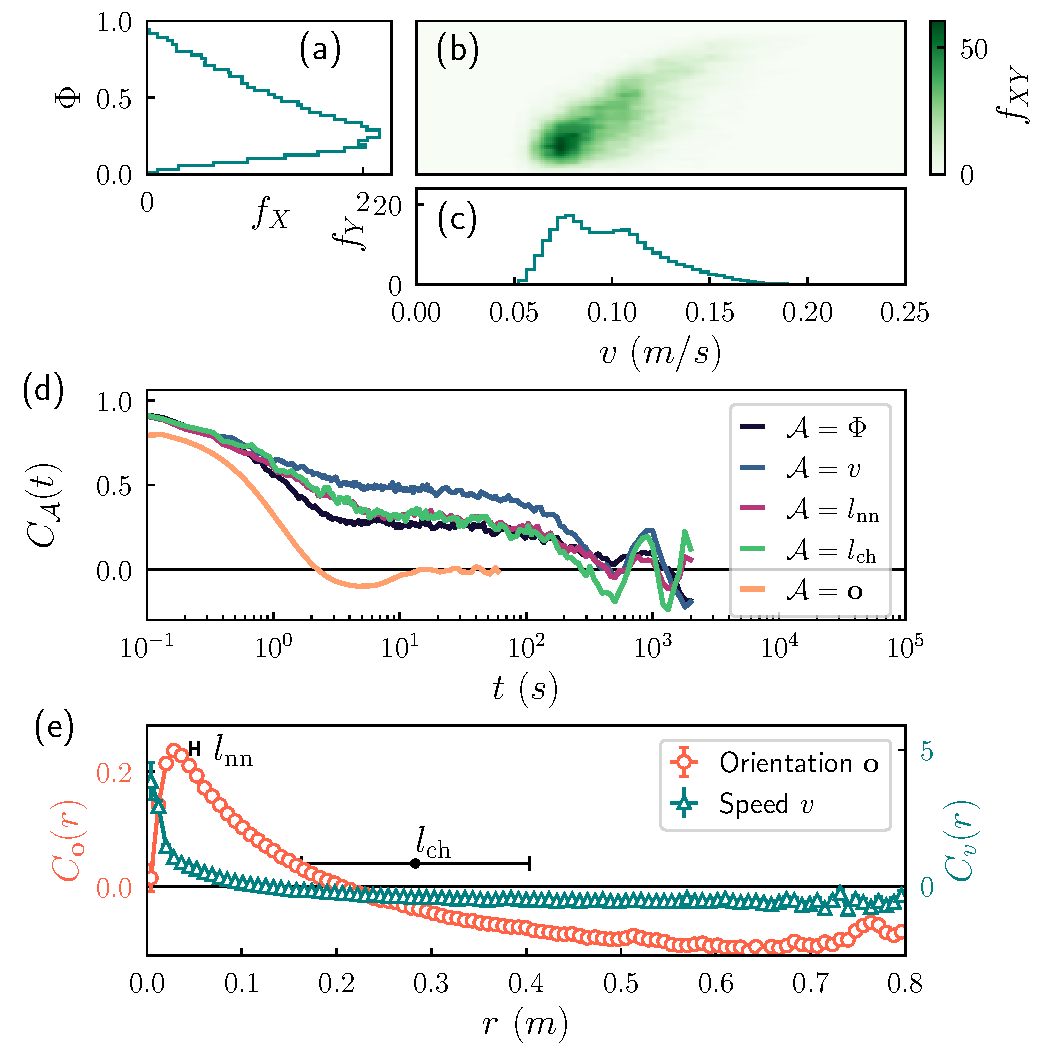
\includegraphics[width=\linewidth]{dynamics-3d-50}
  \caption[The dynamics of 50 fish in 3D]{
  	The dynamics of 50 adult zebrafish in 3D.
  	(a) The probability density function ($f_\Phi$) of the polarisation ($\Phi$, Eq.~\ref{eq:polarisation}).
  	(b) The joint probability density function ($f_{\Phi v}$) for the polarisation ($\Phi$) and the speed ($v$).
  	(c) The probability density function ($f_v$) of the average speed (Eq.~\ref{eq:speed}).
  	(d) The auto-correlation function, $C_\mathcal{A}(\tau)$, of the the polarisation ($\Phi$), the average speed ($v$), the nearest neighbour distance ($l_\mathrm{nn}$), the effective convex hull diameter ($l_\mathrm{ch}$), and the orientation of each fish ($\mathbf{o}$).
  	(e) The connected correlation function of the orientation ($\mathbf{o}$) and speed ($v$), as a function of pairwise distances.
  }
  \label{fig:dynamics-3d}
\end{SCfigure}


The connected correlation function of the speed and orientation of the fish, $C_v(r)$ and $C_\mathbf{o}(r)$, was presented in Fig.~\ref{fig:dynamics-3d}(e). Being very similar to the 2D results, the orientation of the fish exhibits a longer correlation length compared with the speed. The two correlation length values, $\xi_\mathbf{o}$ and $\xi_v$, are listed in Table~\ref{table:behaviour}.

Comparing with the 2D results in Fig.~\ref{fig:dynamics-2d}, the fish were swimming at a similar speed in a 3D environment, with $v_\mathrm{2D} = 0.11m/s$ and $v_\mathrm{3D} = 0.098m/s$. However, the fish were swimming in a more ordered way in a 3D observation, indicated by the high $\Phi$ values at the tail of the distribution $f_\Phi$. 
It is notable that the ACFs of the structural quantities ($l_\mathrm{nn}$ and $l_\mathrm{ch}$) and dynamical quantities ($\Phi$ and $v$) sharing the same shape for the fish in the 3D observation. This similarity of the ACFs was not observed in the 2D experiments.

%The fact that the fish presents different behaviour with varying degrees of order was also observed by \citeauthor{miller2012}, where the movement of zebrafish changed from ordered to disordered over time \cite{miller2012}.


\subsection{The Changing States}
\label{section:change-states-3d}

\begin{SCfigure}
  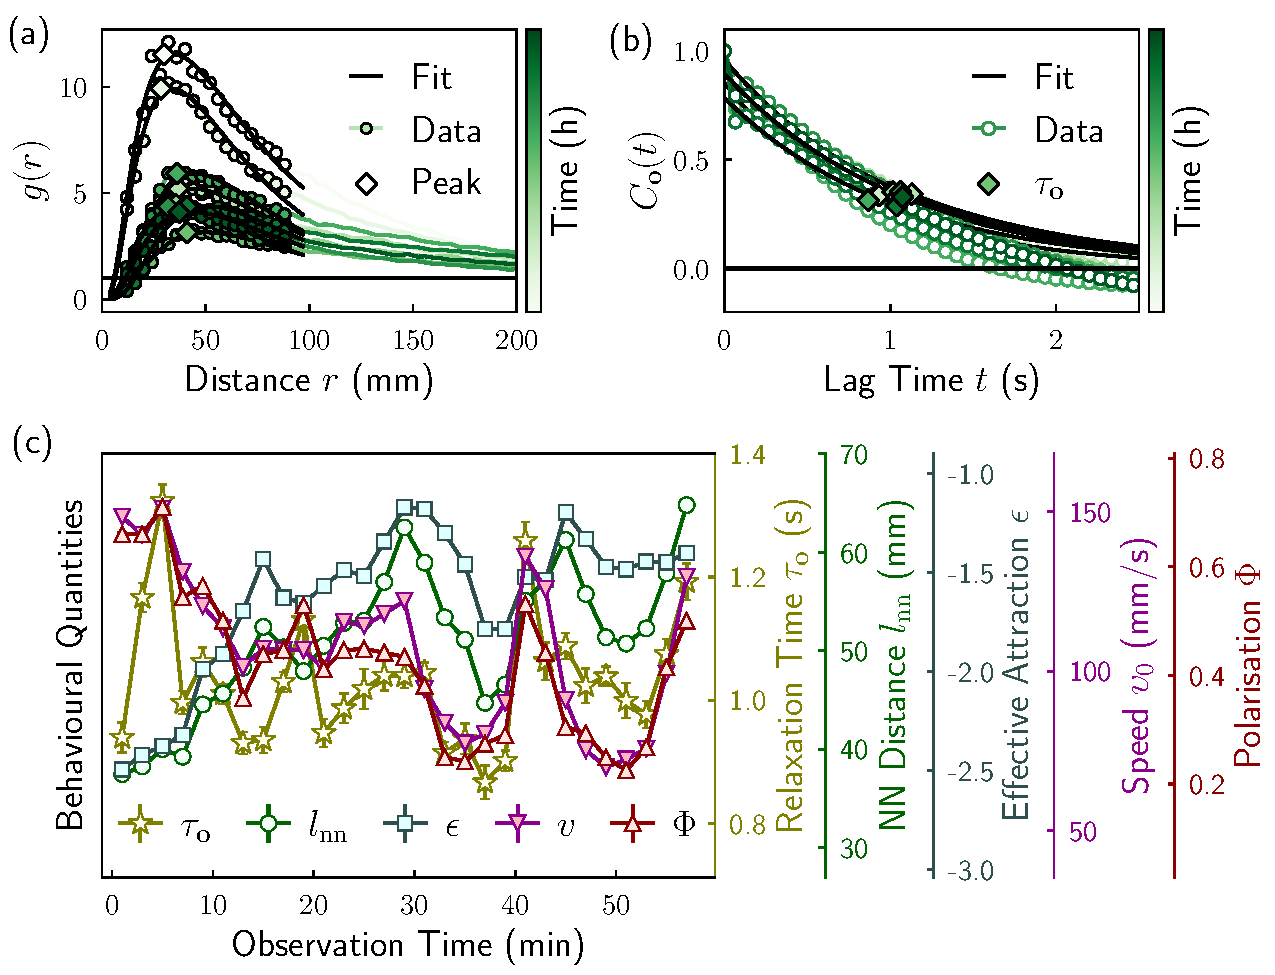
\includegraphics[width=\linewidth,outer]{change-states-3d-50}
  \caption[The behavioural descriptors of 50 zebrafish]{
  	(a): The auto--correlation function of the polarisation and average speed of the fish group.
	(b): The auto--correlation function of the orientations of fish.
	(c): Sequence of radial distribution functions with increasing time: at early times (top curves) the fish are clustered together so that the peak is large; at later times (bottom curves) the local density decreases and so does the peak height.
	(d): The time evolution of the averaged {\descriptors} for 50 {\smallfish} fish. Each point corresponds to the average value in 2 minutes.
	The error bars illustrate the standard error values.
  }
  \label{fig:change-states-3d}
\end{SCfigure}

To study the changing states of the fish group, we separated the observation into short segments of 120s, and analyse the behaviour of the fish in these short periods separately. The results are shown in Fig.~\ref{fig:change-states-3d}. 
For each segment, we calculated the ACF of the orientation, as shown in Fig.~\ref{fig:change-states-3d} (b), as well as the $g(r)$, as plotted in Fig.~\ref{fig:change-states-3d}(c). From these two correlation functions, we extracted the changing $\tau_\mathbf{o}$ and the changing effective attraction ($\epsilon$) values. Like the behaviour of fish during our 2D observation, the cohesion among the fish gradually decreases, indicated by the decreasing height of the peak in the $g(r)$. However, no systematic change of the $C_\mathbf{o}(t)$ were observed.

The time evolution of different structural and dynamical quantities were plotted in Fig.~\ref{fig:change-states-3d}(d). All these quantities change with time, indicating the fish were constantly changing their states.
The speed is correlated with the polarisation, and the nearest neighbour distance is correlated with the effective attraction.


These correlations were also observed from our 2D experiments in Fig.~\ref{fig:change-states-2d}. The non-linear nature of the time-evolution of fish states revealed the complexity of the behaviour of the fish, and more controlled experiments is necessary to differentiate the possible origins, that are responsible for the changing states of the fish. For instance, a sudden noise in the environment might trigger the jump in speed in Fig.~\ref{fig:change-states-3d}. But such change, termed as the spontaneous startle cascades in \cite{rosenthal2015}, might also emerge naturally without any triggering factor.





\section{The Universal Behaviour of Zebrafish}
\label{section:universal}


The complicated changing states of the fish shown in Figs.~\ref{fig:change-states-2d} and \ref{fig:change-states-3d}, can be captured by one number, regardless of the dimension of the swimming environment. This number is termed as the \emph{reduced persistence length} (\gls{kappa}), whose definition is,

\begin{equation}
	\kappa 
	= \frac{v \tau_\mathrm{o}}{l_\mathrm{nn}}
	= \frac{l_p}{l_\mathrm{nn}}	.
\label{eq:kappa}
\end{equation}

\noindent The value of $\kappa$ correlates robustly with the value of polarisation $\Phi$, as shown in Fig.~\ref{fig:states-1d}.
This correlation is remarkable because it describes all the experimental observations on different adult zebrafish groups, with different ages.
%This robust correlation is the most important result in this thesis.
A very simple argument for the correlation is that each fish could share its current moving direction with the group, in the lengthscale of $l_p$. Such information could be transmitted to more members in a cohesive group, with smaller $l_\mathrm{nn}$ value. When more members were exchanging their information about the moving direction, the entire group is more likely to form a consensus, and exhibit ordered movement with a high $\Phi$ value.

This explanation is helpful because it relates the property of the individual fish (the persistence length, and the local density) to the macroscopic behaviour (the polarisation).
Such connection is vital to understand the behaviour of mutant zebrafish, which had significantly larger $l_p$ values comparing with the wildtype zebrafish. The relevant results will be presented in chapter~\ref{chapter:fish_mutation}.
In addition, it is easy to compare the observed experimental result in Fig.~\ref{fig:states-1d} with the computer simulations of agent-based models, since both $\kappa$ and $\Phi$ are dimensionless numbers. Such comparison will be discussed in chapter~\ref{chapter:fish_model}.


 \begin{SCfigure}
  \includegraphics[width=\linewidth,outer]{states-1d}
  \caption[The behaviour of 50 zebrafish described by reduced persistence length]{
  	The relationship between the polarisation, the order of the movement, and the reduced persistence length of the fish. For the 3D observation, multiple repeated measurement with different fish groups at different dates were collected (Y1-Y4: different young fish groups; O1-O4: different old fish groups).
  	All of the observed fish behaviour results were collapsed onto a master curve. The result of one 2D observation was also included, as open circles. The 2D results does not collapse onto the same master curve from the 3D data, because of the difference in the dimensions.
  }
  \label{fig:states-1d}
\end{SCfigure}

\vfill
\pagebreak

\begin{adjustwidth}{-5cm}{0cm}
\begin{tcolorbox}[
fonttitle=\sffamily\Large,
right=0.05\linewidth,
title=Summary of Chapter~5
]
\begin{itemize}
	\item We discussed the methods to analyse the experimental coordinates of the zebrafish, in order to study their collective behaviour. There are four steps.
	\begin{description}
		\item[1. Refining Coordinates] \hfill \\
		Some coordinates are very close to each other, which are physically impossible. These overlapping particles can be removed with an optimisation algorithm.
		\item[2. Linking Coordinates into Trajectories] \hfill \\
		The refined coordinates can be linked into trajectories, and the short trajectories can be extended using methods in section~\ref{section:link}.
		\item[3. Analysing the Structure of the Fish Group] \hfill \\
		We use the nearest neighbour distance ($l_\mathrm{nn}$), the size of the convex hull ($l_\mathrm{ch}$), and the radial distribution function $g(r)$ to characterise the structure of the fish group.
		\item[4. Analysing the Dynamics of the Fish Group] \hfill \\
		We use the average speed ($v$), the polarisation ($\Phi$), the relaxation time scales ($\tau$) to characterise the dynamics of the fish group.
		In addition, we use the correlation functions of the orientation and the speed, $C_\mathbf{o}(r)$ and $C_v(r)$, to measure the dynamical lengthscales.
		\end{description}
	\item We get the following results from the 2D movement of 50 zebrafish.
	\begin{itemize}
		\item The fish groups segmented into sub-clusters.
		\item The fish groups were in the disorder phase, with low polarisation values.
		\item The collective motion of the fish groups exhibited a short time scale related to the reorientation of the fish individual (1 s), and a large time scale related to the relaxation of the local density (15 minutes).
		\item The correlation length of orientation is longer than the correlation length of the speed.
		\item The macroscopic state of the fish group changes over time, indicated by the changing quantities in Fig.~\ref{fig:change-states-2d}.
	\end{itemize}
	\item  We get the following results from the 3D movement of 50 zebrafish.
	\begin{itemize}
		\item The fish group remained a cohesive cluster without fragmentation.
		\item The fish group switched between the ordered phase and the disorder phase, with varying polarisation values.
		\item The collective motion of the fish group exhibit a short time scale related to the reorientation of the fish individual (1 s), and a large time scale related to the relaxation of the local density (2 minutes).
		\item The correlation length of orientation is larger than the correlation length of the speed.
		\item The macroscopic state of the fish group changes over time, indicated by the changing quantities in Fig.~\ref{fig:change-states-3d}.
	\end{itemize}
	\item The change of the macroscopic states of the zebrafish groups is not totally random. The ratio between the persistence length and the nearest neighbour distance, for both 2D and 3D data, presents a robust correlation with the polarisation.
\end{itemize}
\end{tcolorbox}
\end{adjustwidth}


\end{document}

\documentclass[11pt,twoside]{report}
\usepackage{preamble}
\graphicspath{{../img/ch6/}}
\setcounter{chapter}{5}

\begin{document}

\chapter{Modelling Zebrafish}
\label{chapter:fish_model}


\epigraph{人相忘乎道术}{庄子}


\section{Introduction}

In this chapter we will study the behaviour of the zebrafish with the help of computer simulation. The goal of the simulation is to reproduce the experimental results from chapter~\ref{chapter:fish_2d} to chapter~\ref{chapter:fish_analysis}.
We will use the Monte-Carlo simulation to study a system in equilibrium, in order to reproduce the spatial distribution of the fish under the influence of the boundary, the gravity, as well as the pairwise interaction.
In addition, we will use a dynamical simulation to study an agent-based\marginfootnote{
The dynamical simulation is similar to the Brownian dynamics simulation for the liquid, where all the particles were updated according the force exerted on them. It's different from the Monte-Carlo simulation where the particles are moved randomly.
The moving individuals in the model can take different names, like the ``particles'', ``animals'', and ``agents''. The term ``agents'' will be used in this chapter for consistency.
} active matter model, in order to recreate the dynamical feature of the fish group in the experiments.
%The purpose of these simulations is to understand and explain the observed zebrafish behaviour, so that we could get more insights into its nature. 
%In particular we focus on the distribution of the density, as well as the order of the dynamics.

The density distribution of the fish was strongly affected by the presence of the boundary, as the fish were physically constrained in the tank.
For the 3D experiment, the distribution of the fish was also affected by an ``effective gravity'', as well as the holes drilled on the tank. These environmental factors can be treated as external fields affecting the fish. In addition to these external factors, the fish-fish interaction will also change their distribution.
With the Monte-Carlo (\gls{MC}) simulation techniques, we can study these effects individually. By doing so, we implicitly tested the idea of mapping active matter system to an equilibrium counterpart, where the non-equilibrium feature of the system, the activity, was summarised by an effective temperature\marginfootnote{
This ``effective equilibrium'' picture is supported by the exponential decay of the excess distribution function shown in section~\ref{section:fish_1_3d}, as the decay suggests the Boltzmann-like distribution commonly seen in equilibrated systems.
} \cite{palacci2010, klongvessa2019}.

For a group of fish, the order of their dynamics, captured by the polarisation value (Eq.~\ref{eq:polarisation}), correlates robustly with a non-dimensional value \gls{kappa}, the ratio between the persistence length (\gls{lp}) and the nearest neighbour distance (\gls{lnn}).
Such a correlation suggests the local density and the persistence motion of the fish dominated the polarisation of the system.
Since the persistence motion is a proxy to the \emph{activity} of the fish, the entire group of 50 zebrafish is behaving like an alignment dominated active matter system (section~\ref{section:active-phase}).
To confirm the similarity of a group of zebrafish, and a model active matter system, we will use the dynamical simulation method to simulate the famous active matter model, the Vicsek model.
To get a good fit between the model and the experiments, we will have to modify the Vicsek mode and consider the orientational inertia of the fish.
The fitting of the model and the experimental result suggests the existence of the effective alignment interaction among the fish. And the changing states of the fish could be understood as a change of the noise level for the model.


\section{Simulation Methods}


\subsection{General Idea}

If we think of fish as a collection of agents following pre-defined movement rules, we could reproduce the movement of the fish with the computer simulation. Formally, we call a collection of agents a \emph{system}. And the system can change its (microscopic) states over time.
By observing the system for a long time, we could obtain the trajectory of the system, and then calculate the quantities that we are interested in (see chapter~\ref{chapter:fish_analysis} for examples). Such process is summarised in the following algorithm (Algorithm~\ref{alg:simulation}).
During the simulation, the system change its states under some constraints. For example, the constraints could be a controlled noise level (\gls{beta}), a constant number density (\gls{rho}), and a fixed total number (\gls{N}) of agents.


\begin{algorithm}
	\KwData{Constraints $\{ \beta, \rho, N, \dots \}$}
	\KwResult{Trajectory}
	System $\gets$ initial microscopic state with $\{ \beta, \rho, N, \dots \}$\;
	\Repeat{System is stable, and forgets the initial microscopic state}{
		change the microscopic state of the system with $\{ \beta, \rho, N, \dots \}$
	}
	Trajectory $\gets \emptyset$\;
	\Repeat{
		The statistics are good enough
	} {
		change the microscopic state of the system with $\{ \beta, \rho, N, \dots \}$\;
		Put current state in Trajectory\;
	}
\caption{The Simulation Procedure}
\label{alg:simulation}
\end{algorithm}

\subsection{Monte-Carlo Simulation}

There are multiple ways to change the state of the system in algorithm~\ref{alg:simulation}. In a seemly arbitrary fashion, we could change the state of the system randomly, and reject some states that is unlikely to happen. This method is termed ``Monte-Carlo'' (MC) simulation, and the acceptance ratio were often determined by the Metropolis algorithm. Typically, the acceptance ratio from state $\zeta$ to $\nu$, \gls{acc}, is written as

\[
	A(\zeta \rightarrow \nu) = \left\{
		\begin{array}{ll}
			\exp\left(-\beta(E_\nu - E_\zeta)\right)
			& \mbox{if $E_\nu - E_\zeta > 0$}\\
			1 & \mbox{otherwise.}
		\end{array}
	\right.
\]

\noindent And the values of $E_\nu$ and $E_\zeta$ represent the energy values of state $\nu$ and $\zeta$, respectively. The value $\beta$ is the inverse temperature. The smaller $\beta$ value is, the higher the temperature, and the larger randomness the system exhibits.

With MC simulation, it is easy to constrain the agents in the fish tank, by setting $E = \infty$ once an agent is outside the tank.\marginfootnote{
Operationally, we reject the states if any agent is outside the fish tank.
} In addition, the effect of external fields, like gravity, can be added easily to the simulation. However, due to the lack of ``true'' dynamics in the MC simulation, we will not have access to the velocities of the system. Hence, this simulation method is only used to model the spatial distribution of the zebrafish.


\subsection{Dynamical Simulation}


Another way to change the state of the system is to integrate the \emph{equation of motion} of all the agents. For animals, the equations to be integrated represent the behavioural rules of the agents.
Being different from the conventional molecular dynamics simulation or mesoscale simulations \cite{allen2017}, the simulation of animal behaviour often incorporates more eccentric rules, such as a fixed vision zone\cite{couzin2002, yigit2020}, and an attraction to the group centre \cite{reynolds1987}. Generally, the updating rules for the agents could be described by the following equation,

\begin{equation*}
\begin{split}
	\mathbf{v}_{i}^{t+1}
	&= \mathcal{B} [\mathbf{v}_{i}^t] \\
	\mathbf{x}_i^{t+1}
	&= \mathbf{x}_i^{t} + \mathbf{v}_i^{t+1},
\end{split}
\end{equation*}

\noindent where the operator $\mathcal{B}$ encodes all the behavioural rules of the animals. By changing the coordinates and velocities of all the agents simultaneously, we change the state of the system (Algorithm~\ref{alg:simulation}).


\section{The Distribution of the Density}
\label{section:simulate-density}

In this section we will model the spatial distribution of the fish in the 3D experiment. The simulation will illuminate the effects of the environmental factors, such as the fish tank and the gravity. By comparing with the experimental density distribution, we can get phenomenological parameters such as the effective temperature, to describe the behaviour of the fish.



\subsection{The Effect of the Tank}
\label{section:sim-mc-tank}

The 3D geometry of the tank confining the zebrafish was determined in section \ref{section:system_3d}, and the shape of the tank can be expressed as,

\begin{equation*}
	z = c r^2,	
\end{equation*}


\noindent where $c=0.74 m^{-1}$ when both $r$ and $z$ were expressed in the unit of meters. The volume (\gls{vol}) of the tank can be calculated as

\begin{equation*}
	V = \int_{0}^{h}{\pi \frac{z}{c}} dz
	  = \frac{\pi h^2}{2 c},	
\end{equation*}


\noindent where $h$ is the height of the tank, the vertical distance between the water surface and the base of the tank. The joint probability density function (PDF) of random points, being uniformly distributed inside the tank, is written as,

\begin{equation*}
	f(x, y, z) = V^{-1} = \frac{2c}{\pi h^2}.		
\end{equation*}

\noindent The joint PDF of the uniform distribution can be expressed in the spherical coordinates as,

\begin{equation}
	f(\theta, r, z) = \frac{2c}{\pi h^2} r,
\label{eq:density-pdf-tank}
\end{equation}

\noindent where $\theta$ is the azimuthal angle, $r = \sqrt{x^2 + y^2}$ is the radius in $XY$ plane.  From the expressions above, we can calculate the marginal distribution of $r$ and $z$ coordinates:

\begin{equation}
\begin{split}
	f_R(r) &= \int_0^{2\pi}{d \theta} \int_{cr^2}^{h}{dz} \; f(\theta, r, z)
		= \frac{4c}{h} r - \frac{4 c^2}{h^2} r^3, \\[2em]
	f_Z(z) &= \int_0^{2\pi}{d \theta} \int_0^{\sqrt{z/c}}{dr} \; f(\theta, r, z) 
	= \frac{2}{h^2} z.
\end{split}
\label{eq:dist-tank}
\end{equation}

\noindent The analytical result (Eq.~\ref{eq:dist-tank}) is checked against the numerical sampling of random points inside the tank, as shown in Fig.~\ref{fig:dist-tank}. These PDFs can be used as comparison for the distribution of real fish data, as presented in section~\ref{section:observe-3d-result}. The experimental distribution of the fish is very different from the ideal gas distribution.

\begin{SCfigure}
  \includegraphics[width=\linewidth]{density-tank}
  \caption[The 3D geometry of the experimental fish tank]{
  The marginal probability density distribution of points sampled uniformly inside the experimental fish tank.
  Left: the distribution the planar radius $r$.
  Right: the distribution of the $z$ component of the points.
  }
  \label{fig:dist-tank}
\end{SCfigure}


\subsection{The Effect of the ``Gravity''}
\label{section:sim-mc-gravity}

From the results presented in section~\ref{section:observe-3d-result}, it is evident that the zebrafish will be affected by an ``effective gravity'', because of their depth preference behaviour.
This effective gravity is similar to 
As a first attempt, we could calculate the density distribution of ideal gas particles in equilibrium, with an Boltzmann weight $\exp(-\beta z)$ to capture the effect of the gravity.
The \emph{partition function} (\gls{Z}) of the system is written as,

\begin{equation*}
	Z = \int_0^h \pi \frac{z}{c} \exp(-\beta z) dz
      = \frac{\pi (1 - \exp(-\beta h) (1 + \beta h))}{c \beta^2}.
\end{equation*}

\noindent With the partition function, we could then calculate the joint probability density function of the ideal gas, in the spherical coordinate system (similar to Eq.~\ref{eq:density-pdf-tank}).

\begin{equation}
	f(\theta, r, z)
	= \frac{r \exp(-\beta z)}{Z}
	= \frac{c \exp(-\beta z) r \beta^2}
	{\pi(1 - \exp(-\beta h)(1 + \beta h))}
\label{eq:density-pdf-gravity}
\end{equation}

\noindent where $\beta = 1 / (k_B T)$ is the inverse temperature. For a physical systems in equilibrium, the vale of \gls{beta} relates to the real temperature measured by a thermometer. However, the value of $\beta$ for the fish only controls the level of randomness of the system, without a concrete physical meaning. From the function $f(\theta, r, z)$, we can calculate the distribution functions $f_R(r)$ and $f_Z(z)$:

\begin{equation}
\begin{split}
	f_R(r) &= \int_0^{2\pi}{d \theta} \int_{cr^2}^{h}{dz} \; f(\theta, r, z)
		= \frac{
			2 c \left(
					\exp \left( \beta (h - c r^2) \right) - 1
				\right) r \beta
		}{
			\exp(\beta h) - \beta h - 1
		}, \\[2em]
	f_Z(z) &= \int_0^{2\pi}{d \theta} \int_0^{\sqrt{z/c}}{dr} \; f(\theta, r, z) 
	= \frac{\exp(-z \beta) z \beta^2}{
		1 - \exp(-\beta h) (1 + \beta h)
	}.
\end{split}
\label{eq:dist-gravity}
\end{equation}

\noindent The results from Eq.~\ref{eq:dist-gravity} were checked against the Monte-Carlo simulation results, as shown in Fig.~\ref{fig:dist-gravity}. With the increase of $\beta$, hence the decrease of temperature, the agents were pushed towards smaller $z$ values and $r$ values. By ``fitting'' the experimental results with the analytical results from Eq.~\ref{eq:dist-gravity}, and setting $\beta$ as a free parameter, we could obtain the effective temperature for the fish.
%A systematic study of the change of the effective temperature could give us a more systematic understanding of the depth preference of the zebrafish. For instance, the fitting parameter $\beta$ could be interpreted as the ``fear'' perceived by the fish.

\begin{SCfigure}
  \includegraphics[width=\linewidth]{density-gravity}
  \caption[The distribution of ideal gas in the tank subjected to gravity]{The marginal probability density distribution of ideal gas particles sampled uniformly inside the experimental fish tank, where the particles were subjected to the gravity field. Left: the distribution the $z$ component. Right: the distribution of the $r = \sqrt{x^2 + y^2}$. The scatters were result of Monte-Carlo simulations, and the solid lines were from Eq.~\ref{eq:dist-gravity}.}
  \label{fig:dist-gravity}
\end{SCfigure}


\subsection{The Effect of the Holes}
\label{section:sim-mc-holes}

In our 3D fish observation experiments, the holes on the tank disrupted the density distribution of the fish. This disruption makes the result in Eq.~\ref{eq:dist-gravity} very different from the distribution of the fish, as shown in section~\ref{section:holes}. To mimic such effect, we could model holes as an extra field, with the following form,

\begin{equation}
	H(r, z) = q
		\sum_i{\frac{
		\left[
			(r - r_i)^2 + (z - c r_i^2)^2
		\right]^{-2}
		}{r_i}},
\label{eq:energy-holes}
\end{equation}

\noindent where $r_i$ represents the location of the holes on the tank. Specifically, there are three sets of holes (Fig.~\ref{fig:density-holes}), located at $r_1=96$ mm, $r_2=213$, and $r_3=327$ mm. The denominator ($r_i$) in Eq.~\ref{eq:energy-holes} represents the fact that equal amount of holes were drilled on the circles. So that the larger circles will have less holes per unit length. The factor \gls{q} controls the strength of the repelling interaction between the fish and the holes.

Calculating the corresponding density distributions, \gls{pdfr} and \gls{pdfz}, analytically is difficult, but we can estimate the density distribution with the Monte-Carlo simulation. Figure~\ref{fig:dist-holes} shows the result of the simulation. As expected, the distribution $f_R(r)$ appears bimodal with a locally minimum $q$ value at the location $r = r_1$.

\begin{SCfigure}
  \includegraphics[width=\linewidth]{density-holes}
  \caption[The effect of the holes on the density distribution]{
  The effect of the holes on the density distribution of ideal gas in the fish tank subjected to gravity field.
  (a): the distribution the $z$.
  (b): the distribution of the $r$.
  The colour of the lines indicates the strength of the repulsive interaction of the holes on the tank. The simulation was carried out with parameter $\beta=50$, where $7.5 \times 10^{6}$ coordinates were sampled.
  }
  \label{fig:dist-holes}
\end{SCfigure}


\subsection{The Effect of Pairwise Interaction}
\label{section:sim-mc-interaction}


\marginpar{
\centering
\includegraphics[width=\marginparwidth]{fit-gr}
\captionof{figure}{Fitting the $u(r)$ of fish with Eq.~\ref{eq:fit-ur}.}
\label{fig:fit-ur}
}

The simulations in section~\ref{section:sim-mc-tank} to \ref{section:sim-mc-holes} treat the agents as ideal gas particles, without any interaction between the agents. This is not realistic, since the $g(r)$ of the zebrafish exhibits characteristic features (Fig.~\ref{fig:structure-3d} (c) in section~\ref{section:analysis-structure-3d}).
In order to enable the agents to behave more like the zebrafish during the Monte-Carlo simulation, we added an effective agent-agent interaction energy term based on the pairwise distances of the agents. The effective potential energy\marginfootnote{
Notice the logarithm of $g(r)$ is $-\beta u(r)$ for equilibrium systems. Here we ignored the $\beta$, and we controlled the strength of the pairwise interaction with parameter $q$.
The reason for our choice is that we are only interested in the approximated shape of $u(r)$, which makes the fish forming a coherent group, rather than the exact analytical form of $u(r)$.
}
, \gls{ur}, is written as,

\begin{equation*}
	u(r) = -p \log\left[ g(r) \right]
\end{equation*}

\noindent where \gls{p} is a free parameter that determines the contribution of the interaction between the agents. To parameterise the experimental $u(r)$, we fitted it with function

\begin{equation}
	u(r) = \log(a_1) - \log(2)\left[
		\frac{
			\log(1 + 2a_2(r-a_3)/a_4)
		}{a_2}
	\right]^2,
\label{eq:fit-ur}
\end{equation}


\noindent where $a_1$ - $a_4$ are fitting parameters. Figure~\ref{fig:fit-ur} shows the fitting result, where the potential energy took a minimum at the location of nearest neighbour distance.
We can incorporate this pairwise interaction into the energy form during the Monte-Carlo simulation, to study its effects. Formally, the energy of the system could be written as,


\begin{equation}
	E = \left\{ \begin{array}{ll}
		\sum_i\left[
			z_i + H(r_i, z_i) + 
			\sum_{j \neq i}{u(d_{ij})} 
			\right]
			&  \mbox{if $c r_i \le z_i < h$}\\
		\infty & \mbox{otherwise}
	\end{array}\right.
\label{eq:model-density}
\end{equation}



\noindent where the coordinate of agent $i$ is $(x_i, y_i, z_i)^\top$, with $r_i = \sqrt{x_i^2 + y_i^2}$. The condition ($c r_i \le z_i < h$) ensures the agents staying in the boundary. This ``energy'' is a mixture of the effective gravity\marginfootnote{
Notice we implicitly transformed the height of the fish ($z_i$) to the potential energy in an effective gravitational field in Eq.~\ref{eq:model-density}.
}, the repulsive holes, and the pairwise interaction, and it is controlled by parameter $p$ and $q$.
When both $p$ and $q$ are equal to zero, the agents behave like ideal gas in the tank subjected to the effective gravity. But tuning the value of $p$ and $q$, we increase the effect of the pairwise interaction and the holes.


The effect of the pairwise interaction of the fish on the density distribution is shown in Fig.~\ref{fig:dist-interaction}, where we fixed the value of $q$ (which controls the strength of the fish-hole interaction) to be $0$, and set $\beta=0.1$. These parameters correspond to the condition where the effects of both the gravity and the holes could be ignored.
When the value of $p$ is small, so that the interaction among the agents are weak, the system behaves like ideal gas particles under gravity, described by Eq.~\ref{fig:dist-interaction}. When the value of $p$ was gradually increased from $10^{-2}$ to 1, the fish tend to aggregate near the bottom of the tank in the centre.


Notably, the further increase of $p$ would change the density distribution of the fish in a different fashion. As the value of $p$ increased from 1 to 10, the fish are more frequently appear at higher $r$ and $z$ values. Such non-monotonic behaviour could be understood by carefully examining the effective interaction potential $u(r)$ of the agents.
Typically, the interaction potential would constrain the agents to form a coherent cluster, to mimic the observed structure of the fish group (section~\ref{section:analysis-structure-3d}). And the size of the cluster would decrease, with the increase of $p$, as shown in Fig.~\ref{fig:fish-cluster}.
For smaller clusters, they would be able to explore the ``corner'' of the fish tank, where both $r$ value and $z$ value are high.
On the other hand, the large clusters would have to deform its shape, paying extra energy cost, so that they could enter the corner region.
Therefore, the agents with stronger pairwise interaction would explore more space in the tank, presenting higher chance to appear in regions where $r$ and $z$ values are high.


\marginpar{
\centering
\includegraphics[width=\marginparwidth]{fish-cluster}
\captionof{figure}{The parameter $p$ controls the size of the group.}
\label{fig:fish-cluster}
}


\begin{SCfigure}
  \includegraphics[width=\linewidth]{density-interaction}
  \caption[The effect of the pairwise interaction on the density distribution]{
  The effect of the pairwise interaction among the agents, on their density distribution.
  (a): the distribution the planner radius $r=\sqrt{x^2 + y^2}$ of the agents' coordinates.
  (b): the distribution of the $z$ component of the agents' coordinates.
  The colour of the solid lines indicates the strength of the pairwise interaction of the fish. The dashed lines corresponds to the result where $p=0$. The simulation was carried out with parameter $\beta=0.1$, where $5 \times 10^{5}$ coordinates were sampled.
  }
  \label{fig:dist-interaction}
\end{SCfigure}



\subsection{Comparison to Experimental Data}


We used the energy term in Eq.~\ref{eq:model-density} to simulate the equilibrium density profile of the agents, and compare the results with our experimental data obtained in chapter~\ref{chapter:fish_3d}. By tuning the parameters, typically the values of $\beta$, $q$, and $p$ manually, we can generated simulation result that is similar to the experimental results. The fitting result is shown in Fig.~\ref{fig:model-density}.

For the distribution of one fish in the tank, the fitting results suggests an effective inverse temperature of $\beta = 200$, and the strength of the fish-hole interaction of $a = 2\times 10^{-10}$, as presented in Fig.~\ref{fig:model-density} (a) and (b). By decreasing the value of $\beta$ to 45, and incorporating the fish-fish interaction with $p = 10$, we could model the density profile of 2 fish, as shown in Fig.~\ref{fig:model-density} (c) and (d). There is a slight mismatch between the experiment and the model, which might related to the non-equilibrium nature of the fish, which is absent in our Monte-Carlo simulation.
 
 To match the density profile of 50 fish, the value of $\beta$ needs to be further decreased to 0.1, while keeping the $q$ and $p$ values unchanged. However, the match between the experimental data and the model is poor. In fact, the bimodal distribution of $f_Z(z)$ of 50 fish, shown in Fig.~\ref{fig:model-density} (f), indicates the presence of multiple states, as reported in section~\ref{section:change-states-3d}. To take multiple states into consideration, we will need to overlay simulation results from multiple systems with different parameters. Such a complex simulation is beyond the scope of this chapter.
  
Even though the fitting between the experimental density distribution and that from the Monte-Carlo simulation is not very good, the result is in accordance with our previous discussion in chapter~\ref{chapter:fish_2d} and \ref{chapter:fish_3d}. Namely, when the number of fish is small, the interaction between the fish and the environment (gravity and holes) is significant. Such importance could be translated to a high $\beta$ value in our model. For a group of 50 fish, the fish-fish interaction dominates their behaviour, corresponding to a low $\beta$ value.


\begin{SCfigure}
  \includegraphics[width=\linewidth]{model-density}
  \caption[Comparing the density distribution of the fish and the model]{
  The comparison of the density distribution of fish with the model described by Eq.~\ref{eq:model-density}. The data points represent the experiment measurements, and the solid lines were calculated from the Monte-Carlo simulation.
  (a): the distribution the $z$ from 1 fish.
  (b): the distribution of the $r$ from 1 fish.
  (c): the distribution the $z$ from 2 fish.
  (d): the distribution of the $r$ from 2 fish.
  (e): the distribution the $z$ from 50 fish.
  (f): the distribution of the $r$ from 50 fish.
  }
  \label{fig:model-density}
\end{SCfigure}

\subsection{Limitation of the Model}

It is important to stress the limitation of our model to describe the behaviour of the fish. Importantly, our Monte-Carlo simulation essentially assumed the fish were in equilibrium states, in which detailed balance is satisfied \cite{newman1999}. This is not true for the zebrafish, as a group of fish constantly dissipate their biological energy to swim. Visually, the movement of fish is very different from the movement of atoms in the gaseous or fluidic phases. For example, if we play the movie of swimming fish backwards, it looks very unnatural. In addition, the interaction between the fish and the environment is speculative. Here we assumed the tank is a hard boundary, and the depth preference of the fish were described by an effective gravity, and the holes have an effective parabolic repelling interaction. And these assumptions may not be accurate, which requires scrutiny.


\section{The Order of the Dynamic}
\label{section:simulate-dynamics}

The movement of a group of fish can exhibit two visually different states. The fish may exhibit \emph{ordered} movement, swimming in the same moving direction, with a high polarisation ($\Phi$) value. Alternatively, the fish may exhibit random movement, where they swim in different directions. The switch between random movement and ordered movement is observed for a group of fish in Chapter~\ref{chapter:fish_analysis}.

Intuitively, the ordered movement is a special state comparing with its random counterpart. And animals have to somehow make something happen, to effectively align with each other and share the same moving direction. In this section, we will try to model this process.


\subsection{The Vicsek Model}
\label{section:vicsek-model}


The Vicsek model is a very simple active matter model for the dynamics of the animals \cite{vicsek1995}. Essentially, the agents align with nearby neighbours in the model, leading to the ordered movement.
The Vicsek model and its derivatives enjoyed considerable success in describing the collective behaviour of animals. Typically, the equation of motion for the Vicsek model is written as \cite{vicsek1995},

\begin{equation}
\begin{split}
	\mathbf{v}_{i}^{t+1}
	&=
    v_{0} \mathcal{R}_{\eta} \left[\Theta\left(
            \sum_{j \in S_{i}} \mathbf{v}_{j}^t
    \right)\right]
    = \mathcal{V} (\mathbf{v}_{i}^t) \\
	\mathbf{x}_i^{t+1}
	&= \mathbf{x}_i^{t} + \mathbf{v}_i^{t+1},
\end{split}
\label{eq:vicsek}
\end{equation}

\marginpar{
\centering
\includegraphics[width=0.7\marginparwidth]{vicsek-noise}
\captionof{figure}{The scalar noise in the Vicsek model.}
}

\noindent where \gls{vit} represents the velocity of the $i$th agent at time point $t$.
The symbol \gls{si} represents the set containing the neighbours of agent $i$ within the unit distance.
The operator \gls{opnorm} is responsible for normalising a vector to unit norm. The operator \gls{oprot} will rotate a vector randomly around its orientation, adding orientational noise into the system. Such random rotation effectively draws a spherical cap around the vector to be rotated, and the value of \gls{eta} determines the area of this spherical cap.
Formally, the noise is referred to as \emph{scalar noise} in the Vicsek model, as opposed to vectorial noise \cite{pimentel2008}.
We use the symbol \gls{opvicsek} to represent the velocity updating rule of the Vicsek model.


The important parameters for the Vicsek model are the noise ($\eta$) and the number density ($\rho$), when we set the interaction range to one. The noise controls the randomness of the system, and the density controls the neighbour set $S_{i}$ for particle $i$. In addition to $\rho$ and $\eta$, another contributing parameter is the speed of the agents ($v_0$ in Eq.~\ref{eq:vicsek}), but its effect is less significant than $\eta$ and $\rho$. Therefore, we will only focus on $\eta$ and $\rho$.


\begin{SCfigure}
  \includegraphics[width=\linewidth]{phase-vicsek}
  \caption[The phase behaviour of the Vicsek model]{
  The phase behaviour of the Vicsek model. The simulation was performed at different state points, with different density and noise values. The total number of states was $50 \times 50 = 2500$. For each state point, 200 agents were simulated, whose speed was fixed at 0.1. The system was updated $2\times10^4$ steps to reach steady state. The polarisation of the system was recorded in the subsequent $2\times10^4$ steps.
  (a) The time-average polarisation at different states.
  (b) The standard deviation of the polarisation at different states. This value represents the susceptibility of the system.
  The dashed line in both subplots indicates a linear relationship between the transitional density and noise. The end of the dashed line \emph{does not} imply the presence of a critical point.
  }
  \label{fig:phase-vicsek}
\end{SCfigure}

The behaviour of the Vicsek model is presented in Fig.~\ref{fig:phase-vicsek} (a), characterised by the polarisation ($\Phi$) as the order parameter. In the low noise and high density region, the system exhibits ordered behaviour. For the low density and high noise simulations, the agents move randomly with a small $\Phi$ value. Figure~\ref{fig:phase-vicsek} (b) shows the standard deviation of the polarisation from the simulation, whose maximum value indicates the transition between the ordered phase and the disordered phase. In the dilute region, where $\rho < 1$, the transitional density \gls{rhoc} and noise \gls{etac} have a linear relationship, as indicated by the dashed line in Fig.~\ref{fig:phase-vicsek}. Such linear relationship is in accordance with previous 3D numerical simulation results \cite{puzzo2019}.

 

If we try to compare the Vicsek model with the experimental result, the model would fail, as shown in Fig.~\ref{fig:model-dynamics} (a). 
This is because the real zebrafish reached the most random state ($\Phi \sim 0.13$), with a minimum $\kappa$ value of 1.5. That is to say, the fish would have some excess persistence length even in their most random states.
The excess persistence length is expected, as the real fish do not change their orientation at arbitrarily high frequencies. However, this ``minimum persistence length'' does not exist in the Vicsek model, as the Vicsek agents do indeed, change their orientation at a frequency $\sim \infty$, in their most random state, where $\eta = 1$, and $\Phi \sim 0.13$.


\subsection{The Effect of Inertia}
\label{section:model-vicsek-inertia}

One heuristic approach to modify the Vicsek model, so that the model could better match the behaviour of the fish, is to remedy the extreme zigzag movement of the agents in the high noise region. To do so, we could simply let the agents to remember their previous orientations, by rewriting the equation of motion as the following,

\begin{equation}
\begin{split}
	\mathbf{v}_{i}^{t+1}
	&= v_0 \Theta \left[
		(1 - \alpha) \mathcal{V}(\mathbf{v}_i^t) +
		\alpha \mathbf{v}_i^t
	\right]
    \\
	\mathbf{x}_i^{t+1}
	&= \mathbf{x}_i^{t} + \mathbf{v}_i^{t+1},
\end{split}
\label{eq:vicsek-inertia}
\end{equation}

\noindent which is effectively a linear mixture of the Vicsek interaction, noted as $\mathcal{V}(\mathbf{v}_i^t)$, and the original velocity ($\mathbf{v}_i^t$).
The parameter \gls{alpha} controls the ratio between the moving direction from Vicsek interaction to the existing moving direction, and we call it the \emph{inertia}.
When $\alpha$ is zero, the model is reduced to the Vicsek model.
When $\alpha$ is one, all the agents will travel ballistically without any interaction. The trajectories of a single agent with different $\alpha$ values are presented in Fig.~\ref{fig:vicsek-inertia}(b). The agent with moderate $\alpha$ value presents a smooth trajectory, as expected.
Figure~\ref{fig:vicsek-inertia} (a) shows the scaling relationship between the orientational relaxation time and the noise, where $\tau_\mathbf{o} \sim \eta^{-2}$. Such relationship is in accordance with previous proposals \cite{ginelli2016, puzzo2019}. The incorporation of the ``inertia'' ($\alpha$) does not change such the scaling relationship, and it only slows down the relaxation of the orientation of the agents.

\begin{SCfigure}
  \includegraphics[width=\linewidth]{vicsek-inertia}
  \caption[The effect of inertia in the Vicsek model]{
	The effect of inertia, noted as $\alpha$ in Eq.~\ref{eq:vicsek-inertia}, for a single agent in the Vicsek model.
	(a) The relaxation time of the orientation as a function of the orientation noise ($\eta$). The dashed line shows a polynomial fit, where we assume $\tau_\mathbf{o} \sim \eta^{-2}$ \cite{ginelli2016}. For the Vicsek model in the noisy region ($\eta > 0.9$), the relaxation time is hard to measure because of its small numerical value.
	(b) The trajectories of agents with different $\alpha$ values.
  }
  \label{fig:vicsek-inertia}
\end{SCfigure}


The behaviour of the Vicsek model with the inertia is shown in Fig.~\ref{fig:phase-vicsek-inertia}. The structure of the phase diagram\marginfootnote{
	Figures~\ref{fig:phase-vicsek-inertia} (a) and (c), as well as Fig.~\ref{fig:phase-vicsek} (a), revealed two phases of the Vicsek model: the ordered phase with high $\Phi$ values, and the disordered phase with $\Phi \sim 0$.
}
is similar to that without inertial, where the agents exhibits ordered behaviour in the high density and low noise region, and they perform random movement in the dilute and noisy states. However, the incorporation of the inertia ($\alpha = 0.63$), visually, increases the area of the ordered region in Fig.~\ref{fig:phase-vicsek-inertia}.
Here we give a hand-waving argument for such an observation. The increase of the $\alpha$ value would increase the persistence length of the agents (Fig.~\ref{fig:vicsek-inertia}). Therefore, these agents would interact with more neighbours, before they forget their original orientations. The increased interaction promotes the propagation of the information within the group, leading to ordered movement.


At a moderate density level ($\rho = 1$), the phase diagram spanned by the noise $\eta$ and the inertia $\alpha$ is presented in Fig.~\ref{fig:phase-vicsek-inertia} (c), with the corresponding susceptibility shown in Fig.~\ref{fig:phase-vicsek-inertia} (d). Generally, the increasing $\alpha$ value expands the ordered region in the parameter space (Fig.~\ref{fig:phase-vicsek-inertia}), which is in accordance with the argument that $\alpha$ increase the order of the system by inducing more interactions among the agents.% The line separating the ordered phase and disordered phase in Fig.~\ref{fig:phase-vicsek-inertia} (d) is more complicated, comparing with the same order-disorder transition line in Fig.~\ref{fig:phase-vicsek-inertia} (b). 

\begin{SCfigure}
  \includegraphics[width=\linewidth]{phase-vicsek-inertia}
  \includegraphics[width=\linewidth]{phase-vicsek-alpha-200}
  \caption[The phase behaviour of the Vicsek model with inertia]{
  The phase behaviour of the Vicsek model with inertia. The simulation detail is the same to those described in Fig.~\ref{fig:phase-vicsek}. The horizontal bars represents the region that matched our experimental results.
  (a) The time-averaged polarisation at different states with different $\rho$ and $\eta$ values, with $\alpha=0.63$.
  (b) The standard deviation of the polarisation at different states with different $\rho$ and $\eta$ values, with $\alpha=0.63$. This value represents the susceptibility of the system.
  (c) The time-averaged polarisation at different states with different $\alpha$ and $\eta$ values, with $\rho=1$.
  (d) The standard deviation of the polarisation at different states with different $\alpha$ and $\eta$ values, with $\rho=1$. This value represents the susceptibility of the system.
  }
  \label{fig:phase-vicsek-inertia}
\end{SCfigure}



\subsection{Comparing with the Experiment}

The parameters in the Vicsek model with inertia, namely the noise $\eta$, the density $\rho$, and the inertia $\alpha$, were manually adjusted to fit the 3D experimental observations in section~\ref{section:universal}. The comparison was shown in Fig~\ref{fig:model-dynamics} (a), where the simulation results were plotted as a solid line, and it matches the experimental results. This line was obtained by simulating the Vicsek model with a fixed speed ($v = 0.1$) and fixed inertia ($\alpha=0.63$), while varying the value of the noise term ($0.65 \le \eta \le 1$). The parameters being simulated were also plotted as horizontal bars in Fig.~\ref{fig:phase-vicsek-inertia}.

The matching between the simulation and the experimental results indicates the existence of effective alignment between the fish. And the increasing persistence length at fixed nearest neighbour distance promotes the transformation of information in the group, therefore increase the order. 

We also calculated the connected correlation function ($C_\mathbf{o}(r)$, Eq.~\ref{eq:cr}) of the orientation for the simulation results, and compared the results with the one in the simulation. The comparisons were plotted in Fig.~\ref{fig:model-dynamics} (b) and (c). In Fig.~\ref{fig:model-dynamics} (b), the correlation function from the states with a low $\kappa$ value were compared, and the results in Fig.~\ref{fig:model-dynamics} (c) shows the correlation function in the states with high $\kappa$ values. In both cases, the simulated agents exhibits different $C_\mathbf{o}(r)$, compared with the zebrafish. Such deviation is expected, as the information about the spatial correlations, like the $g(r)$, was ignored in our model.

\begin{SCfigure}
  \includegraphics[width=\linewidth]{model-dynamics}
  \caption[Comparing the dynamics of the zebrafish with the Vicsek model simulation]{
  Comparing the dynamics of the zebrafish with the Vicsek model simulation.
  (a) The relationship between the rescaled persistence length $\kappa$ and the polarisation $\Phi$. The scatters represent different experimental observations. The solid line represent the simulation result with Vicsek model ($v=0.1, \alpha=0, \rho=1, 0.18 \le \eta \le 0.9$). The thick solid line with colour represent the simulation result of the Vicsek model with inertia ($v=0.1, \alpha=0.63, \rho=1, 0.65 \le \eta \le 1$). The brightness of the colour represent the standard deviation of the polarisation in different states.
  (b) The connected correlation function $C_\mathbf{o}(r)$
  }
  \label{fig:model-dynamics}
\end{SCfigure}

Our model for the dynamics of the fish revealed the importance of the inertia. As mentioned in section~\ref{section:vicsek-model} and shown in Fig.~\ref{fig:model-dynamics} (a), the Vicsek model without inertia, whose $\alpha$ value equals zero, could not fit the experimental result. The mismatch between the model is especially significant in the low $\kappa$ region where the noise term is high, which is related to the unrealistic zig-zag movement of the Vicsek agents (Fig.~\ref{fig:vicsek-inertia}). The increasing of the $\alpha$ value shifted the simulation result to the high $\kappa$ region, that matches the experimental result.


It is also important to point out that our model suggests that the fish were effectively crossing the between the ordered phase and the disordered phase (see the horizontal bars in Fig.~\ref{fig:phase-vicsek-inertia}). The location of the boundary, for 50 agents, is located at $\kappa \sim 2$, where the susceptibility of the polarisation took its maximum, as shown in Fig.~\ref{fig:model-dynamics} (a).
This result is expected for the collective behaviour from a group of animals. Sometimes it is referred to as a dogma that ``all biological systems were poised near a critical state'' \cite{mora2011}. For the observed fish, they were clearly not just staying at a critical state, because the state of the group was constantly changing (section~\ref{section:change-states-2d} and \ref{section:change-states-3d}). However, the simulation indicates that the fish were, at least, close to the phase boundary between the ordered movement and disordered. In other words, the animals tend to stay on the fence, between the ordered state and the disordered state.
Such choice is understandably beneficial, because staying in the disordered state essentially means the group could not move collectively. On the other hand, forcing the group in the ordered state means the informed individual could not change the overall moving direction of the entire group.

\subsection{Limitations of the Model}

Finally, it is important to address the several limitations of our simulation, even though the fitting is visually good. First of all, the agents in the Vicsek model have a constant speed ($v$ in Eq.~\ref{eq:vicsek}), and this is different from the zebrafish. In addition, the only interaction between the agents is the alignment, while we could see evidence for the repulsive interaction and attractive interaction amongst the fish in section~\ref{section:analysis-structure-2d} and \ref{section:analysis-structure-3d}. Finally, the inhomogeneity of the density inside the tank is ignored in the Vicsek model, and the agents was enclosed in a periodic boundary, rather than a fish tank.

\vfill
\newpage

\begin{adjustwidth}{0cm}{-5cm}
\begin{tcolorbox}[
title=Summary of Chapter~6,
fonttitle=\sffamily\Large,
right=0.1\linewidth,
enlarge bottom by=0.5em,
enlarge top by=0.5em,
]
\begin{itemize}
	\item We modelled the density distribution of the fish as an equilibrium system, featuring the following elements.

	\begin{itemize}
		\item The observation tank as a hard boundary.
		\item The depth preference of the fish as an effective gravity.
		\item The holes on the tank which repel the fish.
		\item The fish-fish interaction inferred from the $g(r)$ of the fish.
	\end{itemize}

	\item By fitting the experimental density distribution and the results from the model, we get the following conclusions.
	\begin{itemize}
		\item For the 1/2/3 fish experiments, the interaction between the fish and the environment dominates the density distribution.
		\item For a group of 50 zebrafish, the fish-fish interaction is important to their density distribution.
	\end{itemize}
	
	\item We modelled the ordering process of the dynamics of the fish group with an active matter model (the Vicsek model). We get the following results.
	\begin{itemize}
		\item The original Vicsek model can not fit the experimental data.
		\item If an inertia term was added to the Vicsek model, the simulation results fit the experimental data.
		\item The universal relationship between the reduced persistence length ($\kappa$) and the polarisation ($\Phi$) reported in section~\ref{section:universal} can be understood, as the decreasing noise ($\eta$) values in our model, which lead to higher polarisation.
	\end{itemize}
	\item There are several limitations for our model.
	\begin{itemize}
		\item  The simulations carried out in section~\ref{section:simulate-density}, to model the density distribution of the fish, ignored the dynamics of the system, by assuming the density profile was from an equilibrium system.
		\item The simulations in section~\ref{section:simulate-dynamics}, to model the dynamics of the fish, ignored the inhomogeneous density distribution, as well as the two point density correlation observed from the experimental $g(r)$ profile.
	\end{itemize}
\end{itemize}
\end{tcolorbox}
\end{adjustwidth}
%
%\newpage
%
%\section{Summary}
%
%In this chapter we modelled the 3D behaviour of the zebrafish, in order to get more insights from the experimental data. In section~\ref{section:simulate-density}, the density distribution of the fish were modelled as an equilibrium system, with interacting agents, under an external field. Our model indicates that the distribution of the fish was affected by the boundary, the gravity, and the holes drilled on the tank. In addition, the fish-fish interaction also contributes significantly to the density distribution for a large group of fish.
%
%In section~\ref{section:simulate-dynamics}, we matched our result with the Vicsek model. To fit the experimental data, an extra inertia term had to be incorporated to the model. The fitting between the model and the observation gives an explanation for the universal relationship between the reduced persistence length ($\kappa$) and the polarisation ($\Phi$) reported in section~\ref{section:universal}. Typically, the increasing value of $\kappa$ corresponds to the increased interaction among the fish, which could be mapped to decreasing noise ($\eta$) values in our model. In other words, the interaction among the zebrafish leads to, effectively, Vicsek-like alignment. As a result, the entire group would exchange information about the orientation effectively at larger $\kappa$ value, forming the ordered movement.
%
%
%It is important to emphasise the limitation of the models in this chapter. The simulation carried out in section~\ref{section:simulate-density} ignored the dynamics of the system, by assuming the density profile was from an equilibrium system. On the other hand, the simulation in section~\ref{section:simulate-dynamics} ignored the inhomogeneous density distribution, as well as the two point density correlation observed from the experimental $g(r)$ profile. In both cases, the underlying assumptions were crude. To put the two pieces together, and recover a more realistic model for the fish, we could incorporate the non-equilibrium nature of the active matter into the Monte-Carlo simulation, following the new simulation technique from \citeauthor{klamser2021} \cite{klamser2018, klamser2021}. It is also possible to incorporation the external effect into the dynamical simulation \cite{couzin2002, gautrais2012}, making it more realistic. Alternatively, the continuum models of active matter \cite{toner1995, solon2015} may also help explaining the observed results.

\end{document}

\documentclass[11pt,twoside]{report}
\usepackage{preamble}
\graphicspath{{../img/ch6/}}
\setcounter{chapter}{6}

\begin{document}

\chapter{Collective Behaviour of Mutant Fish}
\label{chapter:fish_mutation}

\section{Introduction}

Understanding the behaviours of zebrafish is not only intellectually fulfilling, but it is also useful. Appreciating the stochastic nature of the animal behaviours, the detailed knowledge of zebrafish would enable us identify the behavioural differences among different groups, without being mislead by the randomness of animal behaviours.

Let us take an example from soft matter physics. If I create two canonical ensembles of Lennard--Jones liquid at the same density and temperature (the same $N, V, T$ parameters), and follow the movement of particles, I would get different trajectories, but same thermodynamic quantities, such as the pressure and the entropy, since the systems are equivalent. If these ensembles have different temperature values, I would get wildly different results, even different phases, because the systems are in different states. Nevertheless, I can still confirm these systems are the same if they follow the same equation of states.

I will now extend the argument to the zebrafish. Suppose I have two groups of zebrafish, and they have different statistical quantities, such as the averaged speed and the averaged nearest neighbour (NN) distance, what conclusion should I draw? I have two options. Firstly I can claim these two groups of fish are inherently different, which means they interact with each other in different ways. Alternatively, I can claim that these two groups of fish are in different states, while they have the same intrinsic fish--fish interactions. I can use the equation of states to determine the better conclusion. If the different groups follow the same equation of states, then I am confident that they have the same interaction but were subjection parameters (like LJ system under different temperatures). In another case, I can conclude that the fish are intrinsically different with different fish--fish interactions.

In this chapter, I will use the methods developed before, and study the behavioural change of zebrafish when they were genetically modified. Following a pioneering work \cite{tang2020} that tested the behaviours of different fish groups with different genetic modifications, I will present a more detailed analysis of the behaviours with a specific mutation, for which the \emph{col11a2} gene was changed.

\section{Method}

\subsection{Mutant Fish}

The mutant fish were crossed with the help of Lizzie and Erika.

\subsection{Experimental Setup}

In this chapter the mutant fish were placed in my custom 3D tracking system, and their behaviour were analysed using the same tools from chapter \ref{chapter:fish_3d} and \ref{chapter:fish_model}.

\subsection{Micro CT Experiments}

To find out the biological reason for the different swimming feature of the mutant fish, I took the (µCT) image of the {\mf} zebrafish.

As a result, the 3D volumetric image of the labelled individual fish were obtained. The intensity of the voxels in the image represented the density of the bone mineral of the fish.


\section{The Behaviour of col11a2 Mutant Fish}

\subsection{The Behaviour of 1 Mutant Fish}

The col11a2 mutant fish exhibit significant difference comparing with the wt fish.


\begin{SCfigure}
  \includegraphics[width=\linewidth]{figOneFish}
  \caption[The behaviour of one mutant fish and one wildtype fish]{\label{fig:one_fish_mutant}
  	The bheaviour of 1 mutant fish and 1 wt fish.
  	(a) The joint probability density function (PDF) of the 2D radius and the Z coordinate of the fish.
  	(b) The marginal PDF of the 2D radius. 
  	(c) The PDF of the height of the fish.
  	(d) The distribution of speed of the fish.
  	(e) The average auto-correlation function of the orientation of the fish.
  	The solid line in (a) presents the outline of the observation tank. The solid lines in (b) and (c) indicate the corresponding distributions of ideal gas in the tank.
  }
\end{SCfigure}



\section{The Behaviour of other Mutant Fish} 

\end{document}

\documentclass[11pt,twoside]{report}
\usepackage{preamble}
\graphicspath{{../img/ch7/}}
\setcounter{chapter}{7}

\begin{document}

\chapter{Conclusions}
\label{chapter:conclusion}

A group of animals is an active matter system, whose collective behaviour could be interpreted in the framework of statistical physics. In this thesis, we studied the behaviour of zebrafish with the existing concepts and tools from the active matter community.
For this purpose, we developed the experimental system, the tracking software, and the analytical methods to observe the 3D movement of fish in a quantitatively way.
Using these tools, we studied the effect of genetic mutation on the zebrafish, focusing on a particular gene \emph{col11a2} that is associated with human diseases.

In chapter~\ref{chapter:fish_2d}, we developed the image processing pipeline to record the 2D collective motion for a group of fish. The proposed pipeline is capable of locating the fish in an image without the biological details.
The ideas and algorithms to recover 3D coordinates from 2D images are introduced in chapter~\ref{chapter:fish_3d}. It is expected that motivated readers can follow the path and build their own 3D animal tracking systems. As a result, we could obtain the locations of individual fish from our system at different time points, yielding the structural information of the fish group.

The coordinates of the fish need further process, so that we can study their collective behaviour. In chapter~\ref{chapter:fish_analysis}, we introduced the method to refine the coordinates, and the way to recover dynamical information from the coordinates, by linking the locations into trajectories.
We then introduced the different quantities that captured the behavioural features of the zebrafish, and the different correlation functions for the dynamics and the structure of the fish group.
The ideas and algorithms introduced in chapter~\ref{chapter:fish_analysis} are expected to be helpful for other researchers. For instance, the coordinate refinement method and linking algorithms can be applied to the study of cellular behaviour or the movement of colloids. The correlation functions are helpful for characterising the structure and dynamics of different complex systems.

Using our developed method, we analysed the structure and dynamics of 50 zebrafish. We learned that the fish exhibited two well separated time scales, with the fast reorientation of individuals, and a slow relaxation of the local density. In addition, a group of fish change their macroscopic states constantly, whose collective motion could switch between ordered and disordered. These changing states, nevertheless, can be described by a single quantity that encodes the activity and density of the system.


To get further insight, we modelled the behaviour of the fish in chapter~\ref{chapter:fish_model}. To understand the density distribution of the fish, we numerically simulated an equilibrium model to match the experimental results. The model revealed the effects of the environment, the pairwise interaction, and the group size. To understand the dynamics of the fish, we numerically studied an active matter model where particles align with nearby neighbours. The fit between simulation results and experimental data suggests the importance of the inertia and alignment interaction.

Finally, we observed the collective motion of 25 wildtype zebrafish and 25 {\mf}, whose expression of type XI collagen was interrupted. Analysing the movement of individuals, we discovered the mutant fish have a significantly longer orientational relaxation time, presumably due to their compromised collagen development. 
The increased relaxation time leads to a higher activity for the {\mf}, yielding more ordered collective behaviour. Such linkage could be explained by the dynamical model developed in chapter~\ref{chapter:fish_model}.

\;\\

Many technical improvements could be made, for studies that are taking a similar route. For instance, the 2D image processing is still slow, which is incapable of real-time tracking. The speed could be be improved with the machine learning methods, and maybe other optimised algorithms.
For the 3D tracking, the urgent issue is to make the method more accessible, requiring the implementation of good software engineering principles, such as writing detailed documentation and helpful examples. Ideally, a graphical user interface should be provided for non-specialists without background in coding and computer vision.

For the study of zebrafish behaviour, a potential unexplored topic is the large scale milling phase in 3D\marginfootnote{
The 2D milling phase was carefully studied by \citeauthor{tunstrom2013} \cite{tunstrom2013}.
}, presented in chapter~\ref{chapter:collective_behaviour}. We did not observe such novel phenomenon in this project. To study this new pattern, and other potentially interesting collective behaviour, it may be necessary carry out field observations in the sea. In addition, it would be helpful to perform more experiments under controlled conditions, to study the response of the fish group to external stimuli.

For the understanding of zebrafish behaviour, we tried to model the density distribution and the dynamics of the fish separately. We did not craft a model that is capable of capturing both the structural features and the dynamical features at the same time. It is worthwhile to seek a simple model that recreates more experimental behavioural features.

\;\\

Is active matter a useful concept, for the sake of biology? The statistical tools helped us extracting important time-scales and length-scales of the zebrafish. We understood their collective order-disorder transition with an active matter model, and studied the effect of genetic mutation under the same framework. At the end of the thesis, we provide positive answer to this question.

\end{document}


\begin{appendices}
  \documentclass[11pt,twoside]{report}
\usepackage{preamble}
\graphicspath{{../img/cha1/}}
\setcounter{chapter}{1}
\renewcommand{\chaptername}{Appendix}
\renewcommand{\thechapter}{\Alph{chapter}}

\begin{document}

\chapter{Multi View Geometry}
\label{chapter:multi_view}

\epigraph{
A scientist \textbf{draws} what she \textbf{sees}
}{Barbara Lehn, \emph{What is a scientist}}

\section{Introduction}

This chapter include a very brief introduction to the key concepts about multi-view geometry. These ideals and equations are the corner stone, for implementing the algorithms (in appendix~\ref{chapter:algorithms}) introduced   in chapter~\ref{chapter:fish_3d}. More details on this subject is available in the celebrated text book by \citeauthor{hartley2003} \cite{hartley2003}.


\section{The Homogeneous Coordinates}


I will begin the introduction with the definition of homogeneous coordinates, where a normal Euclidian coordinate, say $(x, y)$ in $\mathbb{R}^2$, is uniquely represented as $(x, y, 1)$, which satisfies the following property
 
 $$
 (x, y, 1) = (kx, ky, k).
 $$
 
 \noindent This new vector with an extra ``1'' is called the homogeneous vector. The mapping from the Euclidian coordinates to their homogeneous counterparts is one-to-one and onto, and the \emph{inhomogeneous} representation of homogeneous vector $(x_1, x_2, x_3)$ is $(x_1/x_3, x_2/x_3)$. The projective transformation (to be introduced later) can be easily expressed as matrix multiplication of a $3 \times 3$ matrix and a $3 \times 1$ homogeneous vector, and this is the reason people slid an extra number into the homogeneous coordinates (represented by a homogeneous vector). Throughout this thesis, I will write the homogeneous representation of vector $\hat{\mathbf{x}} = (\mathbf{x}, 1)^T$ where $\mathbf{x}$ is the inhomogeneous representation of the vector\marginfootnote{The notation is different from the famous text book from \citeauthor{hartley2003} where the homogeneous coordinate is $\mathbf{x} = (\tilde{\mathbf{x}}, 1)^T$ and $\tilde{\mathbf{x}}$ represents the inhomogeneous representation\cite{hartley2003}. This eccentric option was selected, because most of the vectors in this thesis were inhomogeneous.}.
 
 The idea of expressing vectors as homogeneous coordinates is useful because the projective transformation can be expressed simply as a matrix production.
 
 \section{The Projective Transformation}
 
 \begin{SCfigure}
  \includegraphics[width=\linewidth,outer]{ideal-point.jpg}
  \caption[An ideal point in Bristol harbourside]{A photo taken at the harbourside in Bristol, UK. The ideal point is labeled as the interception of parallel lines.}
  \label{fig:ideal-point}
\end{SCfigure}
 
The next concept to be introduced is the projection transformation, often represented by a \emph{homogeneous} matrix. For instance, a 2D projective transformation can be represented by matrix product, written as

$$
\hat{\mathbf{y}} = \mathbf{H} \hat{\mathbf{x}} = 
\left[
\begin{matrix}
	h_{11} & h_{12} & h_{13}\\
	h_{21} & h_{22} & h_{23}\\
	h_{31} & h_{32} & h_{33}\\
\end{matrix}
\right]
\left(
\begin{matrix}
	x_{1}\\ x_{2}\\ x_{3}\\
\end{matrix}
\right),
$$

\noindent where $\mathbf{H}$ is invariant by an overall rescaling, just like the homogeneous coordinates. A conceptually easy way to understand projection transformation, is to walk through the entire hierarchy of different transformations, from specific to general.
 
 \subsection{Euclidean Transformation}
 
 The Euclidean transformation, also known as the rigid transformation, is the most specific transformation. The 2D Euclidean transformation is composed of a rotation and a translation. The matrix representation of a such transformation is
 
$$
\begin{bmatrix}
	\cos\theta & -\sin\theta & t_{x}\\
	\sin\theta & \cos\theta & t_{x}\\
	0 & 0 & 1\\
\end{bmatrix} =
\begin{bmatrix}
	\mathbf{R} & \mathbf{t}\\
	\mathbf{0}^T & 1\\
\end{bmatrix},
$$

\noindent where $\mathbf{R} \in SO(2)$ is a rotation matrix, $\mathbf{t} \in \mathbb{R}^2$ is a vector, and $SO(2)$ is the 2D rotation group. As a rotation matrix, $\mathbf{R}$ has to satisfy the constrain that $\mathbf{R}\mathbf{R}^T = \mathbf{I}$. After the Euclidean transformation, a collection of points will have the same pairwise distances. 

\subsection{Similarity Transformation}

The similarity transformation is more general than its Euclidean counterpart, as it allows an extra overall scaling during the transformation. Specifically, the matrix representation of a 2D similarity is

$$
 \begin{bmatrix}
	s\mathbf{R} & \mathbf{t}\\
	\mathbf{0}^T & 1\\
\end{bmatrix},
$$

\noindent where $s$ controls the overall scaling. After the similarity transformation, a collection of points will have different pairwise distances, but the ratios of these distances remained unchanged.

\subsection{Affine Transformation}

The affine transformation, utilised widely in the study of driven systems, is a further generation of the similarity transformation. Typically, the matrix transformation of a 2D affinity is written as

$$
\begin{bmatrix}
	\mathbf{A} & \mathbf{t}\\
	\mathbf{0}^T & 1\\
\end{bmatrix},
$$

\noindent where $\mathbf{A} \in \mathbb{R}^{2 \times 2}$ is an arbitrary non-singluar matrix. It is more generalised because $\mathbf{A}$ does not have to be a rotation matrix. After the affine transformation, the parallel lines will remain being parallel.

\subsection{Projective Transformation as Generalised Affine Transformation}

The affine transformation is constrained by the fact that it will preserve the \emph{ideal point}. The ideal point is at infinity. A 2D ideal point can be written as $(\infty, \infty)^T$, whose homogeneous representation is $(x, y, 0)^T$. The affine transformation of such point is,

$$
\begin{bmatrix}
	\mathbf{A} & \mathbf{t}\\
	\mathbf{0}^T & 1\\
\end{bmatrix}
\begin{pmatrix}
	x \\ y \\ 0
\end{pmatrix}
=
\begin{pmatrix}
	\mathbf{A}
	\begin{pmatrix}
		x \\ y
	\end{pmatrix} \\
	0
\end{pmatrix}
= 
\begin{pmatrix}
	x\prime \\ y\prime \\ 0
\end{pmatrix}
$$

\noindent and the result $(x', y', 0)^T$ is still an ideal point, thanks to the $\mathbf{0}^T$ block in the matrix. Allowing the ideal point to move, we further generalised the affine transformation, and we get the projective transformation. The 2D projective transformation can be represented by the matrix

$$
\begin{bmatrix}
	\mathbf{A} & \mathbf{t}\\
	\mathbf{v}^T & \upsilon\\
\end{bmatrix}
$$

\noindent where $\mathbf{v} \in \mathbb{R}^2$ can take an value, and it is responsible for the movement of the ideal point. The value of $\upsilon$ is arbitrary, as the overall scaling of the matrix does not matter. The movement of the ideal point can be visualised by connecting parallel lines from a photo, as the parallel lines ``meet at the infinity point''. Figure \ref{fig:ideal-point} illustrates one ideal point from a photo taken by a mobile phone.


The important fact about projective transformation is that the collinearity is preserved. In other words, a straight line is still a straight line after the projective transformation.

\section{Representing Geometry Algebraically}


\begin{SCtable}
	\begin{minipage}[b]{\linewidth}
	\centering
	\begin{tabular}{ l c c }
		\toprule
		Name & Representation & Constrain\\
		\midrule
		2D Line & 
		$ \mathbf{l} = (a, b, c)^T$ &
		$\hat{\mathbf{x}}^T \mathbf{l} = 0$ \\
		2D Conic &
		\parbox{5cm}{
			$$
			\mathbf{C} =
			\begin{bmatrix}
			a & b/2 & d/2\\
			b/2 & c & e/2\\
			d/2 & e/2 & f
			\end{bmatrix}
			$$
		} &
		$ \hat{\mathbf{x}}^T \mathbf{C} \hat{\mathbf{x}} = 0$
		\\
		3D Quadric &
		\parbox{5cm}{
			$$
			\mathbf{Q} =
			\begin{bmatrix}
			a & b/2 & d/2 & e/2\\
			b/2 & e & f/2 & g/2\\
			c/2 & f/2 & h/2 & i/2\\
			d/2 & g/2 & i/2 & j\\
			\end{bmatrix}
			$$
		} &
		$ \hat{\mathbf{x}}^T \mathbf{Q} \hat{\mathbf{x}} = 0$
		\\
	\bottomrule
	\end{tabular}
	\end{minipage}
	
	\caption{Algebraic representation of different geometric entities.}
  \label{table:geometry}
\end{SCtable}


\section{The Camera Model}
\label{section:camera}

\begin{SCfigure}
  \includegraphics[width=\linewidth,outer]{camera-model}
  \caption[The pinhole camera model]{The pinhole camera model. (a) the projection transformation of the pinhole model, where the object projects virtually to the image plane and the camera sensor. (b) the coordination system centred defined by the image plane and camera centre. The point $(X, Y, Z)$ would be projected onto the image plane, with coordinates $(x, y, f)$.}
  \label{fig:camera_model}
\end{SCfigure}

In order to analyse the images taken by the camera, it is necessary to understand the projective transformations involved the photography. Most daily cameras can be effectively described by the pin--hole camera model, which is illustrated in Fig. \ref{fig:camera_model}. For a real object in 3D, its inverted image will be projected to the sensor in the camera, through the pin hole which is also known as the \emph{camera centre}. Then sensor then digitise the received signal and generate the image of the object.

\subsection{Single View Geometry}

Effectively, the inverted image on the sensor can be mapped to another virtual plane, the \emph{image plane}, who is in front of the camera centre. The 3D object casts an imaginary projection on the image plane, as shown in Fig.\ \ref{fig:camera_model}.

The camera centre and the image plane are the essential elements of the camera model, as they defined a (Cartesian) coordinate system, often referred to as the ``camera basis'' or ``camera frame''. For each camera, the origin of its basis is at its centre. The X and Y axes are defined by the image plane, and the Z axes is taken as the normal of the image plane. The camera frame is illustrated in Fig.\ \ref{fig:camera_model}.

The camera frame are often very different from the Cartesian coordinate system we use to describe the world. The two basis are related with

$$
\mathbf{X}_\text{cam} = \mathbf{R}(\mathbf{X} - \mathbf{C})
$$

\noindent where $\mathbf{X}_\text{cam}$ is the coordinate under the camera frame, and $\mathbf{X}$ is the coordinate under the world frame, for the same point. The matrix $\mathbf{R} \in SO(3)$ represents the relative orientation between the camera basis and the world basis, and the vector $\mathbf{C} \in \mathbb{R}^3$ is the location of the camera centre in the world frame.

Essentially, the formation of image can be described by 

$$
\hat{\mathbf{x}} = \mathbf{P} \hat{\mathbf{X}}
$$

\noindent where the matrix $\mathbf{P} \in \mathbb{R}^{3 \times 4}$ is called the projection matrix, the vector $\hat{\mathbf{X}} \in \mathbb{R}^4$ is the homogeneous representation of a 3D point. The 3D point will be projected on to the image, as a 2D point, whose homogeneous representation is $\hat{\mathbf{x}} \in \mathbb{R}^3$.

The projection matrix $\mathbf{P}$ encodes all the information about one camera, including the position, orientation, and other optical details. Such matrix can be decomposed into two parts, the intrinsic part and the extrinsic part, following

$$
\begin{aligned}
\mathbf{P}
&= \mathbf{K} [\mathbf{R}|\mathbf{t}] \\
&=
\underbrace{
	\begin{bmatrix}
		f_x & 0 & p_x \\
		0 & f_y & p_y \\
		0 & 0 & 1
	\end{bmatrix}
}_{\text{intrinsic}}
\underbrace{
	\left[
	\begin{array}{ccc|c}
		R_{11} & R_{12} & R_{13} & t_x\\
		R_{21} & R_{22} & R_{23} & t_y\\
		R_{31} & R_{32} & R_{33} & t_z
	\end{array}
	\right]
}_{\text{extrinsic}}.
\end{aligned}
$$

\noindent To understand these two parts, it is necessary to get familiar with 


\subsection{Two View Geometry}

A single object can be simultaneously captured by two cameras. And the same point in 3D, noted as $\mathbf{X} \in \mathbb{R}^3$, will have two different projections, $\mathbf{x}_1 \in \mathbb{R}^2$ and $\mathbf{x}_2 \in \mathbb{R}^2$, by camera 1 and 2 respectively. The homography $\mathbf{H}$ that transfer points on camera 1 to points on camera 2, is therefore constrained, because of the correspondence between $\mathbf{x}_1$ and $\mathbf{x}_2$ ($\mathbf{H}\hat{\mathbf{x}}_1 = \hat{\mathbf{x}}_2$). This epipolar geometry can be summarised algebraically by the fundamental matrix $\mathbf{F}$, which satisfies the constrain

$$
\hat{\mathbf{x}}_1  \mathbf{F}_{21}  \hat{\mathbf{x}}_2
= \mathbf{0}.
$$

Typically, the fundamental matrix yields two projection matrices in the \emph{canonical form}, written as

$$
\begin{aligned}
	\mathbf{P}_1 &= \left[\mathbf{I} | \mathbf{0}\right] \\
	\mathbf{P}_2 &= \left[ [\mathbf{e_2}]_\times \mathbf{F}_{12} | \mathbf{e_2} \right]
\end{aligned}
$$

\noindent where the $\mathbf{I} \in \mathbb{R}^{3\times3}$ is the identity matrix, $\mathbf{e}_2$ is the epipolar pole on camera 2, and $[\mathbf{a}]_\times$ yields the skew-symmetric matrix\marginfootnote{The cross product $\mathbf{a} \times \mathbf{b}$ can be expressed as $[\mathbf{a}]_\times \mathbf{b}$.} of vector $\mathbf{a} \in \mathbb{R}^3$. However, the mentioned camera pairs, $\mathbf{P}_1$ and $\mathbf{P}_2$, are not uniquely determined by their corresponding fundamental matrix. Given any projective transformation ($\mathbf{H} \in \mathbb{R}^{4 \times 4}$) , two pairs of camera matrices, $(\mathbf{P}_1, \mathbf{P}_2)$ and $(\mathbf{P}_1 \mathbf{H}, \mathbf{P}_2 \mathbf{H})$, share the same fundamental matrix. In other words, the fundamental matrix determines two camera matrices up to a projective ambiguity.

Given the intrinsic parameters of the two cameras, $\mathbf{K}_1$ and $\mathbf{K}_2$, one can calculate the \emph{essential matrix}, $$\mathbf{E} = \mathbf{K}_1^T \mathbf{F} \mathbf{K}_2$$, between two caneras. The essential matrix contains the information about the relative translation and rotation between the two cameras. It can be easily proved that the essential matrix is written as,

$$
\mathbf{E} = [\mathbf{t}]_\times \mathbf{R},
$$

\noindent where $\mathbf{t}$ is the translation between two cameras, and $\mathbf{R}$ is the rotation matrix that describes the relative orientation between the two cameras. The geometry of the rotation and translation operation is well summarised by the basis transformation

$$
\mathbf{X}_2 = \mathbf{R} \mathbf{X}_1 + \mathbf{t}
$$

\noindent where $\mathbf{X}_i$ is the coordinate of a 3D point relative to the coordinate system of camera $i$. The geometric between the basis, attached to the cameras, were illustrated in figure \ref{fig:camera_basis}.

\begin{SCfigure}
  \includegraphics[width=0.6\linewidth,outer]{camera-basis-change}
  \caption[Relative orientation of cameras]{The relative orientation and translation between two cameras. The coordinate of the centre of camera 2, expressed in the basis attached to camera 1, is $-\mathbf{R}^T\mathbf{t}$. Notice the same point has the coordinate of $\mathbf{0}$ in the basis attached to camera 2.}
  \label{fig:camera_basis}
\end{SCfigure}

\subsection{Three View Geometry}

With the presence of three cameras, there are three fundamental matrices $\{\mathbf{F}_{21}, \mathbf{F}_{31}, \mathbf{F}_{32} \}$ corresponding to the three camera pairs. However, there is still another constrain on these fundamental matrices, written as \cite{hartley2003}

$$
\begin{aligned}
	  \hat{\mathbf{e}}_{23}^T\mathbf{F}_{21}\hat{\mathbf{e}}_{13}
	= \hat{\mathbf{e}}_{31}^T\mathbf{F}_{32}\hat{\mathbf{e}}_{21}
	= \hat{\mathbf{e}}_{32}^T\mathbf{F}_{31}\hat{\mathbf{e}}_{12}
	= 0
\end{aligned}
$$

\noindent where $\mathbf{e}_{ij}$ correspond to the epipolar pole of camera $j$ on the image captured by camera $i$; and $\mathbf{F}_{ij}$ satisfied the relation of $\mathbf{F}_{ij} \hat{\mathbf{x}}_j = \hat{\mathbf{l}}_i$ where $\mathbf{l}_i$ is the epipolar line on camera $i$. As a result, the geometric relationship between three cameras were described, algebraically, by the \emph{trifocal tensor}, written as

$$
\begin{aligned}
	\mathcal{T}_i^{jk} = a_i^j b_4^k - a_4^j b_i^k
\end{aligned}
$$

\noindent assuming the 3 cameras are in the canonical form, whose projection matrices are

$$
\mathbf{P}_1 = [\mathbf{I} | \mathbf{0}],
\mathbf{P}_2 = [a_j^i],
\mathbf{P}_3 = [b_j^i].
$$

The fundamental matrices can be recovered from the trifocal tensor, hence the relative poses between the cameras. The trifocal tensor can be used to calculate the extrinsic camera parameters.

\section{Camera Calibration}
\label{section:calibration}

In order to locate the fish in 3D, it is important to know the parameters of all the cameras. These parameters include the distortion coefficients and the projection matrices. From these matrices, the locations, orientations, and intrinsic parameters of the cameras can be obtained.

The workflow used in this thesis is as follows. Firstly I obtained the distortion coefficients and the intrinsic parameters of all the individual cameras. The task can be easily carried out with the \code{calibrateCamera} function in the ``opencv'' open--source project\marginfootnote{The opencv project was written in language C++ but provide a Python binding for all of its functions. I used the Python version in my code, with a slight different name: \texttt{calibrateCameraExtended}. Another popular option to carry out the same task would be the camera calibration tool box, cctb, written in MatLab language.}. This function use a non--linear optimisation, specifically the Levenberg-Marquardt algorithm, to optimise all the camera parameters, by minimising the reprojection error. Such error values were obtained by comparing the 2D feature points and the projected 3D objective points. Finally I calculate the extrinsic parameters, the positions and orientations, of all the cameras.

\begin{SCfigure}
  \includegraphics[width=1\linewidth,outer]{camera-calib-ext}
  \caption[Determining the extrinsic parameters of a camera]{Different ways to get the location ($\bf{T}$) and orientation ($\bf{R}$) of cameras using a chessboard. (a) The cameras obtain their individual $\bf{T}$ and $\bf{R}$ from the chessboard. (b) The chessboard offered the $\bf{T}$ and $\bf{R}$ of camera 1, as well as the essential matrices, $\bf{E}_{21}$ and $\bf{E}_{32}$. The relative translation and orientation of two cameras can be recovered from the essential matrices. (c) The chessboard offered the $\bf{T}$ and $\bf{R}$ of camera 1, as well as the trifocal tensor ($\bf{T}_{123}$). The tensor contain the information about the relative translation and orientation for all cameras.}
  \label{fig:calib-ext}
\end{SCfigure}

There are three possible ways to calculate the extrinsic parameters, with the help of a chessboard whose grid size is known. The methods were illustrated in Fig. \ref{fig:calib-ext}. The easiest one is to obtain the spatial information of the cameras from a chessboard, one--by--one, as shown in Fig. \ref{fig:calib-ext} (a). Specfically, the orientation and translation of the $i$th camera, represented by a rotational matrix $\mathbf{R}_i \in \mathrm{SO}(3)$ and a vector $\mathbf{T}_i \in \mathbb{R}^3$ respectively, can be found by minimising the reprojection error of the grid points on the chessboard. However, this plausible method is not ideal, because the obtained camera parameters, $\{\mathbf{R}_i\}$ and $\{\mathbf{T}_i\}$, are subjected to the errors of the 2D measurements (the locations of the corners on the chessboard are not perfect). As a result, the epipolar constrain on these cameras are violated, as the singular values of $\mathbf{E}_{ij}$ for camera $i$ and $j$. Such violation leads to mismatch between feature points.

A better approach would be calculate the camera matrices from the pairwise fundamental matrices. The fundamental matrix is the algebraic representation of the epipolar geometry between two cameras, containing the information about the relative translation and orientation between two cameras. 


In addition, the calibration board served as the anchor point, specifying the origin of the world coordinate system (the point of coordinate $(0, 0, 0)$). The $Z=0$ plane will be important in later sections, as a measure of the water level.


\section{Tutorial: Refining Calibration with Geometry}

The calibration method using the chessboard is convenient and easy. However, the practical results are not ideal. The overall performance of the calibration can be assessed by reconstructing the water--air interface in the image. The interface conics were highlighted in Fig.~\ref{fig:conic}, and these conics corresponds to a 3D circle at the plane where $Z=0$. The 3D circle can be reconstructed by the 2D conics, following the projective transformation

$$
\mathbf{Q} = \mathbf{P}^T \mathbf{C} \mathbf{P}
$$

\noindent where $\mathbf{Q} \in \mathbb{R}^4$ is the matrix representation of the quadric, and $\mathbf{C} \in \mathbb{R}^3$ is the matrix representing the conics. The point $\hat{\mathbf{X}} \in \mathbb{P}^3$ on the circle satisfies the constrains

$$
\begin{aligned}
\hat{\mathbf{X}}^T \mathbf{Q} \hat{\mathbf{X}} &= 0 \\
\hat{\mathbf{X}}^T \boldsymbol{\pi}_z &= 0,
\end{aligned}
$$

\noindent and $\boldsymbol{\pi}_z$ represents the $Z=0$ plane. The reconstructed circle can be represented by another conic, written as

$$
,
$$

\noindent and the coefficients can be transformed to the geometric coefficients: $x_c, y_c, a, b, \theta$, from which the conic is represented as,

$$
(x - xc)^2 / a + (y - yc)^2 / b = 0.
$$

The knowledge of the circle is not enough to uniquely determine the extrinsic parameters of one camera. Since 6 numbers (translation + rotation in 3D) are required to determine the camera pose, but one constrain is provided ($a = b$). For a three camera system, the conic will also provide 9 extra constrains, where

$$
\begin{aligned}
x_c^1 &= x_c^2 = x_c^3,\\
y_c^1 &= y_c^2 = y_c^3,\\
a^1 &= a^2 = a^3.
\end{aligned}
$$

\noindent and we can enforce these extra constrains during the camera calibration process, in order to improve the final estimation of the extrinsic parameter.

\begin{SCfigure}
  \includegraphics[width=1\linewidth,outer]{conic-3d}
  \caption[Conic optimisation for the camera calibration]{The conic features measured from the undistorted image. These feature points were fitted to get the conic matrices ($\mathbf{C}_{j}^{i}$ for the $j$th circle in camera $i$).}
  \label{fig:conic}
\end{SCfigure}




\end{document}

  \documentclass[11pt,twoside]{report}
\usepackage{preamble}
\graphicspath{{../img/cha2/}}
\setcounter{chapter}{2}
\renewcommand{\chaptername}{Appendix}
\renewcommand{\thechapter}{\Alph{chapter}}

\begin{document}

\chapter{Practical Coding}
\label{chapter:algorithms}

\epigraph{Talk is cheap, show me the code.}{Linus Torvalds, 2000}

\section{Introduction}

This chapter is dedicated to enthusiastic programmers. However fancy the equations and arguments might be, at the end of the day, most of these ideas need to be translated into binary instructions that can be mercilessly executed by computers, whose hearts beat at the frequency of gigahertz in the 2020s. The art of translating human idea into binary language, \emph{programming}, can only be carried out by the people. This task can be very difficult, and this chapter will hopefully makes it easier for the readers to implement the ideas sparkled around in this thesis.

In the first section, the overview of current landscape of programming will be introduced, with special focus on what language to use in different situations. In the second section I will talk about my way to organise the code, which can be crucial when the size of the programming project exceeds 10,000 lines of code. In the last section I will write down some helpful algorithms for data analysis and simulation.

\section{Programming in the 2020s}

\section{Organise the Code}

To the best of my knowledge, there is no framework nor libraries\marginfootnote{The term ``library'' refers to a collection of reusable code, which can be called by the user. The term ``framework'' refers to a collection of libraries and other utilities, which functions with the input of the user. The example of a library is ``Numpy'', which provides efficient n--dimensional array operations. The example of a framework is the Large-scale Atomic/Molecular Massively Parallel Simulator (LAMMPS), which read the user input file and perform molecular dynamic simulations.}
for the reconstruction of 3D trajectories from synchronised multiple--view videos at the time of this research (from 2018 to 2022). Therefore, I have to write all the analysing code from scratch, which turned out to be a real challenge in terms of software engineering. Developing the software is difficult because the 3D reconstruction process are composed of many small tasks, for instance the 2D feature selection and the camera calibration. New features and algorithms were frequently added to cope with different tasks, which would inevitably increase the complexity of the framework/library. If not being careful with the complexity, the code may eventually end up being not maintainable, forbidding its further improvement.

The way I organised my framework is summarised by the tree below. Each node represent either a directory (with capitalised first letter) or a file (with lower case letters). For instance, \code{Executable} is a folder and \code{exec_task_1} is a file.



\begin{tcolorbox}[
title=Project Structure of My Framework,
enlarge bottom by=0.5em,
enlarge top by=0.5em,
]

\begin{diagram}
	\dirtree{%
	.1 Framework.
	.2 Executable\marginfootnote{\textrm{It is convenient to add the \texttt{Executable} directory to the \texttt{PATH} environment variable, so that we can call these executable files directly.}} (Called by the user).
	.3 exec\_task\_1.
	.3 exec\_task\_2.
	.2 Script (Calls the library).
	.3 Task\_1.
	.4 scirpt.py.
	.4 config.ini (user input).
	.3 Task\_2.
	.2 Library\marginfootnote{\textrm{I used Python as the main script language. In my case, it is very convenient to add the \texttt{Library} directory to the \texttt{PYTHONPATH} environment variable, so that one can directly import the modules.}}.
	.3 Module\_1.
	.4 foobar.py.
	.4 hoge.so.
	.4 tutu.a.
	.3 Module\_2.
}
\end{diagram}

\end{tcolorbox}

The users interact with the framework only through the executables. The user is expected to run the executable from a working directory (\code{PWD}). The executables would copy a task folder (\code{Framework/Script/Task_1}) to \code{PWD/Task_1}. The user input would handled by changing the configuration file (\code{config.ini}), and the results would be obtained by executing the script (\code{script.py}). The generated result will be kept inside the copied task folder (\code{PWD/Task_1}). The task folders can be ``volatile'', and suffer from frequent changes and errors. This volatility is acceptable, since each task is a self--contained unit, as the script and configuration file uniquely determines the obtained result.

All of the implemented algorithms (subroutines, functions, classes) were placed inside the library (\code{Framework/Library}), and they are called by the scripts. These algorithms need much more attention than the scripts, and they ideally require careful tests. If a function in the algorithm provides a wrong answer, then all the scripts calling this function needed to be re-calculated, affecting potentially many tasks. In addition, the different modules should not depend on each other\marginfootnote{In terms of Python, it means the \texttt{*.py} files in \texttt{Module\_1} would not import from other modules, and vice versa.}, in order to reduce the complexity of the library.

With such structure, it is easy and clear to add new functions for new tasks. For instance, if I want to perform a new task (\code{T}) with a new algorithms (\code{A}), I will create the collection of script, for task \code{T}, under the folder \code{Framework/Script}. Also, I would implement algorithm \code{A} inside a module, then write an executable file for the user. The following tree diagram represented the updated framework.

\begin{tcolorbox}[
title=Project Structure of My Framework,
enlarge bottom by=0.5em,
enlarge top by=0.5em,
]

\begin{diagram}
	\dirtree{%
	.1 Framework.
	.2 Executable (Called by the user).
	.3 exec\_task\_1.
	.3 exec\_task\_2.
	.3 \color{teal}{exec\_T}.
	.2 Script (Calls the library).
	.3 Task\_1.
	.3 Task\_2.
	.3 \color{teal}{New\_Task\_T}.
	.2 Library.
	.3 Module\_1.
	.4 foobar.py \color{teal}{(+ code for algorithm A)}.
	.4 hoge.so.
	.4 tutu.a.
	.3 Module\_2.
}
\end{diagram}

\end{tcolorbox}

\noindent With this clear framework structure and version control softwares (\code{git} and GitHub), I managed to maintain the fish tracking code through out the 4--year project, working seamlessly on both my personal laptop and HPC clusters.


\section{Useful Algorithms}

\begin{algorithm}
\caption{General Description of MC simulation}
\label{alg:monte-carlo}
\begin{algorithmic}

\State System $\gets$ initial state
\Repeat
	\For {$i \in \{0 \dots n\}$}
		\State change state of agent $i$
	\EndFor
\Until {System is in steady state} \\

\State Result $\gets$ \{ \}
\Repeat
	\State Monte-Carlo Sweep
	\State Calculate Q, and put Q in Result
\Until {Statistic is good enough}
\State \textbf{return} Result

\end{algorithmic}
\end{algorithm}



\begin{algorithm}
\label{alg:graph-reject}
\begin{algorithmic}

\Procedure{rand-graph-cgvnm}{k, n}
\State succeed $\gets$ false
\Repeat
	\State (Nodes, Edges) $\gets$ rand-graph-vnm(k, n)
	\State succeed $\gets$ Edges satisfy all constrains
\Until succeed
\State \textbf{return} (Nodes, Edges)
\EndProcedure

\end{algorithmic}
\end{algorithm}




\begin{algorithm}
\caption{Generating graph for vectorial network model}
\label{alg:graph-vnm}
\begin{algorithmic}
	\Procedure{rand-graph-vnm}{k, n}
	\State Nodes $\gets \{0 \dots n-1 \}$
	\State Edges $\gets \{\}$
	\For {$i_1 \gets 1, n$}
		\State Selection $\gets$ \{\}
		\Repeat
			\State $i_2 \gets$  randomly choose from Nodes
			\If {$i_2$ not in Selection}
				\State put $i_2$ in Selection
				\State put $(i_1, i_2)$ in Edges
			\EndIf
		\Until size(Selection) = k
	\EndFor
	\State \textbf{return} (Nodes, Edges)
	\EndProcedure
\end{algorithmic}
\end{algorithm}	



The algorithm to rotate one 3D vector to the direction of another 3D vector is introduced in the following algorithm. This rotation is important to generate the scalar noise in the Vicsek model and the Couzin model.


\begin{algorithm}
\caption{Rotating a vector in $\mathbb{R}^3$}
\label{alg:geometry-rotate}
\begin{algorithmic}
	
	\Procedure{rotate-vector}{$\mathbf{v}_1 \in \mathbb{R}^3 $, $\mathbf{v}_2 \in \mathbb{R}^3 $} \marginfootnote{The term ``$\mathbf{v}_1 \in \mathbb{R}^3$'' indicates the shape of the array \texttt{v1}. Using the \texttt{numpy} library, we should expect the output of \texttt{v1.shape} to be \texttt{(3,)}.}
	\State $\mathbf{u} \in \mathbb{R}^3 \gets$ vector project of $\mathbf{v}_2$ on $\mathbf{v}_1$ 
	\State $\mathbf{v} \in \mathbb{R}^3 \gets \mathbf{v}_2 - \mathbf{u}$  \Comment{vector rejection of $\mathbf{v}_2$ on $\mathbf{v}_1$}
	\State $\mathbf{w} \in \mathbb{R}^3 \gets \mathbf{u} \times \mathbf{v}$
	\State $\theta \gets 
	\arccos( \frac{\mathbf{v}_1 \cdot \mathbf{v}_2} { |\mathbf{v}_1| |\mathbf{v}_2|})
	$ \Comment{The angle between $\mathbf{v}_2$ and $\mathbf{v}_1$ }
	\State $\mathbf{u} \gets \mathbf{u} / |\mathbf{u}|$
	\State $\mathbf{v} \gets \mathbf{v} / |\mathbf{v}|$ \\
	\State $\mathbf{F} \in \mathbb{R}^{3 \times 3} \gets
	(\mathbf{u}^T; \mathbf{v}^T; \mathbf{w}^T)
	$ \Comment{New orthogonal basis} \\
	\State $
	\mathbf{G} \gets \left(
	\begin{matrix}
		\cos \theta & -\sin \theta & 0 \\
		\sin \theta & -\cos \theta & 0 \\
		0 & 0 & 1
	\end{matrix}
	\right)
	$\\
	\State $\mathbf{R} \in \mathbb{R}^{3 \times 3} \gets
	\mathbf{F}^{-1} \cdot \mathbf{G} \cdot \mathbf{F}
	$
	\State \textbf{return} $\mathbf{R}$
	\EndProcedure
\end{algorithmic}
\end{algorithm}



The following algorithm will generate random 3D points distributed uniformly on a spherical cap. This algorithm will be used when randomly rotating the orientations of agents in the Vicsek model and Couzin model.


\begin{algorithm}
\caption{Generating Uniform Points on a Spherical Cap}
\label{alg:geometry-rand-cap}
\begin{algorithmic}
	
	\Procedure{rand-vector-on-cap}{}
	
	\State \textbf{return} $\mathbf{p}$
	\EndProcedure
	
\end{algorithmic}
\end{algorithm}



The following algorithm will calculate the path of the light travelling into water. During such process, the air--water interface will cause the direction of the light beam to change. Correctly calculating the effect of refraction is an elemental part in the 3D tracking of the fish.



\begin{algorithm}
\caption{Refractive Projection}
\label{alg:geometry-rand-cap}
\begin{algorithmic}

	\Procedure{refractive-direction}{$\mathbf{u} \in \mathbb{R}^3$, $z \in \mathbb{R}$}
	
	\State \textbf{return} $\mathbf{p}$
	\EndProcedure
	
\end{algorithmic}
\end{algorithm}

The following algorithm offered a direct way to sample points distributed uniformly inside a fish tank, whose goemtry is described by $z = c r^2$. This direct sample method is useful for generating initial positions of agents inside the tank, at the beginning of the simulation.

\begin{algorithm}
\caption{Algorithm to Sample Uniform Points in Fish Tank}

\label{alg:geometry-rand-cap}
\begin{algorithmic}
	\Procedure{sample-direct-fish-tank}{c, h}
	
	\State $Z \gets$ rand(0, 1)
	\State $R \gets $ rand(0, 1)
	\State $\theta \gets $ rand($-\pi$, $\pi$)
	
	\State $z \gets h \sqrt{Z}$ 
	\State $r \gets \sqrt{R} \sqrt{z / c}$
	
	\State $x \gets r \cos(\theta)$
	\State $y \gets r \sin(\theta)$
	
	\State \textbf{return} $(x, y, z)$
	
	\EndProcedure
\end{algorithmic}
\end{algorithm}


\section{Useful Machine Learning Ideas}

Machine learning is a vivid and useful technique, especially its deep learning branch. In this section I will gave a quick introduction to two methods that are frequently utilised in the thesis. The principle component analysis (PCA) and the deep neural network (DNN).

The PCA is a tool to get a rotational matrix for N-dimensional point cloud.

\end{document}

\end{appendices}

\printbibliography

\end{document}
